%
% Main document
% ===========================================================================
%
%
% Präambel
% ===========================================================================
%

% Schriftgröße, Layout, Papierformat, Art des Dokumentes
\documentclass[
		a4paper,			% A4 Papier
		11pt,				% Standard-Schriftgröße
		twoside,			% 1-seitig / 2-seitig (oneside/twoside)
		openany,			% Kapitel können sowohl links als auch rechts beginnen
		halfparskip,		% Europäischer Satz mit halben Zeilenabstand zwischen Absätzen
		normalheadings		% Überschriften in normaler Schriftgröße (wird unten überschrieben)
		%fleqn			% Formeln linksbündig
	]{scrreprt}

% Einstellungen der Seitenränder
\usepackage[left=3cm, right=2cm, top=1.3cm, bottom=1.3cm,
		includeheadfoot, headsep=0.7cm, footskip=1cm
	]{geometry}

% Umlaute, Deutsche Trennungen, Anführungsstriche und mehr:
\usepackage[utf8]{inputenc}
\usepackage[T1]{fontenc}	% u.a. spitze Klammern
\usepackage[ngerman]{babel}
\usepackage[babel]{csquotes}


%
% ===========================================================================
%

% Meta-Informationen
\newcommand{\mytitle}{SiDiff 2.0: Vergleichsfunktionen}
\newcommand{\mydate}{\today}
\newcommand{\myauthor}{Pit Pietsch, Timo Kehrer}
\newcommand{\mypdftitle}{SiDiff 2.0: Vergleichsfunktionen}
\newcommand{\mypdfauthor}{Universität Siegen, Praktische Informatik}
\newcommand{\mypdfsubject}{Dokumentation}
\newcommand{\mypdfkeywords}{}

\newcommand{\myorg}{
		Universität Siegen\\
		Fachbereich 12\\
		Elektrotechnik und Informatik\\
		\textbf{Fachgruppe Praktische Informatik}\\
		Hölderlinstr. 3\\
		D-57068 Siegen
}

\newcommand{\myfootinner}{\mytitle}
\newcommand{\myfootouter}{Universität Siegen, Praktische Informatik}

\setcounter{tocdepth}{2}


%
% ===========================================================================
%

% Schusterjungen und Hurenkinder vermeiden
\clubpenalty = 10000
\widowpenalty = 10000

% Unterstreichungen
\usepackage[normalem]{ulem}	% (\uline \uuline \dotuline \dashuline)
\def\dotuline{\bgroup
  \ifdim\ULdepth=\maxdimen
   \settodepth\ULdepth{(j}\advance\ULdepth.2pt\fi
  \markoverwith{\begingroup
  \advance\ULdepth0.08ex
  \lower\ULdepth\hbox{\kern.1em .\kern.005em}%
  \endgroup}\ULon}
\def\dashuline{\bgroup
  \ifdim\ULdepth=\maxdimen
   \settodepth\ULdepth{(j}\advance\ULdepth.2pt\fi
  \markoverwith{\kern.15em
  \vtop{\kern\ULdepth \hrule width .3em}%
  \kern.15em}\ULon}


% Zeilenabstand
% (\singlespacing \onehalfspacing \doublespacing \setstretch{1})
\usepackage{setspace}
\newcommand{\mylinespacing}{\singlespacing}
\mylinespacing

% Type 1 Fonts für bessere Darstellung in PDF verwenden
%\usepackage{mathptmx}				% Times (\rmdefault) und Mathematikschrift
\usepackage[T1]{eulervm} 			% Euler u.a. als Mathematikschrift
%\usepackage{txfonts}				% Times (\rmdefault), Adobe Helvetica (\sfdefault), TXTT (\ttdefault) etc.
%\usepackage[scaled=.92]{helvet}		% Helvetica (\sfdefault)
%\usepackage{courier}				% Courier (\ttdefault)
%\usepackage[scaled]{beramono}		% Bera Mono (\ttdefault)
\renewcommand*{\ttdefault}{txtt}		% TXTT (\ttdefault)
%\renewcommand{\familydefault}{\sfdefault}
\usepackage{cancel} 		% Kürzen erlauben
\usepackage{underscore}		% Underscore in Typewriter erlauben (\textunderscore{})
\newcommand{\degree}{^{\circ}}


% Zahlenausgabe (Tausendertrennzeichen)		\numprint{}
\usepackage{numprint}

% Mathematische Symbole aus dem AMS Paket
\usepackage{amsmath}
\usepackage{amssymb}

% Package für Farben im PDF
\usepackage{color}

% Font-Kommandos:
% \sffamily		\textsf{}		serifenlos (Arial o.ä.)
% \rmfamily		\textrm{}		Romanschriftart (Times)
% \ttfamily		\texttt{}		Schreibmaschinenschrift (Courier o.ä.)
% 
% \mdseries		\textmd{}		normale (mittlere) Stärke
% \bfseries		\textbf{}		Fettdruck
%
% \itshape		\textit{}		Kursivschrift
% \slshape		\textsl{}		geneigte Schrift
% \scshape		\textsc{}		Kapitälchenschrift
% \upshape		\textup{}		Normale Schrift (Zurückschaltung)

% Spezielle Schrift im Koma-Script setzen
\setkomafont{chapter}{\Large\sffamily\upshape\bfseries}
\setkomafont{section}{\large\sffamily\upshape\bfseries}
\setkomafont{subsection}{\normalfont\sffamily\itshape\bfseries}
\setkomafont{subsubsection}{\small\sffamily\itshape\bfseries}
\setkomafont{sectioning}{\normalfont\rmfamily\upshape\mdseries}
\setkomafont{caption}{\footnotesize\sffamily\upshape\mdseries}
\setkomafont{captionlabel}{\footnotesize\sffamily\upshape\bfseries}
\setkomafont{descriptionlabel}{\small\sffamily\upshape\mdseries}

% Absätze
\newcommand{\setparindent}[1]{\parindent#1}		% Einrückung der ersten Zeile eines Absatzes
\newcommand{\setparskip}[1]{\parskip#1}			% Abstand zwischen zwei Absätzen
\newcommand{\setmyparindent}{\setparindent{0pt}}
\newcommand{\setmyparskip}{\setparskip{6pt}}
\setmyparindent
\setmyparskip

% Kapitel anpassen (Seitenumbruch)
\makeatletter
	\renewcommand\chapter{
			\if@openright\cleardoublepage\else\clearpage\fi
			\thispagestyle{plain}%
			\global\@topnum\z@
			\@afterindenttrue
			\secdef\@chapter\@schapter
	}
	\def\@chapter[#1]#2{\ifnum \c@secnumdepth >\m@ne
	      \refstepcounter{chapter}%
	      \@maybeautodot\thechapter
	      \typeout{\@chapapp\space\thechapter.}%
	      \addcontentsline{toc}{chapter}%
	      {\protect\numberline{\thechapter}#1}%
	    \else
	      \addcontentsline{toc}{chapter}{#1}%
	    \fi
	    \chaptermark{#1}%
	    \addtocontents{lof}{\protect\addvspace{10\p@}}%
	    \addtocontents{lot}{\protect\addvspace{10\p@}}%
	    \addtocontents{lol}{\protect\addvspace{10\p@}}%			% INSERTED
	    \@ifundefined{float@addtolists}{}{%
	      \float@addtolists{\protect\addvspace{10\p@}}%
	    }%
	    \if@twocolumn
	      \if@at@twocolumn
	        \@makechapterhead{#2}%
	      \else
	        \@topnewpage[\@makechapterhead{#2}]%
	      \fi
	    \else
	      \@makechapterhead{#2}%
	    \@afterheading
	  \fi
	}
	\renewcommand*{\@makechapterhead}[1]{%
	  \use@chapter@o@preamble
	  \@@makechapterhead{#1}%
	  \use@preamble{chapter@u}\nobreak
	}
	\renewcommand*{\@@makechapterhead}[1]{\chapterheadstartvskip
	  {\normalfont\sectfont\size@chapter
	    \setlength{\parindent}{\z@}\setlength{\parfillskip}{\fill}%
	    \if@chapterprefix
	      \let\@tempa\raggedsection
	    \else
	      \let\@tempa\@hangfrom
	    \fi
	    \@tempa{\ifnum \c@secnumdepth >\m@ne%
	        \chapterformat
	      \fi
	    }%
	    \if@chapterprefix\par\nobreak\vskip.5\baselineskip\fi
	    {\raggedsection \interlinepenalty \@M #1\par}}%
	  \nobreak\chapterheadendvskip
	}
	\renewcommand*{\@schapter}[1]{%
	  \if@twocolumn
	    \if@at@twocolumn
	      \@makeschapterhead{#1}%
	    \else
	      \@topnewpage[\@makeschapterhead{#1}]%
	    \fi
	  \else
	    \@makeschapterhead{#1}%
	    \@afterheading
	  \fi
	}
	\renewcommand*{\@@makeschapterhead}[1]{%
	  \chapterheadstartvskip%
	  {\normalfont\sectfont\size@chapter
	    \setlength{\parindent}{\z@}\setlength{\parfillskip}{\fill}%
	    \raggedsection \interlinepenalty \@M #1\par}%
	  \nobreak\chapterheadendvskip%
	}
	\renewcommand*{\@makeschapterhead}[1]{%
	  \use@chapter@o@preamble
	  \@@makeschapterhead{#1}%
	  \use@preamble{chapter@u}\nobreak
	}
\makeatother

% Formatierung von Gliederungen
\usepackage{titlesec}
\titleformat{\chapter}{\usekomafont{chapter}}{\thechapter}{2ex}{} 		% Marke, Schrift, Text, Abstand Prefix/Text
\titleformat{\section}{\usekomafont{section}}{\thesection}{2ex}{} 		% Marke, Schrift, Text, Abstand Prefix/Text
\titleformat{\subsection}{\usekomafont{subsection}}{\thesubsection}{2ex}{}	% Marke, Schrift, Text, Abstand Prefix/Text
\titleformat{\subsubsection}{\usekomafont{subsubsection}}{\thesubsubsection}{2ex}{}	% Marke, Schrift, Text, Abstand Prefix/Text
\titlespacing*{\chapter}{0pt}{-15pt}{15pt}	% Abstand: zum linken Rand, nach oben, nach unten
\titlespacing*{\section}{0pt}{10pt}{5pt}		% Abstand: zum linken Rand, nach oben, nach unten
\titlespacing*{\subsection}{0pt}{5pt}{-3pt}	% Abstand: zum linken Rand, nach oben, nach unten
\titlespacing*{\subsubsection}{0pt}{5pt}{-3pt}	% Abstand: zum linken Rand, nach oben, nach unten

% Paket um Textteile drehen zu können
%\usepackage{rotating}

% Erweiterte Tabellen
\usepackage{tabularx}
\usepackage{tabulary}
\usepackage{multirow}	% Multirow erlauben
%\usepackage{arydshln}	% Dashed Lines
\usepackage{booktabs}	% Rules

% Berechnungen zulassen
\usepackage{calc}

% Paket um auch Titelnamen referenzieren zu können (\nameref -> \label muss nach \chapter etc. und \caption stehen)
\usepackage{nameref}
\newcommand{\structgetref}[1]{\ref{#1} \glq \nameref{#1}\grq}
\newcommand{\structgetfullref}[1]{Abschnitt \ref{#1} \glq \nameref{#1}\grq}
\newcommand{\structgetfullrefgen}[1]{Abschnitts \ref{#1} \glq \nameref{#1}\grq}
\newcommand{\structgetfullrefchap}[1]{Kapitel \ref{#1} \glq \nameref{#1}\grq}
\newcommand{\structgetfullrefchapgen}[1]{Kapitels \ref{#1} \glq \nameref{#1}\grq}

% Kopf- und Fußzeile (siehe auch Geometry)
\usepackage[
	headsepline,
	footsepline,
	plainheadsepline,
	plainfootsepline
	]{scrpage2}
\pagestyle{scrheadings}
\renewcommand{\headfont}{\footnotesize\sffamily\upshape\mdseries} % Headings
\renewcommand{\pnumfont}{\footnotesize\sffamily\upshape\mdseries} % Seitenzahlen
	% Formate: [verschiebung] (wenn nicht angeg. autom. zentriert) {breite}
%\setheadwidth[0pt]{textwithmarginpar}	
%\setfootwidth[0pt]{textwithmarginpar}
	% Formate: [länge]{dicke}
%\setheadsepline[17cm]{.1pt} 
%\setfootsepline[17cm]{.1pt}
\renewcommand*{\chapterpagestyle}{scrheadings}
\clearscrheadfoot
\newcommand{\headseplinespacetohead}{}
\newcommand{\footseplinespacetofoot}{\vspace*{-3pt}}
% Werte definieren
\newcommand{\oheadval}{\headseplinespacetohead\upshape\pagemark}
\newcommand{\iheadval}{\headseplinespacetohead\headmark}
\newcommand{\cheadval}{\headseplinespacetohead}
\newcommand{\ofootval}{\footseplinespacetofoot \myfootouter}
\newcommand{\ifootval}{\footseplinespacetofoot \myfootinner}
\newcommand{\cfootval}{\footseplinespacetofoot}
\newcommand{\hfplainoverwritten}{
	% Formate: [Plainstil] {normaler Stil}
	\ohead[\oheadval]{\oheadval}
	\ihead[\iheadval]{\iheadval}
	\chead[\cheadval]{\cheadval}
	\ofoot[\ofootval]{\ofootval}
	\ifoot[\ifootval]{\ifootval}
	\cfoot[\cfootval]{\cfootval}}
\newcommand{\hfplainempty}{
	% Formate: [Plainstil] {normaler Stil}
	\ohead[]{\oheadval}
	\ihead[]{\iheadval}
	\chead[]{\cheadval}
	\ofoot[]{\ofootval}
	\ifoot[]{\ifootval}
	\cfoot[]{\cfootval}}
\hfplainoverwritten
% Stile festlegen
\newcommand{\hfstyleauto}{\pagestyle{scrheadings}}
\newcommand{\hfstyleempty}{\pagestyle{empty}}
\hfstyleauto

% % [Plainstil] {normaler Stil}
\newcommand{\mymanualmark}[1]{\manualmark\markboth{#1}{#1}}
\newcommand{\myautomark}{\automark[chapter]{chapter}}
\myautomark
\setlength{\textheight}{24cm}

% Inhaltsverzeichnis
\makeatletter
	\renewcommand{\tableofcontents}{%
		\begingroup
			\if@twocolumn
				\@restonecoltrue\onecolumn
			\else
				\@restonecolfalse
			\fi
			\phantomsection
			\addcontentsline{toc}{chapter}{\contentsname}
			\chapter*{\contentsname\@mkboth{\contentsname}{\contentsname}}	%\toc@heading
			\setparsizes{\z@}{\z@}{\z@\@plus 1fil}\par@updaterelative
			\if@tocleft\before@starttoc{toc}\fi
			\@starttoc{toc}%
			\if@tocleft\after@starttoc{toc}\fi
			\if@restonecol\twocolumn\fi
		\endgroup
	}
\makeatother
% Für Zugriff auch im Anhang(!)
\newcounter{savedtocdepth}
\newcommand*{\settocdepth}[1]{
  \addtocontents{toc}{
    \protect\setcounter{savedtocdepth}{\protect\value{tocdepth}}%
    \protect\setcounter{tocdepth}{#1}
  }}
\newcommand*{\restoretocdepth}{
  \addtocontents{toc}{%
    \protect\setcounter{tocdepth}{\protect\value{savedtocdepth}}%
  }}

% Bibliographie
\usepackage{bibgerm}
%\usepackage{natbib}
% Bibliographie neudefinieren (Aufnahme Gliederung als Section)
\addto\captionsngerman{\renewcommand{\bibname}{Bibliographie}}
\makeatletter
	\renewenvironment{thebibliography}[1]{%
			\phantomsection
			\addcontentsline{toc}{chapter}{\bibname}
			\chapter*{\bibname\@mkboth{\bibname}{\bibname}}%
      \list{\@biblabel{\@arabic\c@enumiv}}%
           {\settowidth\labelwidth{\@biblabel{#1}}%
            \leftmargin\labelwidth
            \advance\leftmargin\labelsep
            \@openbib@code
            \usecounter{enumiv}%
            \let\p@enumiv\@empty
            \renewcommand\theenumiv{\@arabic\c@enumiv}}%
      \sloppy
      \clubpenalty4000
      \@clubpenalty \clubpenalty
      \widowpenalty4000%
      \sfcode`\.\@m}
     {\def\@noitemerr
       {\@latex@warning{Empty 'thebibliography' environment}}%
      \endlist}
\makeatother

% Paket für die Indexerstellung
%\usepackage{makeidx}

% Darstellung des Glossars einstellen
%\usepackage[style=super, header=none, border=none, number=none, cols=2, toc=true]{glossary}
%\renewcommand{\glossaryname}{Glossar}
%\makeglossary

% Source-Code Ausgabe
\usepackage{listings}
\definecolor{lstcolorkeyword}{rgb}{0,0,1}
\definecolor{lstcolorcomment}{rgb}{0,.501,0}
\definecolor{lstcolorstring}{rgb}{.843,0,0}
\lstset{
  language=XML, caption={}, captionpos=t,
  frame=single, frameround=ffff,
  basicstyle={\ttfamily\footnotesize},
  keywordstyle={\color{lstcolorkeyword}},
  commentstyle={\color{lstcolorcomment}\textit},
  stringstyle={\color{lstcolorstring}},
  identifierstyle={},
	backgroundcolor={},
	showspaces=false, showstringspaces=false, showtabs=false,
	tab=\rightarrowfill, tabsize=2, extendedchars=true,
	numbers=left, numberstyle=\scriptsize, stepnumber=1, numbersep=10pt,
	breaklines=true, breakautoindent=true, postbreak=\space,
	xleftmargin=20pt, xrightmargin=20pt,
	aboveskip=5pt, belowskip=12pt
}
\newskip\belowcaptionskipamount \smallskipamount=1pt
\renewcommand{\belowcaptionskip}{\belowcaptionskipamount}
\renewcommand{\lstlistingname}{Listing}
\renewcommand{\lstlistlistingname}{Listingverzeichnis}
\newcommand{\lstgetlistingref}[1]{\lstlistingname\ \ref{#1}}	% Eine Referenz zu Listing erhalten
% Bugfix
\makeatletter
	\renewcommand*{\lstlistoflistings}{%
	  \begingroup
	    \if@twocolumn
	      \@restonecoltrue\onecolumn
	    \else
	      \@restonecolfalse
	    \fi
	    \phantomsection
	    \addcontentsline{toc}{chapter}{\lstlistlistingname}
			\chapter*{\lstlistlistingname\@mkboth{\lstlistlistingname}{\lstlistlistingname}}		%\lol@heading
	    \setparsizes{\z@}{\z@}{\z@\@plus 1fil}\par@updaterelative
		\vskip0.4cm
	    \@starttoc{lol}%
	    \if@restonecol\twocolumn\fi
	  \endgroup
	}
\makeatother

% Zum Einbinden von Grafiken
\usepackage{graphicx}
\usepackage{floatflt}
\usepackage{wrapfig}
\newcommand{\setdefaultfiguresep}{\intextsep5pt}	% Abstand über und unter Figure
\newcommand{\setfloatfiguresep}{\intextsep2pt}
\newcommand{\setownfiguresep}[1]{\intextsep#1}
\setdefaultfiguresep
\abovecaptionskip2pt
\belowcaptionskip2pt
\setcapindent{1em}
%\setcapwidth[c]{160pt} setzt Breite für Caption
\addto\captionsngerman{\renewcommand{\figurename}{Abb.}}
\newcommand{\graphgetref}[1]{\figurename\ \ref{#1}}
\makeatletter
	\renewcommand{\listoffigures}{%
		\begingroup
			\if@twocolumn
				\@restonecoltrue\onecolumn
			\else
				\@restonecolfalse
			\fi
			\phantomsection
			\addcontentsline{toc}{chapter}{\listfigurename}
			\chapter*{\listfigurename\@mkboth{\listfigurename}{\listfigurename}} %\lof@heading
			\setparsizes{\z@}{\z@}{\z@\@plus 1fil}\par@updaterelative %\setparsizes{0}{0}{\z@\@plus 1fil}\par@updaterelative
			\@starttoc{lof}%
			\if@restonecol\twocolumn\fi
		\endgroup
	}
\makeatother

% Paket für Links innerhalb des PDF Dokuments
\usepackage{url}	% Zum Umbrechen langer URLs (keine Gewähr!!)
\usepackage[pdftex]{hyperref}
\hypersetup{
		pdftitle={\mypdftitle},
		pdfsubject={\mypdfsubject},
		pdfauthor={\mypdfauthor},
		pdfkeywords={\mypdfkeywords},
		%pdfcreator={},
		%pdfproducer={},
		%bookmarks,
		bookmarksopen,
		pdfstartview={FitH},	% Fit, FitH, FitV
		pdfpagelayout={SinglePage},
		pdfpagemode={UseOutlines}
}
\definecolor{LinkColor}{rgb}{0,0,0.5}
\hypersetup{colorlinks=true, linkcolor=LinkColor, citecolor=LinkColor,
		filecolor=LinkColor, menucolor=LinkColor, pagecolor=LinkColor, urlcolor=LinkColor,
		breaklinks=true
}

% Ein Paket, das die Darstellung von "Text, wie er eingegeben wird" erlaubt:
%  \begin{verbatim} \end{document}\end{verbatim} erzeugt die Ausgabe von
%  \end{document} im Typewrites-Style und beendet nicht das Dokument.
\usepackage{verbatim}
\usepackage{moreverb}

% Mit \blindtext kann Dummytext verwendet werden
%\usepackage{blindtext}

% Auflistungen erweitern
%\usepackage{paralist}
%\setlength{\leftmargin}{5pt} ???

% Itemize: Abstände verkleinern
\let\origitemize\itemize
\def\itemize{\origitemize\itemsep-2pt}
% Enumerate: Abstände verkleinern
\let\origenumerate\enumerate
\def\enumerate{\origenumerate\itemsep-3pt}
% Itemize / Enumerate: Einrückung verkleinern
\setlength\leftmargini{18pt}
\setlength\leftmarginii{7pt}
%
% Spezifische Makros
% ===========================================================================
%


% ToDo-Markierung
\newcommand{\texttodo}{\textcolor{red}{\uline{\textbf{!!! ToDo ToDo !!!}}}}

% Manueller Zeilenumbruch (Darstellungsabhängig!)
\newcommand{\mylinebreak}{\newline}

% Farben
\definecolor{textnotice}{rgb}{1,0.549,0}
\definecolor{textimportant}{rgb}{1,0,0}

% Formatierungen
\newcommand{\textcrosslink}[1]{\dotuline{\textit{#1}}}		% Abschnittsinterne Querverweise
\newcommand{\textclass}[1]{\texttt{#1}}					% Klassen-Namen (Adressen)
\newcommand{\textnoticesec}[1]{\textcolor{textnotice}{\dotuline{#1}}}		% Mittelwichtiger Abschnittsbeginn
\newcommand{\textimportantsec}[1]{\textcolor{textimportant}{\dotuline{#1}}}	% Sehr wichtiger Abschnittsbeginn
\newcommand{\textnotice}[1]{\textcolor{textnotice}{\textit{#1}}}		% Mittelwichtige Hervorhebung
\newcommand{\textimportant}[1]{\textcolor{textimportant}{\textit{#1}}}	% Sehr wichtige Hervorhebung


% Tabellenüberschrift
\newcommand{\texttablehead}[1]{\textsf{\small \textbf{#1}}}

\begin{document}
	\pagenumbering{Roman}
	
	% Titelseite
	%
% Titelseite
% ===========================================================================
%

\begin{titlepage}
	\begin{center}
		\sffamily
		\myorg
		
		\vspace*{4cm}
		{\huge\bf\sffamily \mytitle}\\
		\vspace*{3cm}
		\textbf{\myauthor}\\
		\vspace*{1cm}
		\mydate
	\end{center}
	\vfill
\end{titlepage}
	
	% Inhaltsverzeichnis
	\clearpage
	\tableofcontents
	
	% Document History
	\chapter*{Document History}
	\begin{tabular}{|c|p{11cm}|}\hline
		Date & Changes \\\hline\hline
		17.02.09 & Initial Version \\\hline
		02.03.09 & Beschreibung zur Erstellung von Testmodellen hinzugefügt (initial) \\\hline
		08.03.09 & New todos and comments added \\\hline
		11.03.09 & Ein Dokument für alle Compare-Funktionen angelegt (initial) \\\hline
	\end{tabular}
	
	% todos and comments. Sollte zu gegebener Zeit wieder entfernt werden..
	%
% Aufbau und Validierung einer Konfigurationsdatei
% ===========================================================================
%

\chapter*{TODOs and Comments}
\label{chap:todos-comments}

\begin{itemize}

\item Strengere Konventionen für die Bezeichnung von CompareFunctions?\\
Bsp.: ParentsEqualType und ChildrenEqualViewingTypes. Beide Compare-Functionen meinen doch dasselbe, oder? Entweder mit oder ohne Viewing (ganz generell). (tk)

\item ValueAdmeasue aufräumen (pp)

\item Warum existiert compareStringViewingSimilarityUsingLCSIgnoringCase/...ConsideringCase
aber keine vergleichbare trennung bei IndexOf? (pp)

\item Wir sollten spezifizieren und überprüfen (und dokumentieren) für welche eTypes eine
comparefunction anwendbar ist (daraus ergeben sich ja auch die aequivalenzklassen 
zum testen). die NumericAttributEquals...-funktionen haben
einen derartigen mechanismus bereits hartverdrahtet implementiert. (pp)\\
tk kümmert sich darum (tk)\\
Zusätzliche Anmerkung (tk): Eine, wie ursprünglich angedacht, einfache Matrix (CompareFunktion X AttributTyp) ist unter Umständen nicht ausreichend. Im Prinzip müssen hier auch noch die Parameter als 3.te Dimension aufgenommen werden. Oder sollen wir eben eine solche Kompatibilitäts-Matrix auch noch für Parameter erstellen?

\item Was passiert bei fehlerhaften regulaeren Ausdruecken? Gibt es die ueberhaupt, 
oder heisst falsch lediglich, dass der RegEx nicht der Intention des 
Benutzers entspricht? (tk)

\item macht es sinn neben den aequvialenzklassen die im moment die ausgangsituation für 
die testergebnisse festlegt auch ergebnissorientierte aequivalenzklassen zu definieren? 
beispielsweise: erzeuge eine similarity von 0.5 mit vergleichsfunktion x,y? (pp)

\item ExplicitMatch/MaximumSimilarity: brauchen wir beide, oder kann explicitMatch
nicht einfach auch weg? (pp)\\
ExplicitMatch wird rausgenommen. Evtl späters name-refactoring (pp/tk)\\
-erledigt\\
Vorschlag für Name-Refactoring: Maximum-Similarity und MinimumSimilarity evtl. nicht sofort intuitiv einleuchtend? 
Wie wäre es mit ExplicitMatch und ExplicitDismatch? (tk)

\item Vergleich von Attributen: Wird hier schon unterstellt, dass die beiden zu 
vergleichenden Elemente vom selben Typ sind? Haette Auswirkungen auf die 
Aequivalenzklassen...(tk)\\ typgleichheit ist über die dedicatedClass 
sichergestellt.(pp)\\
-erledigt

\item equalID kann als comparefunction doch eigentlich entfallen: spezialfall von
compareAttributeUsingEquals? (pp)\\
equalID wird rausgenommen (pp/tk)\\
-erledigt

\item parameter: der inhalt eines parameter-strings ist abhängig von dem typ des zu
vergleichenden attributs. die verarbeitung des parameters wird in der
abstracten typ oberklasse definiert. \\
beispiel: StringAttributeUsingEquals erbt
das wissen um die Verarbeitung von abstractStringAttribute, wo festgelegt wird,
wie der Parameter auszulesen ist. dieser mechanismus steht ja bei unser idee so
nicht mehr zur verfügung... gleiches gilt für den boolean parameter
sensitive.\\
evtl. auslagern der parameterfunktionalität? eine utilklasse der man parameter
+ eType übergibt, die ihn entsprechend zerlegt und das Ergebniss zurückliefert?
(pp)\\

lösung: AbstractAttribute zerlegt parameter und behandelt alle parameter die 
auf dieser ebene relevant sind. weitere parameter werden in einer liste gespeichert
und können in der implementierenden klasse abgefragt werden (pp/tk)\\
--erledigt\\ 


\end{itemize}

	
	% Seitennummer speichern
	\newcounter{lastromanpagenum}
	\setcounter{lastromanpagenum}{\value{page}}
	
	% Kapitel
	\clearpage
	\pagenumbering{arabic}	

	%
% Aufbau und Validierung einer Konfigurationsdatei
% ===========================================================================
%

\chapter{Einleitung}
\label{strct:intro}

Um eine SiDiff-Compare-Konfiguration zu erstellen oder zu modifizieren, ist zunächst eine ausreichende Kenntnis der verfügbaren Vergleichsfunktionen unausweichlich. An dieser Stelle soll nun eine Dokumentation der im SiDiff-Kern implementierten Vergleichsfunktionen folgen.

\subsection*{Struktur der Dokumentation}
Die Dokumentation der einzelnen Vergleichsfunktionen ist dabei in mehrere, kurze Unterabschnitte gegliedert. Dies beinhaltet eine Unterteilung in die Sektionen \emph{Vorbedingungen}, \emph{Semantik} und folgend \emph{Rückgabewert}, \emph{Parameter} und gegebenenfalls Querverweise zu anderen, ähnlichen Vergleichsfunktionen.\\
In den einzelnen Unterabschnitten -- jedoch vorwiegend unter \emph{Vorbedingungen} -- werden Ausnahmetypen angeführt, die bei fehlerhafter Anwendung der Vergleichsfunktion bzw. möglicherweise auch fehlerhaftem Datenbestand ausgelöst werden können.\\
Für jede Vergleichsfunktion werden zudem Testfälle spezifiziert, um die Vergleichsfunktion in einem Black-Box Testverfahren auf ihre Korrektheit zu prüfen. Hinsichtlich der Testdaten einer Vergleichsfunktion sind zwei verschiedene Arten zu unterscheiden: Modelldaten und Parameter. Zum derzeitigen Zeitpunkt ist dieses Dokument ein lebendes Dokument, welches sich im Aufbau befindet und ständigen Änderungen unterworfen ist. Die Vorgehensweise zur Erstellung der Testdaten sollte sich dabei in zwei Schritte untergliedern: Die Identifikation verschiedener Äquivalenzklassen von Testdaten und die Wahl geeigneter Repräsentanten mit welchen die Tests durchgeführt werden sollen.

Hinweise zur Erstellung von Testmodellen finden sich in Kapitel \ref{TODO}. Hinweise zur Durchführung der Unit-Tests sind in Kapitel \ref{TODO} zu finden.

Sofern sich Gruppierungen der Vergleichsfunktionen nach ähnlicher Semantik treffen lassen, erfolgt zu Beginn eines jeden neuen Gruppierungs-Abschnitts eine Auflistung der Spezifikationen, die sich allgemein über diese Klasse von Funktionen aussagen lassen. Eine spezifischere Erläuterung der einzelnen Vergleichsfunktionen lässt sich darauffolgend in den sich anschließenden Unterabschnitten, in denen die Funktionen nacheinander dokumentiert werden, finden.

	%
% Aufbau und Validierung einer Konfigurationsdatei
% ===========================================================================
%

\chapter{Testdatenerstellung}
\label{chap:testdata}

Im Hinblick auf die Testdaten zum Testen der Compare-Funktionen sind zwei Kategorien von Testdaten zu unterscheiden: Testmodelle und Parameter der jeweiligen Compare-Funktion. Die in diesem Abschnitt beschriebene Erstellung von Testdaten bezieht sich dabei auf die Erstellung von Testmodellen.

\section{Testmetamodell}
Für die Erstellung von Testmodellen wurde ein eigenes Metamodell, im Folgenden als Testmetamodell bezeichnet, entworfen (Bundle  \texttt{org.sidiff.common.testmetamodel}). Das Testmetamodell ist dabei möglichst schlank gehalten, beinhaltet aber dennoch die für reale Metamodelle typischen Strukturen: Komponenten (Blöcke) und gerichtete Beziehungen (Linien) zwischen den Komponenten. Zudem wurde darauf geachtet, alle primitiven EMF-Datentypen zu verwenden. Abbildung \ref{img_testmetamodel} zeigt das Testmetamodell in der bekannten Ecore-Diagramm-Notation.

\begin{figure}
	\centering	
	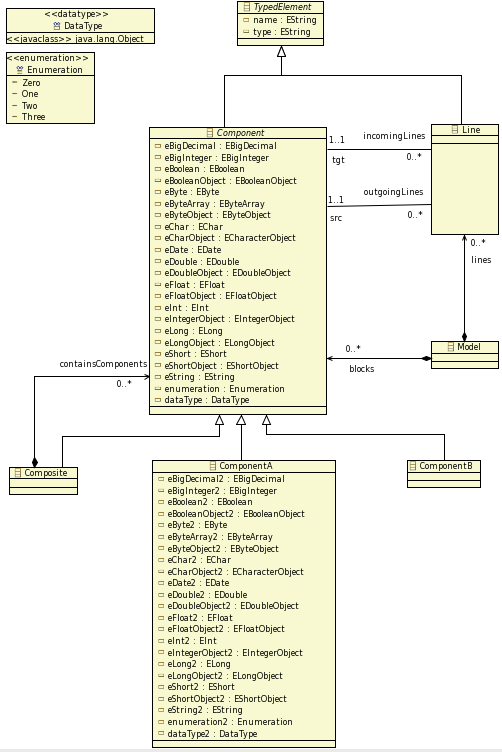
\includegraphics[scale=0.8]{img/testmetamodel.png}
	% testmetamodel.png: 502x752 pixel, 96dpi, 13.28x19.89 cm, bb=0 0 376 564
	\label{img_testmetamodel}
	\caption{Testmetamodell}
\end{figure}

\section{Erstellung von Testmetamodell-Instanzen}
Für die Erstellung von Testmetamodell-Instanzen exisitieren verschiedene Möglichkeiten, von denen hier zwei näher betrachtet werden sollen:
\begin{enumerate}
 \item Mittels des durch EMF bereit gestellten, generischen Ecore-Editors. Hat den Nachteil, dass es teilweise mühsam sein kann, die Graph-Struktur der Modelle zu erfassen. Das gilt sowohl für die Erstellung der Testdaten, als auch für die Nachvollziehbarkeit der einzelnen Testfälle.
 \item Instanzen werden in UML-Notation mittels eines UML-Tools spezifiziert und über einen Konverter nach EMF transformiert.
\end{enumerate}
Aus Gründen der Nachvollziehbarkeit und der leichteren Erstellung von Testmodellen werden wir die 2.te Variante anwenden. Als UML-Werkzeug ist der IBM Rational Software Modeler (RSM) in der Version 7.5 zu benutzen. Im Folgenden werden die einzelnen Schritte zur Erstellung von Testmodellen beschrieben.


\subsection{Modellerstellung in RSM}
Alle Testmodelle sind im RSM zu erstellen. Hierzu existieren zwei RSM-Projekte, TestmetamodelProfile und TestModels, welche im Verzeichnis \texttt{rsm/workspace} des Bundles \texttt{org.sidiff.common.testmodels} zu finden sind. Das Projekt TestmetamodelProfile definiert einige zur Identifikation von Komponenten benötigte Stereotypen (s. unten). Die eigentlichen Testmodelle werden im Projekt TestModels spezifiziert. 

\subsubsection{Pakethierarchie} 
Testmodelle werden in einer Pakethierarchie organisiert, welche folgenden Konventionen genügt (s. Abbildung \ref{img:package-hierarchie}):

\begin{itemize}
 \item Auf oberster Ebene befindet sich das Paket, welches die JUnit-Testfälle beinhaltet. Das Paket heißt wie das jeweilige OSGI-Bundle (z.B. org.sidiff.compare.comparefunctions.emf.test)
 \item Auf der nächsttieferen Ebene befindet sich das Paket, welche alle Testdaten für eine spezielle Compare-Funktion Test-Suite (z.B. CompareAttributeUsingLCSTest) beinhaltet.
 \item Auf der nächsten Hierarchie-Ebene befinden sich Pakete für alle Testfälle. Diese Pakete werden entsprechend dem Namensmuster $testcase_<NR.>$ benannt, wobei $<NR.>$ einer sequenziell hochgezählten Nummer entspricht.
 \item Für jeden Testfall werden schließlich die Eingabemodelle (in der Regel zwei) spezifiziert, welche sich in Unterpakten model-1 bzw. model-2 befinden. 
\end{itemize}

\begin{figure}
	\centering
 	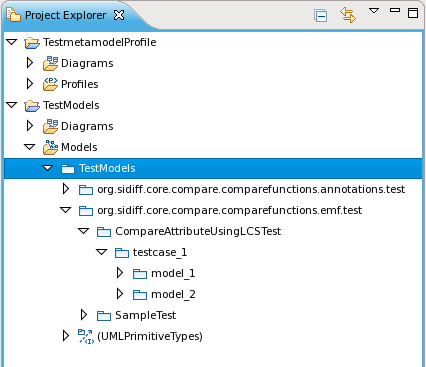
\includegraphics[scale=0.8]{img/package-hierarchie.png}
	\label{img:package-hierarchie}
	\caption{Exemplarische Paket-Hierarchie}
\end{figure}

\subsubsection{Spezifikation der eigentlichen Testmodelle}
Die eigentlichen Testmodelle werden in den oben beschriebenen Paketen model-1 bzw. model-2 spezifiziert. Zur grafischen Visualisierung ist ein Klassendiagramm zu verwenden. Abbildung \ref{img:sample-instance} zeigt ein Exemplarisches Testmodell in Klassendiagramm-Notation, Abbildung \ref{img:sample-instance-structure} die dazugehörige Modellstruktur, wie sie im RSM im Projekt-Explorer dargestellt wird. 

\begin{figure}
	\centering
 	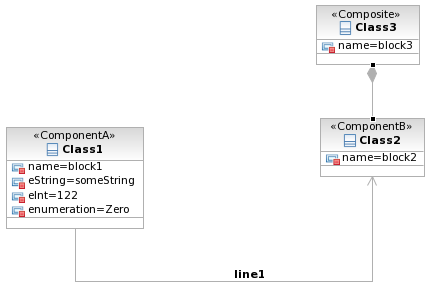
\includegraphics[scale=0.8]{img/sample-instance.png}
	\label{img:sample-instance}
	\caption{Exemplarisches Testmodell in UML-Klassendiagramm Notation}
\end{figure}

\begin{figure}
	\centering
 	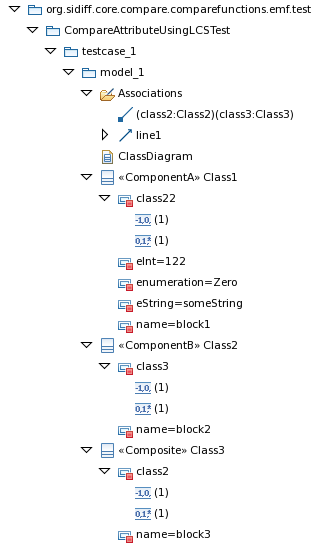
\includegraphics[scale=0.8]{img/sample-instance-structure.png}
	\label{img:sample-instance-structure}
	\caption{Exemplarische Modellstruktur}
\end{figure}

Die im Testmetamodell definierten Metaklassen werden durch folgende UML-Konstrukte umgesetzt:
\begin{itemize}
 \item ComponentA: Entspricht einer Klasse mit dem Stereotyp ComponentA (welcher in TestmetamodelProfile als Erweiterung der UML-Metaklasse Class definiert ist).
 \item ComponentB: Entspricht einer Klasse mit dem Stereotyp ComponentB (welcher in TestmetamodelProfile als Erweiterung der UML-Metaklasse Class definiert ist).
 \item Composite: Entspricht einer Klasse mit dem Stereotyp Composite (welcher in TestmetamodelProfile als Erweiterung der UML-Metaklasse Class definiert ist). Die Beziehung containsComponent ist durch eine Kompositionsbeziehung umzusetzen.
 \item Line: Lines werden durch gerichtete Assoziationen abgebildet. Rollennamen und Kardinalitäten brauchen nicht spezifiziert zu werden.
\end{itemize}

\subsubsection{Einschränkungen und Konventionen}
Folgende Einschränkungen und Konventionen sind zu beachten:
\begin{itemize}
 \item Attribute: Die Zuordnung von durch das Testmetamodell definierten Attributen und Attributwerten geschieht über die Benennung eines UML-Attributs nach folgendem Muster: $<attr-name>=<attr-value>$, wobei $<attr-name>$ dem Namen eines Attributs im Testmetamodell und $<attr-value>$ dem dazugehörigen Attributwert entspricht. Für einen Testfall nicht relevante Attribute müssen nicht spezifiziert zu werden. 
 \item Eindeutige Identifizierer: Modellelemente müssen eindeutig identifizierbar sein. Für alle Komponenten (ComponentA, ComponentB, Composite) ist daher das Attribut name unbedingt anzugeben. Auch Lines müssen identifizierbar sein. Als eindeutiger Identifizierer dient hier der Assoziationsname.
\end{itemize}

\subsection{Modellexport und Generierung von EMF-Modellen}
Um aus den im RSM erstellten UML-Modellen EMF-Modelle als die eigentlichen Testdaten der JUnit-Testfälle zu erhalten, sind diese zunächst im Eclipse UML2-Format zu exportieren und anschließend durch einen Konverter nach EMF zu transformieren. Beide Schritte werden im Folgenden beschrieben.

\subsubsection{Modellexport} Der Modellexport untergliedert sich in die folgenden Schritte:\\

\textbf{Schritt 1:} Rechtsklick auf das RSM-Projekt TestModels $>$ Export.\\

\textbf{Schritt 2:} Auswahl der Kategorie Other $>$ UML 2.1 Model (s. Abb. \ref{img:export-wizard-1}).\\
\begin{figure}
	\centering
 	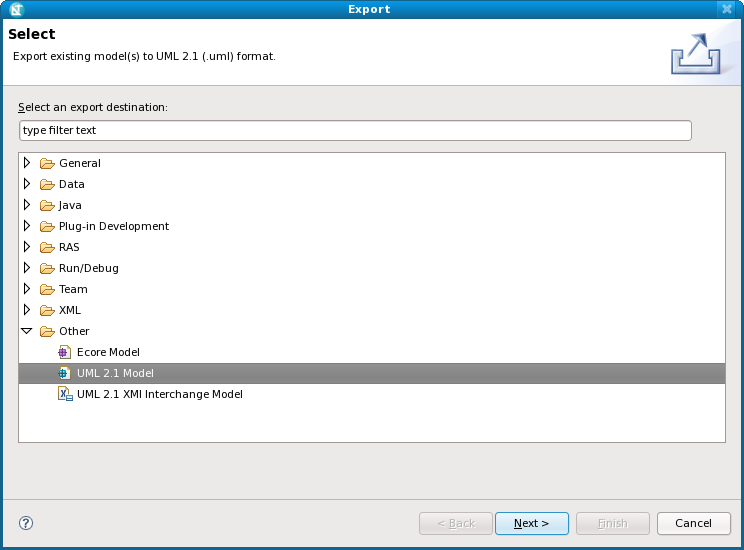
\includegraphics[scale=0.6]{img/export-wizard-1.png}
	\label{img:export-wizard-1}
	\caption{Export Wizard (1)}
\end{figure}

\textbf{Schritt 3:} Auswahl des zu exportierenden Modells und des Zielverzeichnisses, für welches das Verzeichnis \texttt{rsm/export} im Bundle \texttt{org.sidiff.common.testmodels} zu wählen ist. \textbf{Wichtig:} Unbedingt die Option Export applied profiles aktivieren! (s. Abb. \ref{img:export-wizard-2}).\\
\begin{figure}
	\centering
 	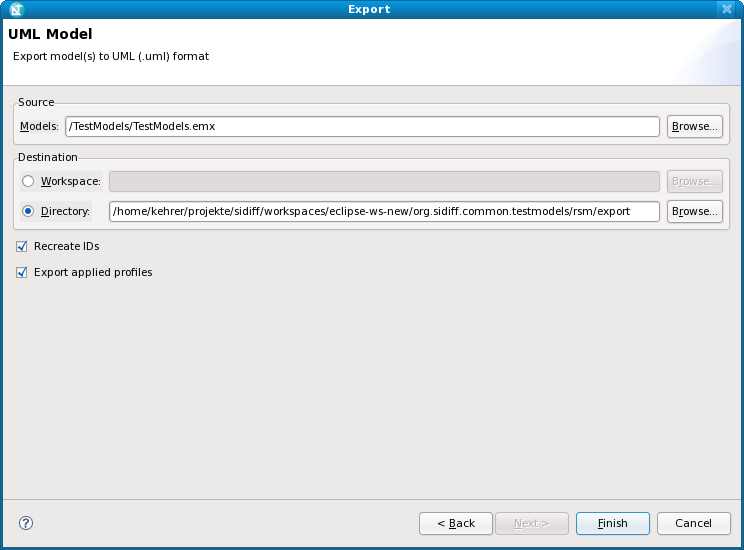
\includegraphics[scale=0.6]{img/export-wizard-2.png}
	\label{img:export-wizard-2}
	\caption{Export Wizard (2)}
\end{figure}


\subsubsection{Generierung von EMF-Modellen}
Um EMF-Modelle zu generieren, muss eine OSGI-Konsole mit dem Bundle org.sidiff.common.testmodels gestartet werden. Dieses nimmt ein Kommando generate $<WORKSPACE-URI>$ entgegen, wobei $<WORKSPACE-URI>$ den Betriebssystem-absoluten Pfad zu dem für die SiDiff-Entwicklung genutzten Eclipse-Workspace darstellt. Um die ständige Eingabe dieses Parameters zu vermeiden, kann in der Klasse \texttt{TestdataGeneratorCommandProvider} im Bundle und gleichnamigen Paket \texttt{org.sidiff.common.testmodels} ein neues Kommando spezifiziert werden, welches die private Methode generate(String workspaceUri) aufruft. Beispiel: 
\begin{lstlisting}
public void _generateTK(CommandInterpreter commandInterpreter) throws Exception {
	generate("/home/kehrer/projekte/sidiff/workspaces/eclipse-ws-new");
}
\end{lstlisting}

Die generierten EMF-Modelle werden in den jeweiligen Bundles zum Testen der Compare-Funktionen abgelegt.
	%
% Aufbau und Validierung einer Konfigurationsdatei
% ===========================================================================
%

\chapter{Einrichten und Ausführen der Unit-Tests}
\label{strct:intro}

Checkout der relevanten Bundles. Für die Unit-Tests der EMF Funktionen sind 
dies beispielsweise
	
\begin{itemize}
	\item org.sidiff.commons
	\item org.sidiff.common.emf
	\item org.sidiff.common.junit
	\item org.sidiff.common.services
	\item org.sidiff.common.testmetamodel
	\item org.sidiff.core.compare.comparefunctions
	\item org.sidiff.core.compare.comparefunctions.emf
	\item org.sidiff.core.compare.comparefunctions.emf.test
\end{itemize}

Starten des Activators in org.sidiff.common.junit als neue OSGi Framework
Run-Konfiguration.\\

Reiter Bundles: Auswahl der benötigten bundles (i.d.R. Workspace + required
Bundles)\\
		
Reiter Arguments: Wichtig! Das Working Directory auf den lokalen Workspace
setzen. Dies ist nötig damit die zu testenden Models später über relative
Pfade gefunden werden können!\\

Einstellungen übernehmen und starten. In der OSGi Konsole sampleTest zum 
Starten des Beispiels tippen und Return drücken...
	%
% Dokumentation der Vergleichsfunktionen
% ===========================================================================
%

\chapter{Dokumentation der Vergleichsfunktionen}
\label{strct:spec}
An dieser Stelle seien nun die einzelnen vom SiDiff-Kern bereitgestellten Vergleichsfunktionen dokumentiert. Die Vergleichsfunktionen werden dabei anhand ihrer Semantiken gruppiert oder, sofern diese sich keiner allgemeinen Gruppe zuordnen lassen, dem folgenden \structgetfullref{strct:spec:misc} zugeschrieben.

\begin{tabular}[ht]{|l|l|}
\hline
new CF & reviewed \\
\hline
\hline
CompareAttributeUsingEquals & \\
\hline
CompareAttributeUsingGauss & \\
\hline
CompareAttributeUsingIndexOf & \\
\hline
CompareAttributeUsingLcs & \\
\hline

\end{tabular}

\begin{tabular}[ht]{|l|l|c|c|}
\hline
old CF & new CF & TestData & tested \\
\hline
\hline
\textbf{org.sidiff.core.compare.comparefunctions.} & \multirow{2}{*}{ } & \multirow{2}{*}{ } & \multirow{2}{*}{ }\\
\textbf{emf} & & & \\
\hline
\textit{Abstract} & & & \\
\hline
AbstractAllReferences & & & \\
\hline
AbstractAllReferencesHasThreshold & & & \\
\hline
AbstractAttribute & & & \\
\hline
AbstractChildren & & & \\
\hline
AbstractChildrenHasThreshold & & & \\
\hline
AbstractNumericAttribute & & & \\
\hline
AbstractParents & & & \\
\hline
AbstractReferences & & & \\
\hline
AbstractReferecnesHasThreshold & & & \\
\hline
AbstractRemoteNodes & & & \\
\hline
AbstractRemoteNodesHasThreshold & & & \\
\hline
AbstractStringAttribute & & & \\
\hline
\textit{Implementations} & & & \\
\hline
AllReferenceEqualViewingTypes & & & \\
\hline
BooleanAttribute & CompareAttributeUsingEquals & x & x\\	
\hline
ChildrenEqualViewingTypes & & &\\	
\hline
EnumerationAttribute & & &\\	
\hline
EqualID & & &\\	
\hline
ExplicitMatch & & &\\	
\hline
MaximumSimilarity & & &\\	
\hline
NoSimilarity & & &\\	
\hline
NumericAttributeEqualUsingDouble & CompareAttributeUsingEquals & x & x\\	
\hline
NumericAttributeEqualUsingFloat & CompareAttributeUsingEquals & x & x\\	
\hline
NumericAttributeEqualUsingInteger & CompareAttributeUsingEquals & x & x\\	
\hline
NumericAttributeEqualUsingLong & CompareAttributeUsingEquals & x & x\\	
\hline
NumericAttributeSimilarUsingGauss & CompareAttributeUsingGauss & x & x\\	
\hline
ReferenceExists & & &\\	
\hline
ReferencesEqualViewingTypes & & &\\	
\hline
RemoteNodesEqualViewingTypes & & &\\	
\hline
StringAttributeUsingBoyer & & &\\	
\hline
StringAttributeUsingEquals & CompareAttributeUsingEquals & x & x\\	
\hline
StringAttributeUsingIndexOf & CompareAttributeUsingIndexOf & x & x\\	
\hline
StringAttributeUsingLcs & CompareAttributeUsingLcs & x & x\\	
\hline

\end{tabular}

\begin{tabular}[ht]{|l|l|c|c|}
\hline
old CF & new CF & TestData & tested \\
\hline
\hline
\textbf{org.sidiff.core.compare.comparefunctions.} & \multirow{2}{*}{ } & \multirow{2}{*}{ } & \multirow{2}{*}{ }\\
\textbf{annotations} & & & \\
\hline
\textit{Abstract} & & & \\
\hline
AbstractNumericAnnotations & & & \\
\hline
AbstractStringAnnotations & & & \\
\hline
\textit{Implementations} & & & \\
\hline
AllReferencesEqualViewingAnnotation & & & \\
\hline
NumericAnnotationEqualUsingDouble & & & \\
\hline
NumericAnnotationEqualUsingFloat & & & \\
\hline
NumericAnnotationEqualUsingInteger & & & \\
\hline
NumericAnnotationEqualUsingLong & & & \\
\hline
NumericAnnotationSimilarUsingGauss & & & \\
\hline
ReferencesEqualViewingAnnotation & & & \\
\hline
RemoteNodesEqualViewingAnnotation & & & \\
\hline
StringAnnotationsUsingBoyer & & & \\
\hline
StringAnnotationUsingEquals & & & \\
\hline
StringAnnotationsUsingIndexOf & & & \\
\hline
StringAnnotationUsingLcs & & & \\
\hline

\end{tabular}

\begin{tabular}[ht]{|l|l|c|c|}
\hline
old CF & new CF & TestData & tested \\
\hline
\hline
\textbf{org.sidiff.core.compare.comparefunctions.} & \multirow{2}{*}{ } & \multirow{2}{*}{ } & \multirow{2}{*}{ }\\
\textbf{similarities} & & & \\
\hline
\textit{Implementations} & & & \\
\hline
AllReferencesSimilar & & & \\
\hline
ChildrenSimilar & & & \\
\hline
ParentsSimilar & & & \\
\hline
RefencesSimilar & & & \\
\hline
RemoteNodesSimilar & & & \\
\hline

\end{tabular}

\begin{tabular}[ht]{|l|l|c|c|}
\hline
old CF & new CF & TestData & tested \\
\hline
\hline
\textbf{org.sidiff.core.compare.comparefunctions.} & \multirow{2}{*}{ } & \multirow{2}{*}{ } & \multirow{2}{*}{ }\\
\textbf{correspondences} & & & \\
\hline
\textit{Implementations} & & & \\
\hline
AllReferencesEqualViewingMatches & & & \\
\hline
AllReferencesMatched & & & \\
\hline
ChildrenEqualViewingMatches & & & \\
\hline
ChildrenMatched & & & \\
\hline
ParentsMatched & & & \\
\hline
ReferencesEqualVewingMatches & & & \\
\hline
ReferencesMatched & & & \\
\hline
RemoteNodesEqualViewingMatches & & & \\
\hline
RemoteNodesMatched & & & \\
\hline

\end{tabular}

\begin{tabular}[ht]{|l|l|c|c|}
\hline
old CF & new CF & TestData & tested \\
\hline
\hline
\textbf{org.sidiff.core.compare.comparefunctions.} & \multirow{2}{*}{ } & \multirow{2}{*}{ } & \multirow{2}{*}{ }\\
\textbf{correspondencesorsimilarities} & & & \\
\hline
\textit{Implementations} & & & \\
\hline
AllReferencesMatchedOrSimilar & & & \\
\hline
ChildrenMatchedOrSimilar & & & \\
\hline
ParentsMatchedOrSimilar & & & \\
\hline
ReferencesMatchedOrSimilar & & & \\
\hline
RemoteNodesMatchedOrSimilar & & & \\
\hline
\end{tabular}


%
% Vergleichsfunktionen: Verschiedenartig
% ===========================================================================
%

\section{Verschiedenartige Vergleichsfunktionen}
\label{strct:spec:misc}
In diesem Abschnitt werden verschiedene Vergleichsfunktionen angeführt, die sich keiner größeren allgemeinen Gruppe zuordnen lassen.


%
% --> EqualID
%
\subsection{\texttt{EqualID}}
\subsubsection*{Vorbedingungen}
Für die Eingabeknoten müssen IDs existieren.
\subsubsection*{Semantik}
Die Eingabeknoten werden anhand der ID-Attribute miteinander verglichen.
\subsubsection*{Rückgabewert}
Für übereinstimmende IDs wird $1$ und für unterschiedliche $0$ zurückgegeben.
\subsubsection*{Parameter}
Keine


%
% --> ExplicitMatch
%
\subsection{\texttt{ExplicitMatch}}
\subsubsection*{Vorbedingungen}
Keine
\subsubsection*{Semantik}
Es wird \emph{kein} expliziter Vergleich durchgeführt. Diese Funktion liefert unabhängig von den übergebenen Eingabeknoten immer $1$.
\subsubsection*{Rückgabewert}
Es wird \emph{immer} $1$ als Similarity zurückgegeben.
\subsubsection*{Parameter}
Keine
\subsubsection*{Abgefangene Fehler}
Sind für den SiDiff-Kern Debug-Ausgaben aktiviert, so kann im Ausnahmefall eine\mylinebreak\textclass{SiDiffRuntimeException} ausgelöst werden.


\newpage
%
% --> MaximumSimilarity
%
\subsection{\texttt{MaximumSimilarity}}
\subsubsection*{Vorbedingungen}
Keine
\subsubsection*{Semantik}
Es wird \emph{kein} expliziter Vergleich durchgeführt. Diese Funktion liefert unabhängig von den übergebenen Eingabeknoten immer $1$.
\subsubsection*{Rückgabewert}
Es wird \emph{immer} $1$ als Similarity zurückgegeben.
\subsubsection*{Parameter}
Keine


%
% --> CINoSimilarity
%
\subsection{\texttt{NoSimilarity}}
\subsubsection*{Vorbedingungen}
Keine
\subsubsection*{Semantik}
Es wird \emph{kein} expliziter Vergleich durchgeführt. Diese Funktion liefert unabhängig von den übergebenen Eingabeknoten immer $0$.\\
Es handelt sich um eine Vergleichsfunktion, mit der sich Knotentypen vom Vergleich ausschließen lassen.
\subsubsection*{Rückgabewert}
Es wird \emph{immer} $0$ als Similarity zurückgegeben.
\subsubsection*{Parameter}
Keine

\newpage
%
% Vergleichsfunktionen: String-Attribut
% ===========================================================================
%

\section{\texttt{StringAttribute}...}
\label{strct:spec:stringattr}
Dieser Abschnitt behandelt Vergleichsfunktionen des Typs \texttt{StringAttribute}, mit Hilfe derer sich die Zeichenketten von Attributen der aktuellen Eingabeknoten vergleichen lassen. Allgemein lassen sich bereits folgende Angaben zu dieser Gruppe von Vergleichsfunktionen machen.

\subsubsection*{Allgemeine Vorbedingungen}
Für den Fall, dass explizit ein einzelnes Attribut zum Vergleich angegeben wird, muss dieses existieren. Ist dies nicht der Fall erfolgt die Auslösung einer Ausnahme des Typs\mylinebreak\texttt{AttributeNotExistsException} oder \texttt{AnnotationNotExistsException} im Fall eines zu vergleichenden virtuellen Attributs. Eine \texttt{AttributeNotExistsException} wird auch ausgelöst, wenn der im Parameter spezifizierte reguläre Ausdruck keine zu vergleichenden Attributnamen liefert.\\
In jedem der drei oben aufgeführten Fälle terminiert der SiDiff-Kern unverzüglich die Ausführung des Vergleichauftrags.

\subsubsection*{Allgemeine Semantik}
Die Eingabeknoten werden über ein oder mehrere durch den Parameter definierte Attribute miteinander verglichen. Der Vergleich der Attributwerte erfolgt nach der in der jeweiligen Vergleichsfunktion spezifizierten Methode.\\
Anzumerken ist, dass sich mittels dieser Klasse von Vergleichsfunktionen auch explizit \emph{virtuelle} Attribute miteinander vergleichen lassen. Mehr dazu unter \textcrosslink{Allgemeiner Parameter}.

Es bestehen zwei grundsätzliche Optionen:
\begin{enumerate}
	\item Es wird lediglich ein Attribut zum Vergleich angegeben.
	\item Mittels eines regulären Ausdrucks werden mehrere Attribute spezifiziert, die für den Vergleich herangezogen oder von diesem ausgeschlossen werden sollen.
\end{enumerate}

Siehe dazu auch \textcrosslink{Allgemeine Parameter}.

\subsubsection*{Allgemeiner Rückgabewert}
\begin{enumerate}
	\item Es werden \emph{keine} regulären Ausdrücke verwendet – also \emph{ein} Attribut soll verglichen werden:
		\begin{itemize}
			\item Wenn bei beiden Eingabeknoten das zu vergleichende Attribut nicht vorhanden ist, so wird $1$ zurückgegeben.
			\item Ist das zu vergleichende Attribut bei lediglich einem Eingabeknoten nicht vorhanden, wird $0$ zurückgegeben.
			\item Sind beide Attributwerte vorhanden, so wird unter Anwendung der entsprechenden Vergleichsmethode die Ähnlichkeit bestimmt und als Similarity zurückgegeben.
		\end{itemize}
	\item Reguläre Ausdrücke werden verwendet (i.d.R. sollen \emph{mehrere} Attribute verglichen werden):
		\begin{itemize}
			\item Wenn keines der zu vergleichenden Attribute existiert, wird $1$ als Ähnlichkeit zurückgegeben.
			\item Sofern zu vergleichende Attribute nach Anwendung des regulären Ausdrucks vorliegen, werden die Attribute einzeln miteinander verglichen und die einzelnen Ähnlichkeiten aufaddiert.\\
			Zurückgegeben wird der Quotient aus den kumulierten Einzel-Ähnlichkeiten und der Anzahl der durch den regulären Ausdruck gefundenen Anzahl an zu vergleichenden Attributen.\\
			\textnoticesec{Bemerkung:} Der Vergleich der \emph{einzelnen} Attribute erfolgt nach den gleichen Gesichtspunkten, wie in der Vergleichsoption \emph{ohne} Verwendung regulärer Ausdrücke (s.o.).
		\end{itemize}
\end{enumerate}

\subsubsection*{Allgemeine Parameter}
Als Parameter wird der Namen des zu vergleichenden Attributs übergeben.\\
Ebenso ist es möglich mittels eines \emph{regulären Ausdrucks} mehrere Attribute explizit zum Vergleich anzugeben oder alle Attribute bis auf eine durch einen regulären Ausdruck definierte Ausschlussliste zum Vergleich zu markieren. Im ersteren Fall wird dem regulären Ausdruck ein "`$+$"' vorangestellt; im Falle einer Ausschlussliste ein "`$-$"'.

Neben den beiden oben genannten Möglichkeiten, besteht auch die Möglichkeit explizit ein \emph{virtuelles} Attribut zum Vergleich zu markieren. Dazu wird dem Attributnamen lediglich ein $\$$ vorangestellt. Für den Vergleich von virtuellen Attributen werden allerdings \emph{keine} regulären Ausdrücke unterstützt, sodass immer nur ein spezielles Attribut vergleichbar ist.

\vskip15pt
%
% --> StringAttributeUsingBoyerCI
%
\subsection{\texttt{StringAttributeUsingBoyerCI}}
Diese Vergleichsfunktion führt Vergleiche anhand den unter \structgetfullref{strct:spec:stringattr} aufgeführten allgemeinen Bedingungen durch.

\subsubsection*{Spezielle Semantik und Rückgabewert}
Als spezielle Vergleichsmethode wird in diesem Fall der \emph{case-insensitive} Vergleich nach \emph{Boyer} verwendet.


%
% --> StringAttributeUsingBoyerCS
%
\subsection{\texttt{StringAttributeUsingBoyerCS}}
Diese Vergleichsfunktion führt Vergleiche anhand den unter \structgetfullref{strct:spec:stringattr} aufgeführten allgemeinen Bedingungen durch.

\subsubsection*{Spezielle Semantik und Rückgabewert}
Als spezielle Vergleichsmethode wird in diesem Fall der \emph{case-sensitive} Vergleich nach \emph{Boyer} verwendet.


%
% --> StringAttributeUsingEqualsCI
%
\subsection{\texttt{StringAttributeUsingEqualsCI}}
Diese Vergleichsfunktion führt Vergleiche anhand den unter \structgetfullref{strct:spec:stringattr} aufgeführten allgemeinen Bedingungen durch.

\subsubsection*{Spezielle Semantik und Rückgabewert}
Als spezielle Vergleichsmethode wird in diesem Fall der \emph{case-insensitive Equals}-Vergleich verwendet. Dies bedeutet, dass die Zeichenketten auf Gleichheit -- allerdings nicht im Sinne der Groß- und Kleinschreibung -- verglichen werden.


%
% --> StringAttributeUsingEqualsCS
%
\subsection{\texttt{StringAttributeUsingEqualsCS}}
Diese Vergleichsfunktion führt Vergleiche anhand den unter \structgetfullref{strct:spec:stringattr} aufgeführten allgemeinen Bedingungen durch.

\subsubsection*{Spezielle Semantik und Rückgabewert}
Als spezielle Vergleichsmethode wird in diesem Fall der \emph{case-insensitive Equals}-Vergleich verwendet. Dies bedeutet, dass die Zeichenketten auf exakte Gleichheit -- auch im Sinne der Groß- und Kleinschreibung -- verglichen werden.


\newpage
%
% --> StringAttributeUsingIndexOfCI
%
\subsection{\texttt{StringAttributeUsingIndexOfCI}}
Diese Vergleichsfunktion führt Vergleiche anhand den unter \structgetfullref{strct:spec:stringattr} aufgeführten allgemeinen Bedingungen durch.

\subsubsection*{Spezielle Semantik und Rückgabewert}
Als spezielle Vergleichsmethode wird in diesem Fall der \emph{case-insensitive IndexOf}-Vergleich verwendet. Dies bedeutet, dass überprüft wird, ob die Zeichenketten sich gegenseitig beinhalten. Beinhaltet bspw. Zeichenkette A des einen Attributs die Zeichenkette B des Attributs im gegenüberliegenden Knoten, so wird als Ähnlichkeit der Quotient aus der kürzeren Zeichenkette B und der längeren Zeichenkette A zurückgegeben. Die Groß- und Kleinschreibung spielen bei dieser Variante allerdings \emph{keine} Rolle.


%
% --> StringAttributeUsingIndexOfCS
%
\subsection{\texttt{StringAttributeUsingIndexOfCS}}
Diese Vergleichsfunktion führt Vergleiche anhand den unter \structgetfullref{strct:spec:stringattr} aufgeführten allgemeinen Bedingungen durch.

\subsubsection*{Spezielle Semantik und Rückgabewert}
Als spezielle Vergleichsmethode wird in diesem Fall der \emph{case-sensitive IndexOf}-Vergleich verwendet. Dies bedeutet, dass überprüft wird, ob die Zeichenketten sich gegenseitig beinhalten. Beinhaltet bspw. Zeichenkette A des einen Attributs die Zeichenkette B des Attributs im gegenüberliegenden Knoten, so wird als Ähnlichkeit der Quotient aus der kürzeren Zeichenkette B und der längeren Zeichenkette A zurückgegeben. Zusätzlich wird bei dieser Variante die Groß- und Kleinschreibung beachtet.

%
% --> StringAttributeUsingLcsCI
%
\subsection{\texttt{StringAttributeUsingLcsCI}}
Diese Vergleichsfunktion führt Vergleiche anhand den unter \structgetfullref{strct:spec:stringattr} aufgeführten allgemeinen Bedingungen durch.

\subsubsection*{Spezielle Semantik und Rückgabewert}
Als spezielle Vergleichsmethode wird in diesem Fall der \emph{case-insensitive LCS}-Vergleich verwendet. Dies bedeutet, dass innerhalb beider Zeichenketten die längste, gemeinsamste Teilsequenz gesucht wird und letztlich der Quotient der Länge dieser und der Länge des längeren Attributwerts als Ähnlichkeit zurückgegeben wird. Bei dieser Variante ist die Groß- und Kleinschreibung allerdings \emph{nicht} von Belang.

%
% --> StringAttributeUsingLcsCS
%
\subsection{\texttt{StringAttributeUsingLcsCS}}
Diese Vergleichsfunktion führt Vergleiche anhand den unter \structgetfullref{strct:spec:stringattr} aufgeführten allgemeinen Bedingungen durch.

\subsubsection*{Spezielle Semantik und Rückgabewert}
Als spezielle Vergleichsmethode wird in diesem Fall der \emph{case-insensitive LCS}-Vergleich verwendet. Dies bedeutet, dass innerhalb beider Zeichenketten die längste, gemeinsamste Teilsequenz gesucht wird und letztlich der Quotient der Länge dieser und der Länge des längeren Attributwerts als Ähnlichkeit zurückgegeben wird. Die Groß- und Kleinschreibung ist bei dieser Variante von Belang!
\newpage
%
% Vergleichsfunktionen: Numerisches Attribut
% ===========================================================================
%

\section{\texttt{NumericAttribute}...}
\label{strct:spec:numattr}
Dieser Abschnitt behandelt Vergleichsfunktionen des Typs \texttt{NumericAttribute}, mit Hilfe derer sich numerische Attributwerte der aktuellen Eingabeknoten vergleichen lassen. Allgemein lassen sich bereits folgende Angaben zu dieser Gruppe von Vergleichsfunktionen machen.

\subsubsection*{Allgemeine Vorbedingungen}
Für den Fall, dass explizit ein einzelnes Attribut zum Vergleich angegeben wird, muss dieses existieren. Ist dies nicht der Fall erfolgt die Auslösung einer Ausnahme des Typs\mylinebreak\texttt{AttributeNotExistsException} oder \texttt{AnnotationNotExistsException} im Fall eines zu vergleichenden virtuellen Attributs. Eine \texttt{AttributeNotExistsException} wird auch ausgelöst, wenn der im Parameter spezifizierte reguläre Ausdruck keine zu vergleichenden Attributnamen liefert.\\
In \emph{jedem} Fall muss das auszuwertende Attribut einen numerischen Wert beinhalten. Ist diese Voraussetzung nicht gegeben, löst die Vergleichsfunktion eine Ausnahme vom Typ\mylinebreak\texttt{InvalidAttributeValue} aus und der SiDiff-Kern terminiert -- wie in den anderen o.g. Szenarien -- unverzüglich die Ausführung des Vergleichauftrags.

\subsubsection*{Allgemeine Semantik}
Diese Gruppe der Vergleichsfunktionen führt den Vergleich von Eingabeknoten aufgrund eines \emph{numerischen} Attributs durch. Dabei wird im Parameter der Name des zu vergleichenden, numerischen Attributs angegeben. Die spezielle Vergleichsmethode ist in den implementierenden Vergleichsfunktionen, die weiter unten in diesem Abschnitt gefunden werden können, spezifiziert und genauer erläutert.

\subsubsection*{Allgemeiner Rückgabewert}
\begin{itemize}
	\item Sofern für beide Eingabeknoten das im Parameter spezifizierte Attribut existiert, wird anhand der entsprechenden Vergleichsmethode die Ähnlichkeit der beiden numerischen Attributwerte bestimmt und zurückgegeben.
	\item Existiert für einen oder gar beide Eingabeknoten das angegebene Attribut nicht, beträgt die Ähnlichkeit $0$.
	\item Die Ähnlichkeit beträgt ebenfalls $0$, sofern einer der beiden Attributwerte nicht numerisch ist und somit kein Vergleich durchgeführt werden kann.
\end{itemize}

\subsubsection*{Allgemeine Parameter}
Die Parameter der implementierenden Vergleichsfunktionen unterscheiden sich teilweise. In jedem Fall muss jedoch der Name des zu vergleichenden Attributs übergeben werden.\\
Mehr zum genaueren Parameterformat im Abschnitt \textcrosslink{Spezielle Parameter} der jeweiligen Vergleichsfunktion.


\newpage
%
% --> NumericAttributeSimilarUsingDouble
%
\subsection{\texttt{NumericAttributeSimilarUsingGauss}}
Diese Vergleichsfunktion führt Vergleiche anhand den unter \structgetfullref{strct:spec:numattr} aufgeführten allgemeinen Bedingungen durch.

\subsubsection*{Spezielle Parameter}
Diese Vergleichsfunktion benötigt zwei Parameter, die durch "`\texttt{;}"' voneinander abgetrennt werden. Folgend beide Unter-Parameter in der anzugebenden Reihenfolge:
\begin{enumerate}
	\item Der Name des zu vergleichenden, numerischen Attributs.
	\item Ein Skalierungsfaktor, der in die Ähnlichkeitsberechnung eingeht.\\
		Mehr dazu unter \textcrosslink{Spezielle Semantik und Rückgabewert}.
\end{enumerate}
Ein gültiger Parameter wäre also:  \texttt{myattribute;0.75}

Sofern ein ungültiges Parameterformat übergeben wird oder der Skalierungsfaktor nicht parsbar ist, erfolgt die Auslösung einer Ausnahme des Typs \texttt{InvalidParameterSyntaxException}.

\subsubsection*{Spezielle Semantik und Rückgabewert}
Diese Vergleichsfunktion vergleicht Ganz- bzw. 64-Bit Fließkomma-Zahlen vom Typ \texttt{Double} anhand der \emph{Gaußschen Normalverteilung} auf Ähnlichkeit. Dazu wird im Parameter dieser Vergleichsfunktion ebenfalls ein Skalierungsfaktor angegeben, um die Form der Glockenkurve individuell beeinflussen zu können.

\dotuline{Im Detail:}
\begin{itemize}
	\item Zwischen beiden Attributwerten wird die Differenz gebildet und diese quadriert. Danach wird der Quotient aus der quadrierten Differenz und dem Skalierungsfaktor gebildet und das negierte Zwischenergebnis letztlich auf die Eulersche Exponentialfunktion angewandt.
	\item In mathematischer Form wie folgt:  $exp\left(-\frac{(value1 - value2)^2}{scale}\right)$
\end{itemize}


%
% --> NumericAttributeEqualUsingInteger
%
\subsection{\texttt{NumericAttributeEqualUsingInteger}}
Diese Vergleichsfunktion führt Vergleiche anhand den unter \structgetfullref{strct:spec:numattr} aufgeführten allgemeinen Bedingungen durch.

\subsubsection*{Spezielle Parameter}
Diese Vergleichsfunktion benötigt als Parameter lediglich den Namen des zu vergleichenden numerischen Attributs.

\subsubsection*{Spezielle Semantik und Rückgabewert}
Diese Vergleichsfunktion vergleicht \textbf{\texttt{Integer}}-Werte (also 32-Bit große Ganzzahl-Werte) auf Identität.
\begin{itemize}
	\item Sind beide Attributwerte gleich, so beträgt die Ähnlichkeit $1$.
	\item Bei verschiedenen Attributwerten wird $0$ zurückgegeben.
\end{itemize}


\newpage
%
% --> NumericAttributeEqualUsingFloat
%
\subsection{\texttt{NumericAttributeEqualUsingFloat}}
Diese Vergleichsfunktion führt Vergleiche anhand den unter \structgetfullref{strct:spec:numattr} aufgeführten allgemeinen Bedingungen durch.

\subsubsection*{Spezielle Parameter}
Diese Vergleichsfunktion benötigt als Parameter lediglich den Namen des zu vergleichenden numerischen Attributs.

\subsubsection*{Spezielle Semantik und Rückgabewert}
Diese Vergleichsfunktion vergleicht \textbf{\texttt{Float}}-Werte (also 32-Bit große Fließkomma-Zahlen) auf Identität.
\begin{itemize}
	\item Sind beide Attributwerte gleich, so beträgt die Ähnlichkeit $1$.
	\item Bei verschiedenen Attributwerten wird $0$ zurückgegeben.
\end{itemize}


%
% --> NumericAttributeEqualUsingDouble
%
\subsection{\texttt{NumericAttributeEqualUsingDouble}}
Diese Vergleichsfunktion führt Vergleiche anhand den unter \structgetfullref{strct:spec:numattr} aufgeführten allgemeinen Bedingungen durch.

\subsubsection*{Spezielle Parameter}
Diese Vergleichsfunktion benötigt als Parameter lediglich den Namen des zu vergleichenden numerischen Attributs.

\subsubsection*{Spezielle Semantik und Rückgabewert}
Diese Vergleichsfunktion vergleicht \textbf{\texttt{Double}}-Werte (also 64-Bit große Fließkomma-Zahlen) auf Identität.
\begin{itemize}
	\item Sind beide Attributwerte gleich, so beträgt die Ähnlichkeit $1$.
	\item Bei verschiedenen Attributwerten wird $0$ zurückgegeben.
\end{itemize}
\newpage
%
% Vergleichsfunktionen: Parents
% ===========================================================================
%

\section{\texttt{Parents}...}
\label{strct:spec:parents}
Dieser Abschnitt behandelt Vergleichsfunktionen des Typs \texttt{Parents}, mit denen sich die Eingabeknoten anhand ihrer Elternknoten vergleichen lassen.

\subsubsection*{Allgemeine Vorbedingungen}
Mindestens einer der beiden Eingabeknoten sollte einen Elternknoten besitzen.\\
Ist dieses nicht der Fall -- z.B. wenn die Eingabeknoten Wurzelelemente darstellen --, wird eine Ausnahme des Typs \texttt{NothingToCompareException} ausgelöst.

\subsubsection*{Allgemeine Semantik}
Die Eingabeknoten werden anhand ihrer Elternknoten miteinander verglichen. Die genaue Art der Ähnlichkeitsbestimmung ist dabei in den implementierenden Vergleichsfunktionen, die weiter unten im Abschnitt eingesehen werden können, festgelegt.

\subsubsection*{Allgemeiner Rückgabewert}
\begin{itemize}
	\item Besitzt genau \emph{einer der beiden} Eingabeknoten keinen Elternknoten, so wird $0$ als Similarity zurückgegeben.
	\item Besitzen \emph{beide} Eingabeknoten keinen Elternknoten, so wird eine Ausnahme des Typs\mylinebreak\texttt{NothingToCompareException} ausgelöst.
	\item Für den übrigen Fall -- also wenn für beide Eingabeknoten Elternknoten existieren -- erfolgt die Ähnlichkeitsbestimmung anhand der Semantik der speziellen Vergleichsfunktion (s.u.).
\end{itemize}

\subsubsection*{Allgemeine Parameter}
Keine der Vergleichsfunktionen dieses Typs benötigen einen Parameter.



%
% --> ParentsMatchedOrSimilar
%
\subsection{\texttt{ParentsMatchedOrSimilar}}
Diese Vergleichsfunktion führt Vergleiche anhand den unter \structgetfullref{strct:spec:parents} aufgeführten allgemeinen Bedingungen durch.

\subsubsection*{Spezielle Semantik und Rückgabewert}
Die Eingabeknoten werden anhand der direkten Übereinstimmung bzw. der Ähnlichkeit der Elternknoten miteinander verglichen. Zunächst wird also geprüft, ob die Elternknoten bereits übereinstimmen -- ist dies nicht der Fall, so erfolgt der Vergleich aufgrund der Ähnlichkeiten der Elternknoten untereinander.

Als Ähnlichkeit der Eingabeknoten wird also letztlich bei Übereinstimmung der Elternknoten $1$, andernfalls die bekannte Ähnlichkeit der beiden Elternknoten zurückgegeben.

\textnoticesec{Bemerkung:} Diese Vergleichsfunktion ist nicht reflexiv.


%
% --> ParentsMatched
%
\subsection{\texttt{ParentsMatched}}
Diese Vergleichsfunktion führt Vergleiche anhand den unter \structgetfullref{strct:spec:parents} aufgeführten allgemeinen Bedingungen durch.

\subsubsection*{Spezielle Semantik und Rückgabewert}
Die Eingabeknoten werden anhand ihrer Elternknoten miteinander verglichen. Dabei werden allein \emph{Übereinstimmungen} berücksichtigt. Es erfolgt also \emph{kein} Vergleich aufgrund von Ähnlichkeiten.

Bei Übereinstimmung der Elternknoten wird $1$, andernfalls $0$ als Ähnlichkeit zurückgegeben.


\newpage
%
% --> ParentsSimilar
%
\subsection{\texttt{ParentsSimilar}}
Diese Vergleichsfunktion führt Vergleiche anhand den unter \structgetfullref{strct:spec:parents} aufgeführten allgemeinen Bedingungen durch.

\subsubsection*{Spezielle Semantik und Rückgabewert}
Die Eingabeknoten werden anhand ihrer Elternknoten miteinander verglichen. Dabei werden allein die bekannten \emph{Ähnlichkeitswerte} der Eltern berücksichtigt. Es erfolgt also \emph{kein} Vergleich aufgrund von Übereinstimmungen.

Als Ähnlichkeit der beiden Eingabeknoten wird somit die Ähnlichkeit der beiden Elternknoten zurückgegeben.

\textnoticesec{Bemerkung:} Diese Vergleichsfunktion ist nicht reflexiv.


%
% --> ParentsEqualHash
%
\subsection{\texttt{ParentsEqualHash}}
Diese Vergleichsfunktion führt Vergleiche anhand den unter \structgetfullref{strct:spec:parents} aufgeführten allgemeinen Bedingungen durch.

\subsubsection*{Spezielle Vorbedingungen}
Den (Eltern-)Knoten müssen bereits Hashwerte in Form von Annotationen zugeordnet sein. Ist dies nicht der Fall oder Hashwerte werden in dem entsprechenden Projekt generell nicht unterstützt, wird eine Ausnahme des Typs \texttt{AnnotationNotExistsException} ausgelöst und der SiDiff-Kern terminiert den Vergleichsauftrag instantan.

\subsubsection*{Spezielle Semantik und Rückgabewert}
Die Eingabeknoten werden anhand ihrer Elternknoten miteinander verglichen. Dabei wird der Vergleich auf die Identität der ermittelten \emph{Hashwerte} der Eltern zurückgeführt.

Sind die Hashwerte der Eltern identisch, so beträgt die Ähnlichkeit der Eingabeknoten $1$, ansonsten $0$.


%
% --> ParentsEqualType
%
\subsection{\texttt{ParentsEqualType}}
Diese Vergleichsfunktion führt Vergleiche anhand den unter \structgetfullref{strct:spec:parents} aufgeführten allgemeinen Bedingungen durch.

\subsubsection*{Spezielle Semantik und Rückgabewert}
Die Eingabeknoten werden anhand ihrer Elternknoten miteinander verglichen. Dabei wird der Vergleich auf Identität der \emph{Typen} der Eltern zurückgeführt.

Sind die Typen der Eltern gleich, so beträgt die Ähnlichkeit der Eingabeknoten $1$, ansonsten $0$.
\newpage
%
% Vergleichsfunktionen: Children Ignoring Order
% ===========================================================================
%


\section{\texttt{ChildrenIO}...}
\label{strct:spec:childrenio}
Dieser Abschnitt behandelt Vergleichsfunktionen des Typs \texttt{ChildrenIO}, mit denen sich die Eingabeknoten anhand ihrer Kindknoten unter \emph{Nichtbeachtung} der Reihenfolge vergleichen lassen.

\subsubsection*{Allgemeine Vorbedingungen}
Die zu vergleichenden Eingabeknoten sollten Kindknoten besitzen, damit nicht-triviale Ähnlichkeitswerte ermittelbar sind. Mehr zu trivialen Ähnlichkeiten unter \textcrosslink{Allgemeiner Rückgabewert}.

\subsubsection*{Allgemeine Semantik}
Diese Gruppe von Vergleichsfunktionen vergleicht die Eingabeknoten anhand spezifischer Merkmale ihrer Kindknoten miteinander. Bereits anmerkbar ist, dass bei sämtlichen Vergleichen dieser Gruppe die Reihenfolge der Kindknoten nicht von Belang ist. Mehr zur genauen Semantik und auch Rückgabewert ist in den Dokumentationen der spezifischen Vergleichsfunktionen weiter unten in diesem Abschnitt einsehbar.

\subsubsection*{Allgemeiner Rückgabewert}
Die Bestimmung der Rückgabewerte der spezifischen implementierenden Vergleichsfunktionen unterscheidet sich unterschiedlich stark. Daher sei an dieser Stelle auf die Dokumentationen der spezifischen Vergleichsfunktionen weiter unten in diesem Abschnitt verwiesen.

Allgemein lassen sich jedoch bereits folgende triviale Ähnlichkeitsbeziehungen und deren Rückgabewerte bestimmen:
\begin{itemize}
	\item Existieren für lediglich einen der beiden Eingabeknoten keine Kindknoten, so beträgt die resultierende Ähnlichkeit $0$.
	\item In dem Fall, dass \emph{beide} Eingabeknoten keine Kindknoten besitzen, lösen Vergleichsfunktionen dieses Typs eine Ausnahme des Typs \texttt{NothingToCompareException} aus.
\end{itemize}

\subsubsection*{Allgemeine Parameter}
Keine der Vergleichsfunktionen dieses Typs benötigen einen Parameter.


\newpage
%
% --> ChildrenMatchedOrSimilarIO
%
\subsection{\texttt{ChildrenMatchedOrSimilarIO}}
Diese Vergleichsfunktion führt Vergleiche anhand den unter \structgetfullref{strct:spec:childrenio} aufgeführten allgemeinen Bedingungen durch.

\subsubsection*{Spezielle Semantik und Rückgabewert}
Die Kindknotenmengen werden bei dieser Vergleichsfunktion anhand von sowohl Übereinstimmungen als auch Ähnlichkeiten miteinander verglichen.
\begin{itemize}
	\item Wird bei einem Kindknoten eine Übereinstimmung in der gegenüberliegenden Menge gefunden, geht diese anteilig mit dem Wert $1$ in den Vergleich ein.
	\item Wenn keine Übereinstimmung für einen Kindknoten gefunden wurde, so geht der Knoten mit der höchsten Ähnlichkeit in den Vergleich ein.
\end{itemize}

Als Gesamt-Ähnlichkeit wird letztlich der Quotient aus den kumulierten Einzel-Ähnlichkeiten und der Anzahl der Kindknoten des Eingabeknotens mit den meisten Kindknoten zurückgegeben.

\textnoticesec{Bemerkungen:}
\begin{itemize}
	\item Diese Vergleichsfunktion ist nicht reflexiv!
	\item Die Knoten ermittelter Korrelationen werden vom weiteren Vergleich ausgeschlossen, sodass diese nicht ein weiteres mal anderen Knoten zugeordnet werden können.
	\item Da es sich lediglich um Vergleichs-\emph{Heuristiken} handelt, besteht bei Anwendung von Ähnlich\-keits-Korrelationen ebenfalls die Möglichkeit von suboptimalen Zuordnungen von Knotenpaaren -- also dass bspw. ein Knoten A mit einem Knoten B als korrelierend betrachtet wird, obwohl er im weiteren Vergleich einem Knoten C wesentlich besser entsprechen würde.
\end{itemize}

%
% --> ChildrenMatchedIO
%
\subsection{\texttt{ChildrenMatchedIO}}
Diese Vergleichsfunktion führt Vergleiche anhand den unter \structgetfullref{strct:spec:childrenio} aufgeführten allgemeinen Bedingungen durch.

\subsubsection*{Spezielle Semantik und Rückgabewert}
Die Kindknotenmengen werden bei dieser Vergleichsfunktion allein anhand von \emph{Übereinstimmungen} miteinander verglichen.
\begin{itemize}
	\item Wird bei einem Kindknoten eine Übereinstimmung in der gegenüberliegenden Menge gefunden, geht diese anteilig mit dem Wert $1$ in den Vergleich ein.
	\item Ist für einen Kindknoten allerdings eine Übereinstimmung \emph{außerhalb} der anderen Kindknotenmenge existent, so geht dies anteilig mit $-1$ in die Gesamt-Ähnlichkeit ein. Eine "`fehlerhafte"' Übereinstimmung resultiert also in einer \emph{Minderung} der Ähnlichkeit.
	\item Wenn keine Übereinstimmung für einen Kindknoten gefunden wurde, so geschieht nichts.
\end{itemize}

Als Gesamt-Ähnlichkeit wird letztlich der Quotient aus den kumulierten Einzel-Ähnlichkeiten und der Anzahl der Kindknoten des Eingabeknotens mit den meisten Kindknoten zurückgegeben. Sofern der Betrag der kumulierten Einzel-Ähnlichkeiten aufgrund vieler "`fehlerhafter"' Übereinstimmungen allerdings negativ ist, beträgt die Gesamtähnlichkeit $0$.

\textnoticesec{Bemerkung:} Diese Vergleichsfunktion ist nicht reflexiv!

\newpage
%
% --> ChildrenSimilarIO
%
\subsection{\texttt{ChildrenSimilarIO}}
Diese Vergleichsfunktion führt Vergleiche anhand den unter \structgetfullref{strct:spec:childrenio} aufgeführten allgemeinen Bedingungen durch.

\subsubsection*{Spezielle Semantik und Rückgabewert}
Die Kindknotenmengen werden bei dieser Vergleichsfunktion allein anhand von bereits bekannten \emph{Ähnlichkeiten} miteinander verglichen. Dabei wird für jeden Kindknoten der Menge A die beste Übereinstimmung in der gegenüberliegen Kindknoten-Menge B gesucht und die Ähnlichkeiten von der Knoten von Menge A zu Menge B kumuliert.

Als Gesamt-Ähnlichkeit wird letztlich der Quotient aus den kumulierten Einzel-Ähnlichkeiten und der Anzahl der Kindknoten des Eingabeknotens mit den meisten Kindknoten zurückgegeben.

\textnoticesec{Bemerkungen:}
\begin{itemize}
	\item Diese Vergleichsfunktion ist nicht reflexiv!
	\item Die Knoten ermittelter Korrelationen werden vom weiteren Vergleich ausgeschlossen, sodass diese nicht ein weiteres mal anderen Knoten zugeordnet werden können.
	\item Da es sich lediglich um Vergleichs-\emph{Heuristiken} handelt, besteht ebenfalls die Möglichkeit von suboptimalen Zuordnungen von Knotenpaaren -- also dass bspw. ein Knoten A mit einem Knoten B als korrelierend betrachtet wird, obwohl er im weiteren Vergleich einem Knoten C wesentlich besser entsprechen würde.
\end{itemize}


%
% --> ChildrenEqualViewingHashesIO
%
\subsection{\texttt{ChildrenEqualViewingHashesIO}}
Diese Vergleichsfunktion führt Vergleiche anhand den unter \structgetfullref{strct:spec:childrenio} aufgeführten allgemeinen Bedingungen durch.

\subsubsection*{Spezielle Vorbedingungen}
Den (Kind-)Knoten müssen bereits Hashwerte in Form von Annotationen zugeordnet sein. Ist dies nicht der Fall oder Hashwerte werden in dem entsprechenden Projekt generell nicht unterstützt, wird eine Ausnahme des Typs \texttt{AnnotationNotExistsException} ausgelöst und der SiDiff-Kern terminiert den Vergleichsauftrag instantan.

\subsubsection*{Spezielle Semantik und Rückgabewert}
Die Kindknotenmengen werden bei dieser Vergleichsfunktion anhand der \emph{Hashwerte} der einzelnen Knoten auf vollständige Gleichheit überprüft. Besitzen beide Knotenmengen die gleiche Anzahl an Elementen und \emph{jeder} Knoten hat in der gegenüberliegen Knotenmenge ein Äquivalent mit gleichem Hashwert, so beträgt die Ähnlichkeit $1$, ansonsten $0$.


%
% --> ChildrenEqualViewingMatchesIO
%
\subsection{\texttt{ChildrenEqualViewingMatchesIO}}
Diese Vergleichsfunktion führt Vergleiche anhand den unter \structgetfullref{strct:spec:childrenio} aufgeführten allgemeinen Bedingungen durch.

\subsubsection*{Spezielle Semantik und Rückgabewert}
Die Kindknotenmengen werden bei dieser Vergleichsfunktion anhand von bereits gefundenen \emph{Übereinstimmungen} der einzelnen Knoten auf vollständige Übereinstimmung überprüft. Besitzen beide Knotenmengen die gleiche Anzahl an Elementen und \emph{jeder} Knoten hat in der gegenüberliegen Knotenmenge eine Übereinstimmung, so beträgt die Ähnlichkeit $1$, ansonsten $0$.


\newpage
%
% --> ChildrenEqualViewingTypesIO
%
\subsection{\texttt{ChildrenEqualViewingTypesIO}}
Diese Vergleichsfunktion führt Vergleiche anhand den unter \structgetfullref{strct:spec:childrenio} aufgeführten allgemeinen Bedingungen durch.

\subsubsection*{Spezielle Semantik und Rückgabewert}
Die Kindknotenmengen werden bei dieser Vergleichsfunktion anhand der \emph{Typen} der einzelnen Knoten auf vollständige Gleichheit überprüft. Besitzen beide Knotenmengen die gleiche Anzahl an Elementen und \emph{jeder} Knoten hat in der gegenüberliegen Knotenmenge ein Äquivalent mit gleichem Knotentyp, so beträgt die Ähnlichkeit $1$, ansonsten $0$.
\newpage
%
% Vergleichsfunktionen: Children Considering Order
% ===========================================================================
%

\section{\texttt{ChildrenCO}...}
\label{strct:spec:childrenco}
Dieser Abschnitt behandelt Vergleichsfunktionen des Typs \texttt{ChildrenCO}, mit denen sich die Eingabeknoten anhand ihrer Kindknoten unter \emph{Beachtung} der Reihenfolge vergleichen lassen.

\subsubsection*{Allgemeine Vorbedingungen}
Die zu vergleichenden Eingabeknoten sollten Kindknoten besitzen, damit nicht-triviale Ähnlichkeitswerte ermittelbar sind. Mehr zu trivialen Ähnlichkeiten unter \textcrosslink{Allgemeiner Rückgabewert}.

\subsubsection*{Allgemeine Semantik}
Diese Gruppe von Vergleichsfunktionen vergleicht die Eingabeknoten anhand spezifischer Merkmale ihrer Kindknoten miteinander. Bereits anmerkbar ist, dass sämtliche Vergleiche die Reihenfolge der Kindknoten berücksichtigen. Mehr zur genauen Semantik und auch Rückgabewert ist in den Dokumentationen der spezifischen Vergleichsfunktionen weiter unten in diesem Abschnitt einsehbar.

\subsubsection*{Allgemeiner Rückgabewert}
Die Bestimmung der Rückgabewerte der spezifischen implementierenden Vergleichsfunktionen unterscheidet sich unterschiedlich stark. Daher sei an dieser Stelle auf die Dokumentationen der spezifischen Vergleichsfunktionen weiter unten in diesem Abschnitt verwiesen.

Allgemein lassen sich jedoch bereits folgende triviale Ähnlichkeitsbeziehungen und deren Rückgabewerte bestimmen:
\begin{itemize}
	\item Existiert für lediglich einen der beiden Eingabeknoten keine Kindknoten, so beträgt die resultierende Ähnlichkeit $0$.
	\item In dem Fall, dass \emph{beide} Eingabeknoten keine Kindknoten besitzen, lösen Vergleichsfunktionen dieses Typs eine Ausnahme des Typs \texttt{NothingToCompareException} aus.
\end{itemize}

\subsubsection*{Allgemeine Parameter}
Zu den Parametern der einzelnen Vergleichsfunktionen kann an dieser Stelle keine genaue Aussage gemacht werden. Die Mehrheit der Vergleichsfunktionen dieses Typs benötigt keinen Parameter, während Vergleichsfunktion, die sich u.a. auf Ähnlichkeiten stützen, einen sog. Schwellwert zu Erkennung hinreichend genauer Korrelationen benötigen.

Beachten Sie bitte die jeweiligen spezifischen Angaben im Abschnitt \textcrosslink{Spezifische Parameter} einer jeden Vergleichsfunktion.



\newpage
%
% --> ChildrenMatchedOrSimilarCO
%
\subsection{\texttt{ChildrenMatchedOrSimilarCO}}
Diese Vergleichsfunktion führt Vergleiche anhand den unter \structgetfullref{strct:spec:childrenco} aufgeführten allgemeinen Bedingungen durch.

\subsubsection*{Spezielle Semantik und Rückgabewert}
Die Kindknotenmengen werden bei dieser Vergleichsfunktion anhand von sowohl Übereinstimmungen als auch Ähnlichkeiten miteinander verglichen. Die Reihenfolge der Knoten ist dabei von Belang, sodass der LCS-Algorithmus (Longest Common Subsequence) Anwendung findet. Dazu wird innerhalb der Knotenmengen die längste gemeinsame Teilsequenz gesucht. Genaueres in der folgenden Auflistung.
\begin{itemize}
	\item Eine gültige Korrelation zwischen zwei Kindknoten wird erkannt, wenn die beiden Knoten bereits als Übereinstimmung gekennzeichnet sind.
	\item Liegt keine Übereinstimmung vor, werden die Ähnlichkeiten vom Knoten aus Menge A mit dem gegenüberliegenden Knoten in Menge B betrachtet. Liegt die Ähnlichkeit über dem unter \textcrosslink{Spezielle Parameter} beschriebenen Schwellwert oder entspricht genau diesem, wird auf diese Weise eine Korrelation festgestellt.
	\item Trifft keine der beiden Bedingungen zu, endet eine längste Teilsequenz an diesem Knotenpaar.
\end{itemize}

Als Gesamt-Ähnlichkeit wird letztlich der Quotient aus der Länge der längsten gefundenen Teilsequenz und der Anzahl der Kindknoten des Eingabeknotens mit den meisten Kindknoten gebildet und zurückgegeben.

\textnoticesec{Bemerkung:} Diese Vergleichsfunktion ist nicht reflexiv!

\subsubsection*{Spezielle Parameter}
Diese Vergleichsfunktion benötigt als Parameter einen Schwellwert im Bereich von $0$ bis $1$, der angibt, ab welcher Ähnlichkeit der LCS-Algorithmus gültige Korrelationen beim Ähnlichkeitsvergleich erkennt. Ein gültiger Schwellwert wäre z.B. $0.55$.


%
% --> ChildrenMatchedCO
%
\subsection{\texttt{ChildrenMatchedCO}}
Diese Vergleichsfunktion führt Vergleiche anhand den unter \structgetfullref{strct:spec:childrenco} aufgeführten allgemeinen Bedingungen durch.

\subsubsection*{Spezielle Semantik und Rückgabewert}
Die Kindknotenmengen werden bei dieser Vergleichsfunktion allein anhand von \emph{Übereinstimmungen} miteinander verglichen. Die Reihenfolge der Knoten ist dabei von Belang, sodass der LCS-Algorithmus (Longest Common Subsequence) Anwendung findet. Dazu wird innerhalb der Knotenmengen die längste gemeinsame Teilsequenz gesucht. Genaueres in der folgenden Auflistung.
\begin{itemize}
	\item Eine gültige Korrelation zwischen zwei Kindknoten wird erkannt, wenn die beiden Knoten bereits als Übereinstimmung gekennzeichnet sind.
	\item Liegt keine Übereinstimmung vor, endet eine längste Teilsequenz an diesem Knotenpaar.
\end{itemize}

Als Gesamt-Ähnlichkeit wird letztlich der Quotient aus der Länge der längsten gefundenen Teilsequenz und der Anzahl der Kindknoten des Eingabeknotens mit den meisten Kindknoten gebildet und zurückgegeben.

\subsubsection*{Spezielle Parameter}
Diese Vergleichsfunktion benötigt keine Parameter.


\newpage
%
% --> ChildrenSimilarCO
%
\subsection{\texttt{ChildrenSimilarCO}}
Diese Vergleichsfunktion führt Vergleiche anhand den unter \structgetfullref{strct:spec:childrenco} aufgeführten allgemeinen Bedingungen durch.

\subsubsection*{Spezielle Semantik und Rückgabewert}
Die Kindknotenmengen werden bei dieser Vergleichsfunktion allein anhand von \emph{Ähnlichkeiten} miteinander verglichen. Die Reihenfolge der Knoten ist dabei von Belang, sodass der LCS-Algorithmus (Longest Common Subsequence) Anwendung findet. Dazu wird innerhalb der Knotenmengen die längste gemeinsame Teilsequenz gesucht. Genaueres in der folgenden Auflistung.
\begin{itemize}
	\item Eine gültige Korrelation zwischen zwei Kindknoten wird erkannt, wenn die Ähnlichkeit des Knotens aus Menge A mit dem gegenüberliegenden Knoten in Menge B über dem unter \textcrosslink{Spezielle Parameter} beschriebenen Schwellwert liegt oder genau diesem entspricht.
	\item Liegt keine solche Korrelation vor, endet eine mögliche längste Teilsequenz an diesem Knotenpaar.
\end{itemize}

Als Gesamt-Ähnlichkeit wird letztlich der Quotient aus der Länge der längsten gefundenen Teilsequenz und der Anzahl der Kindknoten des Eingabeknotens mit den meisten Kindknoten gebildet und zurückgegeben.

\textnoticesec{Bemerkung:} Diese Vergleichsfunktion ist nicht reflexiv!

\subsubsection*{Spezielle Parameter}
Diese Vergleichsfunktion benötigt als Parameter einen Schwellwert im Bereich von $0$ bis $1$, der angibt, ab welcher Ähnlichkeit der LCS-Algorithmus gültige Korrelationen beim Ähnlichkeitsvergleich erkennt. Ein gültiger Schwellwert wäre z.B. $0.55$.


%
% --> ChildrenEqualViewingHashesCO
%
\subsection{\texttt{ChildrenEqualViewingHashesCO}}
Diese Vergleichsfunktion führt Vergleiche anhand den unter \structgetfullref{strct:spec:childrenco} aufgeführten allgemeinen Bedingungen durch.

\subsubsection*{Spezielle Vorbedingungen}
Den (Kind-)Knoten müssen bereits Hashwerte in Form von Annotationen zugeordnet sein. Ist dies nicht der Fall oder Hashwerte werden in dem entsprechenden Projekt generell nicht unterstützt, wird eine Ausnahme des Typs \texttt{AnnotationNotExistsException} ausgelöst und der SiDiff-Kern terminiert den Vergleichsauftrag instantan.

\subsubsection*{Spezielle Semantik und Rückgabewert}
Die Kindknotenmengen werden bei dieser Vergleichsfunktion anhand der \emph{Hashwerte} der einzelnen Knoten auf vollständige Gleichheit überprüft. Die Reihenfolge der Kindknoten ist dabei von Belang. Besitzen beide Knotenmengen die gleiche Anzahl an Elementen und \emph{jeder} Kindknoten der Menge A hat in der gegenüberliegenden Menge B an gleicher Position ein Äquivalent mit gleichem Hashwert, so beträgt die Ähnlichkeit $1$, ansonsten $0$.


%
% --> ChildrenEqualViewingMatchesCO
%
\subsection{\texttt{ChildrenEqualViewingMatchesCO}}
Diese Vergleichsfunktion führt Vergleiche anhand den unter \structgetfullref{strct:spec:childrenco} aufgeführten allgemeinen Bedingungen durch.

\subsubsection*{Spezielle Semantik und Rückgabewert}
Die Kindknotenmengen werden bei dieser Vergleichsfunktion anhand von \emph{Übereinstimmungen} der einzelnen Knoten auf vollständige Gleichheit überprüft. Die Reihenfolge der Kindknoten ist dabei von Belang. Besitzen beide Knotenmengen die gleiche Anzahl an Elementen und \emph{jeder} Kindknoten der Menge A hat in der gegenüberliegenden Menge B an gleicher Position ein Äquivalent mit vorliegender Übereinstimmung, so beträgt die Ähnlichkeit $1$, ansonsten $0$.


%
% --> ChildrenEqualViewingTypesCO
%
\subsection{\texttt{ChildrenEqualViewingTypesCO}}
Diese Vergleichsfunktion führt Vergleiche anhand den unter \structgetfullref{strct:spec:childrenco} aufgeführten allgemeinen Bedingungen durch.

\subsubsection*{Spezielle Semantik und Rückgabewert}
Die Kindknotenmengen werden bei dieser Vergleichsfunktion anhand der \emph{Typen} der einzelnen Knoten auf vollständige Gleichheit überprüft. Die Reihenfolge der Kindknoten ist dabei von Belang. Besitzen beide Knotenmengen die gleiche Anzahl an Elementen und \emph{jeder} Kindknoten der Menge A hat in der gegenüberliegenden Menge B an gleicher Position ein Äquivalent gleichen Knotentyps, so beträgt die Ähnlichkeit $1$, ansonsten $0$.
\newpage
%
% Vergleichsfunktionen: Remote Nodes Ignoring Order
% ===========================================================================
%

\section{\texttt{RemoteNodesIO}...}
\label{strct:spec:remotenodesio}
Dieser Abschnitt behandelt Vergleichsfunktionen des Typs \texttt{RemoteNodesIO}, mit denen sich die Eingabeknoten anhand von Knotenmengen, die sich durch Abarbeitung von Typpfaden ergeben, unter \emph{Nichtbeachtung} der Reihenfolge vergleichen lassen.

\subsubsection*{Allgemeine Vorbedingungen}
Die im Pfadausdruck spezifizierten Kantentypen müssen existieren, da ansonsten eine Ausnahme des Typs \texttt{UnknownTypeException} ausgelöst wird. Ferner sollten die sich ergebenden Knotenmengen Elemente beeinhalten, damit nicht-triviale Ähnlichkeitswerte ermittelbar sind. Mehr zu trivialen Ähnlichkeiten unter \textcrosslink{Allgemeiner Rückgabewert}.

\subsubsection*{Allgemeine Semantik}
Die Eingabeknoten werden über eine durch den Parameter indirekt bestimmte Knotenmenge verglichen. Dabei wird im Parameter über einen Pfadausdruck ein Kantenzug festgelegt, aus dessen Abarbeitung sich am Zielpunkt letztlich die zu vergleichenden Knotenmengen ergeben. Der Pfadausdruck erlaubt auch die Angabe regulärer Ausdrücke; siehe dazu auch \textcrosslink{Allgemeine Parameter}. Mehr zur genauen Semantik und auch Rückgabewert ist in den Dokumentationen der spezifischen Vergleichsfunktionen weiter unten in diesem Abschnitt einsehbar. Allgemein ist jedoch an dieser Stelle noch festzuhalten, dass Vergleichsfunktionen dieser Klasse im Gegensatz zu \structgetref{strct:spec:remotenodesco} die Reihenfolge der gefundenen Knoten \emph{nicht} beachten.

\subsubsection*{Allgemeiner Rückgabewert}
Die Bestimmung der Rückgabewerte der spezifischen implementierenden Vergleichsfunktionen unterscheidet sich unterschiedlich stark. Daher sei an dieser Stelle auf die Dokumentationen der spezifischen Vergleichsfunktionen weiter unten in diesem Abschnitt verwiesen.

Allgemein lassen sich jedoch bereits folgende triviale Ähnlichkeitsbeziehungen und deren Rückgabewerte bestimmen:
\begin{itemize}
	\item Existieren für lediglich eine der sich ergebenden Knotemengen keine Elemente, so beträgt die resultierende Ähnlichkeit $0$.
	\item In dem Fall, dass \emph{beide} resultierenden Knotenmengen keine Elemente beinhalten, lösen Vergleichsfunktionen dieses Typs eine Ausnahme des Typs \texttt{NothingToCompareException} aus.
\end{itemize}

\subsubsection*{Allgemeine Parameter}
Als Parameter wird ein XPath-ähnlicher Pfadausdruck übergeben, der vom Eingabeknoten aus beginnend die Knotenmenge spezifiziert, die verglichen werden soll. Der Pfadausdruck setzt sich dabei aus mehreren Navigationsschritten zusammen, die über \texttt{/} konkateniert werden. Jeder einzelne Navigationsschritt wiederum besteht aus drei Teilangaben.
\begin{enumerate}
	\item Zunächst wird mittels eines einer speziellen Referenzangabe angegeben, welche Menge an Knoten über den Navigationsschritt im Graph bzw. Baum angesteuert werden soll -- bspw. steht \texttt{C} dafür, dass nur Kindknoten betrachtet werden sollen.
	
	Eine Tabelle mit einer Auflistung und Erläuterung der möglichen Referenzangaben kann folgend eingesehen werden. In der letzten Spalte ist zusätzlich vermerkt, ob die mit dieser Dokumentation einhergehende Version des SiDiff-Kerns bereits die beschriebene Funktionalität unterstützt -- das Feature also implementiert ist. Da bereits teilweise Bezug auf die in einem Navigationsschritt zu definierende Navigationsachse Bezug genommen wird, lesen Sie bitte auch den unter Punkt 2. zu findenden (s.u.) zugehörigen Abschnitt.
	
	\vfill\newpage
	
	\begin{tabularx}{0.95\textwidth}{|c|X|l|}
		\hline
		\texttablehead{\#} & \texttablehead{Bedeutung der Navigationsangabe} & \texttablehead{Impl.}\\\hline\hline
		\texttt{O} & \emph{(Outgoing)} Alle von den Kontextknoten \emph{ausgehenden} Kanten bzw. deren Zielknoten betrachten, die über den im Navigationsschritt angegebenen Kantentyp erreicht werden. & Ja\\\hline
		\texttt{I} & \emph{(Incoming)} Alle zu den Kontextknoten \emph{eingehenden} Kanten bzw. deren Quellknoten betrachten, die über den im Navigationsschritt angegebenen Kantentyp erreicht werden. & Ja\\\hline
		\texttt{U} & \emph{(Undirected)} Alle vom aktuellen Knoten \emph{ausgehenden} und zum aktuellen Knoten \emph{eingehenden} Kanten verfolgen, die über den im Navigationsschritt angegebenen Kantentyp erreicht werden. & Ja\\\hline
		\texttt{P} & \emph{(Parent)} Im aktuellen Navigationsschritt nur zu jenen \emph{Elternknoten} der vorliegenden Kontextknotenmenge übergehen, die über den im Navigationsschritt angegebenen Kantentyp mit einem der Kontextknoten verbunden sind. & Nein\\\hline
		\texttt{C} & \emph{(Children)} Im aktuellen Navigationsschritt zu allen \emph{Kindknoten} der vorliegenden Kontextknotenmenge übergehen, die über den angegebenen Kantentyp erreicht werden können. & Nein\\\hline
		\texttt{S} & \emph{(Siblings)} Alle \emph{Geschwisterknoten} selektieren, wobei nur diejenigen Kontextknoten berücksichtigt werden, deren Kantentyp zum Elternknoten dem in der Navigationsachse Angegebenen entspricht.\newline
		Geschwisterknoten sind derart definiert, dass der Kantentyp zum entsprechenden Elternknoten mit dem Kantentyp des Kontextknoten zum Elternelement identisch sein muss.\newline
		Das für die Navigationsachse erlaubte Wildcard-Zeichen \texttt{*} bedeutet bei dieser Option, dass im aktuellen Navigationsschritt für \emph{alle} vorliegenden Kontextknoten die Geschwisterknoten selektiert werden. & Nein\\\hline
		\texttt{D} & \emph{(Depth)} Alle Knoten, die sich in der \emph{Baum}struktur auf gleicher Hierarchieebene wie die Kontextknoten befinden, selektieren. & Nein\\\hline
		\texttt{A} & \emph{(All)} Alle Knoten im gesamten Dokument selektieren. & Nein\\\hline
	\end{tabularx}
	\vskip10pt
	\item Im Anschluss daran wird -- separiert durch \texttt{:} -- die \emph{Navigationsachse} definiert. Die Navigationsachse wird durch einen Kantentyp beschrieben, über den die aus dem vorherigen Navigationsschritt vorliegenden Kontextknoten mit der unter 1. (s.o.) definierten Zielmenge verbunden sein müssen, um in die neue Kontextknotenmenge aufgenommen zu werden. An dieser Stelle wird also eine Selektion nach Kantentyp getroffen.
	
	Ferner ist es möglich anstatt eines fixen Kantentyps einen regulären Ausdruck zu definieren und somit eine Menge von Kantentypen zu spezifizieren. Dabei können zum einen \emph{positive} reguläre Ausdrücke definiert werden, die explizit eine zu betrachtenden Menge an Kantentypen festlegen, als auch \emph{negative} reguläre Ausdrücke, die Ausschlusslisten definieren -- also festlegen, welche Kantentypen \emph{nicht} betrachtet und verfolgt werden sollen.
	
	Damit für die Auswertungslogik erkennbar ist, ob der Benutzer einen solchen (positiven bzw. negativen) regulären Ausdruck definiert oder einen fixen Kantentyp angegeben hat, wird im Falle eines regulären Ausdrucks vor selbigen ein weiteres Steuerzeichen gesetzt. Der Vorrat an solch gültigen Präfixen und deren Semantik ist dabei folgender Tabelle zu entnehmen.
	
	\textit{\small Bitte umblättern.}
\vfill\newpage
	\begin{tabularx}{0.95\textwidth}{|c|X|}
		\hline
		\texttablehead{Präfix} & \texttablehead{Bedeutung des Steuerzeichens}\\\hline\hline
		\emph{(kein)} & Angabe eines fixen Kantentyps.\\\hline
		\texttt{\texttt{+}} & Angabe eines regulären Ausdrucks: Alle auf den Ausdruck zutreffenden Kantentypen werden berücksichtigt (\emph{positiver} regulärer Ausdruck).\\\hline
		\texttt{\texttt{-}} & Angabe eines regulären Ausdrucks: Alle Kantentypen, die \emph{nicht} dem regulären Ausdruck entsprechen, werden verfolgt (\emph{negativer} regulärer Ausdruck).\\\hline
	\end{tabularx}
	\vskip4pt
	\textnoticesec{Bemerkung:} Beachten Sie bitte, dass die Verwendung regulärer Ausdrücke den Vergleich bei größeren zu Grunde liegenden Eingabe-Modellen \emph{erheblich} verlangsamt!
	\item An letzter Position wird dem Benutzer eine weitere Möglichkeit eingeräumt \emph{optional} Selektionsbedingungen in Form eines aus XPath bekannten \emph{Prädikats} zu definieren. Das Prädikat muss dabei von eckigen Klammern umschlossen werden und unmittelbar mit der vorherigen Kantentypdefinition kontateniert sein, sofern eines definiert und angegeben werden soll. Der Prädikatsausdruck sähe syntaktisch also folgendermaßen aus: \texttt{[}\emph{Prädikat}\texttt{]}
	
	Zum derzeitigen Zeitpunkt werden vom SiDiff-Kern allerdings noch keine auswertbaren Prädikate angeboten. Daher sei diese Definition an dieser Stelle nur aufgezeigt, um kenntlich zu machen, welche Mächtigkeit für diese Klasse an Vergleichsfunktionen unterstellt werden kann. Der mögliche Funktionsumfang an Prädikaten ist dabei annähernd unbegrenzt. Beispielsweise könnte in späteren SiDiff-Versionen dem Benutzer die Option eingeräumt werden mittels Prädikaten zusätzlich auch Selektionen nach \emph{Knotentypen} vorzunehmen.
	
	Sofern in nachfolgenden Versionen des SiDiff-Kerns Prädikatsausdrücke implementiert sind, werden solche in der entsprechend zugehörigen Dokumentation an dieser Stelle dokumentiert sein.
\end{enumerate}

Folgend einige Beispiele für gültige Pfadausdrücke. Unterstellt seien dabei die existenten Kantentypen \texttt{typA} und \texttt{typB}. Aufgrund der Tatsache, dass Prädikatsausdrücke bisher nicht im SiDiff-Kern implementiert sind, werden solche Ausdrücke nicht in den folgenden Beispielen verwendet.

\begin{tabularx}{0.97\textwidth}{|l|X|}
	\hline
	\texttablehead{Beispiel} & \texttablehead{Bemerkung}\\\hline\hline
	\texttt{I:typA/O:typB/L:typA} & Typpfad ohne reguläre Ausdrücke\\\hline
	\texttt{A:typB/O:+[typA|typB]/L:typA} & \emph{Positiver} regulärer Ausdruck an 2. Position\\\hline
	\texttt{D:-[typA]/I:typB} & \emph{Negativer} regulärer Ausdruck an 1. Position\\\hline
	\texttt{C:-[typA]/I:typB/L:+[typA|typB]} & Anwendung von zwei regulären Ausdrücken\\\hline
\end{tabularx}
\vskip6pt

\textnoticesec{Bemerkung:} Explizit definierte Kantentypen müssen existieren, da ansonsten eine Ausnahme ausgelöst wird.

\subsubsection*{Siehe auch}
Beachten Sie auch die Vergleichsfunktionen des Typs \structgetref{strct:spec:outrefsio} und \mylinebreak\structgetref{strct:spec:inrefsio}, die sich bei aus- oder eingehenden Kanten \emph{eines einzelnen} Typs performanter erweisen, als Funktionen der Klasse \structgetref{strct:spec:remotenodesio}, die auf zu parsende \emph{Pfad}ausdrücke zurückgreifen müssen.


\newpage
%
% --> RemoteNodesMatchedOrSimilarIO
%
\subsection{\texttt{RemotesNodesMatchedOrSimilarIO}}
Diese Vergleichsfunktion führt Vergleiche anhand den unter \structgetfullref{strct:spec:remotenodesio} aufgeführten allgemeinen Bedingungen durch.

\subsubsection*{Spezielle Semantik und Rückgabewert}
Die aus dem Pfadausdruck resultierenden Knotenmengen werden bei dieser Vergleichsfunktion anhand von sowohl Übereinstimmungen als auch Ähnlichkeiten miteinander verglichen.
\begin{itemize}
	\item Wird bei einem Knoten eine Übereinstimmung in der gegenüberliegenden Menge gefunden, geht diese anteilig mit dem Wert $1$ in den Vergleich ein.
	\item Wenn keine Übereinstimmung für einen Knoten gefunden wurde, so geht der Knoten mit der höchsten Ähnlichkeit in den Vergleich ein.
\end{itemize}

Als Gesamt-Ähnlichkeit wird letztlich der Quotient aus den kumulierten Einzel-Ähnlichkeiten und der Größe der Knotenmenge mit den meisten Elementen zurückgegeben.

\textnoticesec{Bemerkungen:}
\begin{itemize}
	\item Diese Vergleichsfunktion ist nicht reflexiv!
	\item Die Knoten ermittelter Korrelationen werden vom weiteren Vergleich ausgeschlossen, sodass diese nicht ein weiteres mal anderen Knoten zugeordnet werden können.
	\item Da es sich lediglich um Vergleichs-\emph{Heuristiken} handelt, besteht bei Anwendung von Ähnlich\-keits-Korrelationen ebenfalls die Möglichkeit von suboptimalen Zuordnungen von Knotenpaaren -- also dass bspw. ein Knoten A mit einem Knoten B als korrelierend betrachtet wird, obwohl er im weiteren Vergleich einem Knoten C wesentlich besser entsprechen würde.
\end{itemize}


%
% --> RemoteNodesMatchedIO
%
\subsection{\texttt{RemotesNodesMatchedIO}}
Diese Vergleichsfunktion führt Vergleiche anhand den unter \structgetfullref{strct:spec:remotenodesio} aufgeführten allgemeinen Bedingungen durch.

\subsubsection*{Spezielle Semantik und Rückgabewert}
Die aus dem Pfadausdruck resultierenden Knotenmengen werden bei dieser Vergleichsfunktion allein anhand von \emph{Übereinstimmungen} miteinander verglichen.
\begin{itemize}
	\item Wird bei einem Knoten eine Übereinstimmung in der gegenüberliegenden Menge gefunden, geht diese anteilig mit dem Wert $1$ in den Vergleich ein.
	\item Ist für einen Knoten allerdings eine Übereinstimmung \emph{außerhalb} der anderen Knotenmenge existent, so geht diese anteilig mit $-1$ in die Gesamt-Ähnlichkeit ein. Eine "`fehlerhafte"' Übereinstimmung resultiert also in einer \emph{Minderung} der Ähnlichkeit.
	\item Wenn keine Übereinstimmung für einen Knoten gefunden wurde, so geschieht nichts.
\end{itemize}

Als Gesamt-Ähnlichkeit wird letztlich der Quotient aus den kumulierten Einzel-Ähnlichkeiten und der Größe der resultierenden Knotenmenge mit den meisten Elementen zurückgegeben. Sofern der Betrag der kumulierten Einzel-Ähnlichkeiten aufgrund vieler "`fehlerhafter"' Übereinstimmungen allerdings negativ ist, beträgt die Gesamtähnlichkeit $0$.

\textnoticesec{Bemerkung:} Diese Vergleichsfunktion ist nicht reflexiv!


\newpage
%
% --> RemoteNodesSimilarIO
%
\subsection{\texttt{RemotesNodesSimilarIO}}
Diese Vergleichsfunktion führt Vergleiche anhand den unter \structgetfullref{strct:spec:remotenodesio} aufgeführten allgemeinen Bedingungen durch.

\subsubsection*{Spezielle Semantik und Rückgabewert}
Die resultierenden Knotenmengen werden bei dieser Vergleichsfunktion allein anhand von bereits bekannten \emph{Ähnlichkeiten} miteinander verglichen. Dabei wird für jeden Knoten der Menge A die beste Korrelation in der gegenüberliegen Knotenmenge B gesucht und die Ähnlichkeiten von der Knoten von Menge A zu Menge B kumuliert.

Als Gesamt-Ähnlichkeit wird letztlich der Quotient aus den kumulierten Einzel-Ähnlichkeiten und der Größe der resultierenden Knotenmenge mit den meisten Elementen zurückgegeben.

\textnoticesec{Bemerkungen:}
\begin{itemize}
	\item Diese Vergleichsfunktion ist nicht reflexiv!
	\item Die Knoten ermittelter Korrelationen werden vom weiteren Vergleich ausgeschlossen, sodass diese nicht ein weiteres mal anderen Knoten zugeordnet werden können.
	\item Da es sich lediglich um Vergleichs-\emph{Heuristiken} handelt, besteht ebenfalls die Möglichkeit von suboptimalen Zuordnungen von Knotenpaaren -- also dass bspw. ein Knoten A mit einem Knoten B als korrelierend betrachtet wird, obwohl er im weiteren Vergleich einem Knoten C wesentlich besser entsprechen würde.
\end{itemize}


%
% --> RemoteNodesEqualViewingHashesIO
%
\subsection{\texttt{RemotesNodesEqualViewingHashesIO}}
Diese Vergleichsfunktion führt Vergleiche anhand den unter \structgetfullref{strct:spec:remotenodesio} aufgeführten allgemeinen Bedingungen durch.

\subsubsection*{Spezielle Vorbedingungen}
Den Knoten müssen bereits Hashwerte in Form von Annotationen zugeordnet sein. Ist dies nicht der Fall oder Hashwerte werden in dem entsprechenden Projekt generell nicht unterstützt, wird eine Ausnahme des Typs \texttt{AnnotationNotExistsException} ausgelöst und der SiDiff-Kern terminiert den Vergleichsauftrag instantan.

\subsubsection*{Spezielle Semantik und Rückgabewert}
Die resultierenden Knotenmengen werden bei dieser Vergleichsfunktion anhand der \emph{Hashwerte} der einzelnen Knoten auf vollständige Gleichheit überprüft. Besitzen beide Knotenmengen die gleiche Anzahl an Elementen und \emph{jeder} Knoten hat in der gegenüberliegen Knotenmenge ein Äquivalent mit gleichem Hashwert, so beträgt die Ähnlichkeit $1$, ansonsten $0$.


%
% --> RemoteNodesEqualViewingMatchesIO
%
\subsection{\texttt{RemotesNodesEqualViewingMatchesIO}}
Diese Vergleichsfunktion führt Vergleiche anhand den unter \structgetfullref{strct:spec:remotenodesio} aufgeführten allgemeinen Bedingungen durch.

\subsubsection*{Spezielle Semantik und Rückgabewert}
Die resultierenden Knotenmengen werden bei dieser Vergleichsfunktion anhand von bereits gefundenen \emph{Übereinstimmungen} der einzelnen Knoten auf vollständige Übereinstimmung überprüft. Besitzen beide Knotenmengen die gleiche Anzahl an Elementen und \emph{jeder} Knoten hat in der gegenüberliegen Knotenmenge eine Übereinstimmung, so beträgt die Ähnlichkeit $1$, ansonsten $0$.


\newpage
%
% --> RemoteNodesEqualViewingTypesIO
%
\subsection{\texttt{RemotesNodesEqualViewingTypesIO}}
Diese Vergleichsfunktion führt Vergleiche anhand den unter \structgetfullref{strct:spec:remotenodesio} aufgeführten allgemeinen Bedingungen durch.

\subsubsection*{Spezielle Semantik und Rückgabewert}
Die resultierenden Knotenmengen werden bei dieser Vergleichsfunktion anhand der \emph{Typen} der einzelnen Knoten auf vollständige Gleichheit überprüft. Besitzen beide Knotenmengen die gleiche Anzahl an Elementen und \emph{jeder} Knoten hat in der gegenüberliegen Knotenmenge ein Äquivalent mit gleichem Knotentyp, so beträgt die Ähnlichkeit $1$, ansonsten $0$.
\newpage
%
% Vergleichsfunktionen: Remote Nodes Considering Order
% ===========================================================================
%

\section{\texttt{RemoteNodesCO}...}
\label{strct:spec:remotenodesco}
Dieser Abschnitt behandelt Vergleichsfunktionen des Typs \texttt{RemoteNodesCO}, mit denen sich die Eingabeknoten anhand von Knotenmengen, die sich durch Abarbeitung von Typpfaden ergeben, unter \emph{Nichtbeachtung} der Reihenfolge vergleichen lassen.

\subsubsection*{Allgemeine Vorbedingungen}
Die im Pfadausdruck spezifizierten Kantentypen müssen existieren, da ansonsten eine Ausnahme des Typs \texttt{UnknownTypeException} ausgelöst wird. Ferner sollten die sich ergebenden Knotenmengen Elemente beeinhalten, damit nicht-triviale Ähnlichkeitswerte ermittelbar sind. Mehr zu trivialen Ähnlichkeiten unter \textcrosslink{Allgemeiner Rückgabewert}.

\subsubsection*{Allgemeine Semantik}
Die Eingabeknoten werden über eine durch den Parameter indirekt bestimmte Knotenmenge verglichen. Dabei wird im Parameter über einen Pfadausdruck ein Kantenzug festgelegt, aus dessen Abarbeitung sich am Zielpunkt letztlich die zu vergleichenden Knotenmengen ergeben (siehe dazu auch \textcrosslink{Allgemeine Parameter}). Mehr zur genauen Semantik und auch Rückgabewert ist in den Dokumentationen der spezifischen Vergleichsfunktionen weiter unten in diesem Abschnitt einsehbar. Allgemein ist jedoch an dieser Stelle noch festzuhalten, dass Vergleichsfunktionen dieser Klasse im Gegensatz zu \structgetref{strct:spec:remotenodesio} die Reihenfolge der gefundenen Knoten beachten.

\subsubsection*{Allgemeiner Rückgabewert}
Die Bestimmung der Rückgabewerte der spezifischen implementierenden Vergleichsfunktionen unterscheidet sich unterschiedlich stark. Daher sei an dieser Stelle auf die Dokumentationen der spezifischen Vergleichsfunktionen weiter unten in diesem Abschnitt verwiesen.

Allgemein lassen sich jedoch bereits folgende triviale Ähnlichkeitsbeziehungen und deren Rückgabewerte bestimmen:
\begin{itemize}
	\item Existieren für lediglich eine der sich ergebenden Knotemengen keine Elemente, so beträgt die resultierende Ähnlichkeit $0$.
	\item In dem Fall, dass \emph{beide} resultierenden Knotenmengen keine Elemente beinhalten, lösen Vergleichsfunktionen dieses Typs eine Ausnahme des Typs \texttt{NothingToCompareException} aus.
\end{itemize}

\subsubsection*{Allgemeine Parameter}
Als Parameter wird ein XPath-ähnlicher Pfadausdruck übergeben, der vom Eingabeknoten aus beginnend die Knotenmenge spezifiziert, die verglichen werden soll. Der Pfadausdruck setzt sich dabei aus mehreren Navigationsschritten zusammen, die über \texttt{/} konkateniert werden. Jeder einzelne Navigationsschritt wiederum besteht aus drei Teilangaben.
\begin{enumerate}
	\item Zunächst wird mittels eines einer speziellen Referenzangabe angegeben, welche Menge an Knoten über den Navigationsschritt im Graph bzw. Baum angesteuert werden soll -- bspw. steht \texttt{C} dafür, dass nur Kindknoten betrachtet werden sollen.
	
	Eine Tabelle mit einer Auflistung und Erläuterung der möglichen Referenzangaben kann folgend eingesehen werden. In der letzten Spalte ist zusätzlich vermerkt, ob die mit dieser Dokumentation einhergehende Version des SiDiff-Kerns bereits die beschriebene Funktionalität unterstützt -- das Feature also implementiert ist. Da bereits teilweise Bezug auf die in einem Navigationsschritt zu definierende Navigationsachse Bezug genommen wird, lesen Sie bitte auch den unter Punkt 2. zu findenden (s.u.) zugehörigen Abschnitt.
	
	\vfill\newpage
	
	\begin{tabularx}{0.95\textwidth}{|c|X|l|}
		\hline
		\texttablehead{\#} & \texttablehead{Bedeutung der Navigationsangabe} & \texttablehead{Impl.}\\\hline\hline
		\texttt{O} & \emph{(Outgoing)} Alle von den Kontextknoten \emph{ausgehenden} Kanten bzw. deren Zielknoten betrachten, die über den im Navigationsschritt angegebenen Kantentyp erreicht werden. & Ja\\\hline
		\texttt{I} & \emph{(Incoming)} Alle zu den Kontextknoten \emph{eingehenden} Kanten bzw. deren Quellknoten betrachten, die über den im Navigationsschritt angegebenen Kantentyp erreicht werden. & Ja\\\hline
		\texttt{U} & \emph{(Undirected)} Alle vom aktuellen Knoten \emph{ausgehenden} und zum aktuellen Knoten \emph{eingehenden} Kanten verfolgen, die über den im Navigationsschritt angegebenen Kantentyp erreicht werden. & Ja\\\hline
		\texttt{P} & \emph{(Parent)} Im aktuellen Navigationsschritt nur zu jenen \emph{Elternknoten} der vorliegenden Kontextknotenmenge übergehen, die über den im Navigationsschritt angegebenen Kantentyp mit einem der Kontextknoten verbunden sind. & Nein\\\hline
		\texttt{C} & \emph{(Children)} Im aktuellen Navigationsschritt zu allen \emph{Kindknoten} der vorliegenden Kontextknotenmenge übergehen, die über den angegebenen Kantentyp erreicht werden können. & Nein\\\hline
		\texttt{S} & \emph{(Siblings)} Alle \emph{Geschwisterknoten} selektieren, wobei nur diejenigen Kontextknoten berücksichtigt werden, deren Kantentyp zum Elternknoten dem in der Navigationsachse Angegebenen entspricht.\newline
		Geschwisterknoten sind derart definiert, dass der Kantentyp zum entsprechenden Elternknoten mit dem Kantentyp des Kontextknoten zum Elternelement identisch sein muss.\newline
		Das für die Navigationsachse erlaubte Wildcard-Zeichen \texttt{*} bedeutet bei dieser Option, dass im aktuellen Navigationsschritt für \emph{alle} vorliegenden Kontextknoten die Geschwisterknoten selektiert werden. & Nein\\\hline
		\texttt{D} & \emph{(Depth)} Alle Knoten, die sich in der \emph{Baum}struktur auf gleicher Hierarchieebene wie die Kontextknoten befinden, selektieren. & Nein\\\hline
		\texttt{A} & \emph{(All)} Alle Knoten im gesamten Dokument selektieren. & Nein\\\hline
	\end{tabularx}
	\vskip10pt
	\item Im Anschluss daran wird -- separiert durch \texttt{:} -- die \emph{Navigationsachse} definiert. Die Navigationsachse wird durch einen Kantentyp beschrieben, über den die aus dem vorherigen Navigationsschritt vorliegenden Kontextknoten mit der unter 1. (s.o.) definierten Zielmenge verbunden sein müssen, um in die neue Kontextknotenmenge aufgenommen zu werden. An dieser Stelle wird also eine Selektion nach Kantentyp getroffen.
	
	Ferner ist es möglich anstatt eines fixen Kantentyps einen regulären Ausdruck zu definieren und somit eine Menge von Kantentypen zu spezifizieren. Dabei können zum einen \emph{positive} reguläre Ausdrücke definiert werden, die explizit eine zu betrachtenden Menge an Kantentypen festlegen, als auch \emph{negative} reguläre Ausdrücke, die Ausschlusslisten definieren -- also festlegen, welche Kantentypen \emph{nicht} betrachtet und verfolgt werden sollen.
	
	Damit für die Auswertungslogik erkennbar ist, ob der Benutzer einen solchen (positiven bzw. negativen) regulären Ausdruck definiert oder einen fixen Kantentyp angegeben hat, wird im Falle eines regulären Ausdrucks vor selbigen ein weiteres Steuerzeichen gesetzt. Der Vorrat an solch gültigen Präfixen und deren Semantik ist dabei folgender Tabelle zu entnehmen.
	
	\textit{\small Bitte umblättern.}
\vfill\newpage
	\begin{tabularx}{0.95\textwidth}{|c|X|}
		\hline
		\texttablehead{Präfix} & \texttablehead{Bedeutung des Steuerzeichens}\\\hline\hline
		\emph{(kein)} & Angabe eines fixen Kantentyps.\\\hline
		\texttt{\texttt{+}} & Angabe eines regulären Ausdrucks: Alle auf den Ausdruck zutreffenden Kantentypen werden berücksichtigt (\emph{positiver} regulärer Ausdruck).\\\hline
		\texttt{\texttt{-}} & Angabe eines regulären Ausdrucks: Alle Kantentypen, die \emph{nicht} dem regulären Ausdruck entsprechen, werden verfolgt (\emph{negativer} regulärer Ausdruck).\\\hline
	\end{tabularx}
	\vskip4pt
	\textnoticesec{Bemerkung:} Beachten Sie bitte, dass die Verwendung regulärer Ausdrücke den Vergleich bei größeren zu Grunde liegenden Eingabe-Modellen \emph{erheblich} verlangsamt!
	\item An letzter Position wird dem Benutzer eine weitere Möglichkeit eingeräumt \emph{optional} Selektionsbedingungen in Form eines aus XPath bekannten \emph{Prädikats} zu definieren. Das Prädikat muss dabei von eckigen Klammern umschlossen werden und unmittelbar mit der vorherigen Kantentypdefinition kontateniert sein, sofern eines definiert und angegeben werden soll. Der Prädikatsausdruck sähe syntaktisch also folgendermaßen aus: \texttt{[}\emph{Prädikat}\texttt{]}
	
	Zum derzeitigen Zeitpunkt werden vom SiDiff-Kern allerdings noch keine auswertbaren Prädikate angeboten. Daher sei diese Definition an dieser Stelle nur aufgezeigt, um kenntlich zu machen, welche Mächtigkeit für diese Klasse an Vergleichsfunktionen unterstellt werden kann. Der mögliche Funktionsumfang an Prädikaten ist dabei annähernd unbegrenzt. Beispielsweise könnte in späteren SiDiff-Versionen dem Benutzer die Option eingeräumt werden mittels Prädikaten zusätzlich auch Selektionen nach \emph{Knotentypen} vorzunehmen.
	
	Sofern in nachfolgenden Versionen des SiDiff-Kerns Prädikatsausdrücke implementiert sind, werden solche in der entsprechend zugehörigen Dokumentation an dieser Stelle dokumentiert sein.
\end{enumerate}

Folgend einige Beispiele für gültige Pfadausdrücke. Unterstellt seien dabei die existenten Kantentypen \texttt{typA} und \texttt{typB}. Aufgrund der Tatsache, dass Prädikatsausdrücke bisher nicht im SiDiff-Kern implementiert sind, werden solche Ausdrücke nicht in den folgenden Beispielen verwendet.

\begin{tabularx}{0.97\textwidth}{|l|X|}
	\hline
	\texttablehead{Beispiel} & \texttablehead{Bemerkung}\\\hline\hline
	\texttt{I:typA/O:typB/L:typA} & Typpfad ohne reguläre Ausdrücke\\\hline
	\texttt{A:typB/O:+[typA|typB]/L:typA} & \emph{Positiver} regulärer Ausdruck an 2. Position\\\hline
	\texttt{D:-[typA]/I:typB} & \emph{Negativer} regulärer Ausdruck an 1. Position\\\hline
	\texttt{C:-[typA]/I:typB/L:+[typA|typB]} & Anwendung von zwei regulären Ausdrücken\\\hline
\end{tabularx}
\vskip6pt

\textnoticesec{Bemerkung:} Explizit definierte Kantentypen müssen existieren, da ansonsten eine Ausnahme ausgelöst wird.

\subsubsection*{Siehe auch}
Beachten Sie auch die Vergleichsfunktionen des Typs \structgetref{strct:spec:outrefsco} und\mylinebreak\structgetref{strct:spec:inrefsco}, die sich bei aus- oder eingehenden Kanten \emph{eines einzelnen} Typs performanter erweisen, als Funktionen der Klasse \structgetref{strct:spec:remotenodesco}, die auf zu parsende \emph{Pfad}ausdrücke zurückgreifen müssen.


\newpage
%
% --> RemoteNodesMatchedOrSimilarCO
%
\subsection{\texttt{RemotesNodesMatchedOrSimilarCO}}
Diese Vergleichsfunktion führt Vergleiche anhand den unter \structgetfullref{strct:spec:remotenodesco} aufgeführten allgemeinen Bedingungen durch.

\subsubsection*{Spezielle Semantik und Rückgabewert}
Die resultierenden Knotenmengen werden bei dieser Vergleichsfunktion anhand von sowohl Übereinstimmungen als auch Ähnlichkeiten miteinander verglichen. Die Reihenfolge der Knoten ist dabei von Belang, sodass der LCS-Algorithmus (Longest Common Subsequence) Anwendung findet. Dazu wird innerhalb der Knotenmengen die längste gemeinsame Teilsequenz gesucht. Genaueres in der folgenden Auflistung.
\begin{itemize}
	\item Eine gültige Korrelation zwischen zwei Knoten wird erkannt, wenn die beiden Knoten bereits als übereinstimmend gekennzeichnet sind.
	\item Liegt keine Übereinstimmung vor, werden die Ähnlichkeiten vom Knoten aus Menge A mit dem gegenüberliegenden Knoten in Menge B betrachtet. Liegt die Ähnlichkeit über dem unter \textcrosslink{Spezielle Parameter} beschriebenen Schwellwert oder entspricht genau diesem, wird auf diese Weise eine Korrelation festgestellt.
	\item Trifft keine der beiden Bedingungen zu, endet eine längste Teilsequenz an diesem Knotenpaar.
\end{itemize}

Als Gesamt-Ähnlichkeit wird letztlich der Quotient aus der Länge der längsten gefundenen Teilsequenz und der Größe der resultierenden Knotenmenge mit den meisten Elementen gebildet und zurückgegeben.

\textnoticesec{Bemerkung:} Diese Vergleichsfunktion ist nicht reflexiv!

\subsubsection*{Spezielle Parameter}
Diese Vergleichsfunktion benötigt neben dem abzuarbeitenden Typpfad als Parameter auch einen Schwellwert im Bereich von $0$ bis $1$, der angibt, ab welcher Ähnlichkeit der LCS-Algorithmus gültige Korrelationen beim Ähnlichkeitsvergleich erkennt. Ein gültiger Schwellwert wäre z.B. $0.55$. Mehr zur genauen Syntax des Parameters ist unter \textcrosslink{Allgemeine Parameter} einsehbar.


%
% --> RemoteNodesMatchedCO
%
\subsection{\texttt{RemotesNodesMatchedCO}}
Diese Vergleichsfunktion führt Vergleiche anhand den unter \structgetfullref{strct:spec:remotenodesco} aufgeführten allgemeinen Bedingungen durch.

\subsubsection*{Spezielle Semantik und Rückgabewert}
Die resultierenden Knotenmengen werden bei dieser Vergleichsfunktion allein anhand von \emph{Übereinstimmungen} miteinander verglichen. Die Reihenfolge der Knoten ist dabei von Belang, sodass der LCS-Algorithmus (Longest Common Subsequence) Anwendung findet. Dazu wird innerhalb der Knotenmengen die längste gemeinsame Teilsequenz gesucht. Genaueres in der folgenden Auflistung.
\begin{itemize}
	\item Eine gültige Korrelation zwischen zwei Knoten wird erkannt, wenn die beiden Knoten bereits als übereinstimmend gekennzeichnet sind.
	\item Liegt keine Übereinstimmung vor, endet eine längste Teilsequenz an diesem Knotenpaar.
\end{itemize}

Als Gesamt-Ähnlichkeit wird der Quotient aus der Länge der längsten gefundenen Teilsequenz und der Größe der resultierenden Knotenmenge mit den meisten Elementen zurückgegeben.

\subsubsection*{Spezielle Parameter}
Diese Vergleichsfunktion benötigt als Parameter lediglich den abzuarbeitenden Typpfad. Siehe dazu auch \textcrosslink{Allgemeine Parameter}.


\newpage
%
% --> RemoteNodesSimilarCO
%
\subsection{\texttt{RemotesNodesSimilarCO}}
Diese Vergleichsfunktion führt Vergleiche anhand den unter \structgetfullref{strct:spec:remotenodesco} aufgeführten allgemeinen Bedingungen durch.

\subsubsection*{Spezielle Semantik und Rückgabewert}
Die resultierenden Knotenmengen werden bei dieser Vergleichsfunktion allein anhand von \emph{Ähnlichkeiten} miteinander verglichen. Die Reihenfolge der Knoten ist dabei von Belang, sodass der LCS-Algorithmus (Longest Common Subsequence) Anwendung findet. Dazu wird innerhalb der Knotenmengen die längste gemeinsame Teilsequenz gesucht. Genaueres in der folgenden Auflistung.
\begin{itemize}
	\item Eine gültige Korrelation zwischen zwei Knoten wird erkannt, wenn die Ähnlichkeit des Knotens aus Menge A mit dem gegenüberliegenden Knoten in Menge B über dem unter \textcrosslink{Spezielle Parameter} beschriebenen Schwellwert liegt oder genau diesem entspricht.
	\item Liegt keine solche Korrelation vor, endet eine mögliche längste Teilsequenz an diesem Knotenpaar.
\end{itemize}

Als Gesamt-Ähnlichkeit wird letztlich der Quotient aus der Länge der längsten gefundenen Teilsequenz und der Größe der resultierenden Knotenmenge mit den meisten Elementen gebildet und zurückgegeben.

\textnoticesec{Bemerkung:} Diese Vergleichsfunktion ist nicht reflexiv!

\subsubsection*{Spezielle Parameter}
Diese Vergleichsfunktion benötigt neben dem abzuarbeitenden Typpfad als Parameter auch einen Schwellwert im Bereich von $0$ bis $1$, der angibt, ab welcher Ähnlichkeit der LCS-Algorithmus gültige Korrelationen beim Ähnlichkeitsvergleich erkennt. Ein gültiger Schwellwert wäre z.B. $0.55$. Mehr zur genauen Syntax des Parameters ist unter \textcrosslink{Allgemeine Parameter} zu Beginn dieses Abschnitts einsehbar.


%
% --> RemoteNodesEqualViewingHashesCO
%
\subsection{\texttt{RemotesNodesEqualViewingHashesCO}}
Diese Vergleichsfunktion führt Vergleiche anhand den unter \structgetfullref{strct:spec:remotenodesco} aufgeführten allgemeinen Bedingungen durch.

\subsubsection*{Spezielle Vorbedingungen}
Den Knoten müssen bereits Hashwerte in Form von Annotationen zugeordnet sein. Ist dies nicht der Fall oder Hashwerte werden in dem entsprechenden Projekt generell nicht unterstützt, wird eine Ausnahme des Typs \texttt{AnnotationNotExistsException} ausgelöst und der SiDiff-Kern terminiert den Vergleichsauftrag instantan.

\subsubsection*{Spezielle Semantik und Rückgabewert}
Die resultierenden Knotenmengen werden bei dieser Vergleichsfunktion anhand der \emph{Hashwerte} der einzelnen Knoten auf vollständige Gleichheit überprüft. Die Reihenfolge der Knoten ist dabei von Belang. Besitzen beide Knotenmengen die gleiche Anzahl an Elementen und \emph{jeder} Knoten der Menge A hat in der gegenüberliegenden Menge B an gleicher Position ein Äquivalent mit gleichem Hashwert, so beträgt die Ähnlichkeit $1$, ansonsten $0$.

\subsubsection*{Spezielle Parameter}
Diese Vergleichsfunktion benötigt als Parameter lediglich den abzuarbeitenden Typpfad. Siehe dazu auch \textcrosslink{Allgemeine Parameter}.


\newpage
%
% --> RemoteNodesEqualViewingMatchesCO
%
\subsection{\texttt{RemotesNodesEqualViewingMatchesCO}}
Diese Vergleichsfunktion führt Vergleiche anhand den unter \structgetfullref{strct:spec:remotenodesco} aufgeführten allgemeinen Bedingungen durch.

\subsubsection*{Spezielle Semantik und Rückgabewert}
Die resultierenden Knotenmengen werden bei dieser Vergleichsfunktion anhand von \emph{Übereinstimmungen} der einzelnen Knoten auf vollständige Gleichheit überprüft. Die Reihenfolge der Knoten ist dabei von Belang. Besitzen beide Knotenmengen die gleiche Anzahl an Elementen und \emph{jeder} Knoten der Menge A hat in der gegenüberliegenden Menge B an gleicher Position ein Äquivalent mit vorliegender Übereinstimmung, so beträgt die Ähnlichkeit $1$, ansonsten $0$.

\subsubsection*{Spezielle Parameter}
Diese Vergleichsfunktion benötigt als Parameter lediglich den abzuarbeitenden Typpfad. Siehe dazu auch \textcrosslink{Allgemeine Parameter}.


%
% --> RemoteNodesEqualViewingTypesCO
%
\subsection{\texttt{RemotesNodesEqualViewingTypesCO}}
Diese Vergleichsfunktion führt Vergleiche anhand den unter \structgetfullref{strct:spec:remotenodesco} aufgeführten allgemeinen Bedingungen durch.

\subsubsection*{Spezielle Semantik und Rückgabewert}
Die resultierenden Knotenmengen werden bei dieser Vergleichsfunktion anhand der \emph{Knotentypen} der einzelnen Knoten auf vollständige Gleichheit überprüft. Die Reihenfolge der Knoten ist dabei von Belang. Besitzen beide Knotenmengen die gleiche Anzahl an Elementen und \emph{jeder} Knoten der Menge A hat in der gegenüberliegenden Menge B an gleicher Position ein Äquivalent gleichen Knotentyps, so beträgt die Ähnlichkeit $1$, ansonsten $0$.

\subsubsection*{Spezielle Parameter}
Diese Vergleichsfunktion benötigt als Parameter lediglich den abzuarbeitenden Typpfad. Siehe dazu auch \textcrosslink{Allgemeine Parameter}.
\newpage
%
% Vergleichsfunktionen: Outgoing References Ignoring Order
% ===========================================================================
%

\section{\texttt{OutgoingReferencesIO}...}
\label{strct:spec:outrefsio}
Dieser Abschnitt behandelt Vergleichsfunktionen des Typs \texttt{OutgoingReferencesIO}, mit denen sich die Eingabeknoten anhand ausgehender Kanten eines bestimmten Typs oder alternativ anhand allen ausgehenden Kanten unter \emph{Nichtbeachtung} der Reihenfolge vergleichen lassen.

\subsubsection*{Allgemeine Vorbedingungen}
Der im Parameter spezifizierte Kantentyp muss existieren, da ansonsten eine Ausnahme des Typs \texttt{UnknownTypeException} ausgelöst wird. Ferner sollten die sich ergebenden Knotenmengen Elemente beeinhalten, damit nicht-triviale Ähnlichkeitswerte ermittelbar sind. Mehr zu trivialen Ähnlichkeiten unter \textcrosslink{Allgemeiner Rückgabewert}.

\subsubsection*{Allgemeine Semantik}
Die Eingabeknoten werden über eine durch den Parameter indirekt bestimmte Knotenmenge verglichen. Dabei wird die Knotenmenge zum Vergleich herangezogen, die sich aus Abarbeitung der vom Eingabeknoten ausgehenden Kanten des im Parameter spezifizierten Typs ergeben. Es besteht auch die Möglichkeit \emph{alle} ausgehenden Kanten auszuwählen. Mehr zum genauen Semantik und auch Rückgabewert ist in den Dokumentationen der spezifischen Vergleichsfunktionen weiter unten in diesem Abschnitt einsehbar. Allgemein ist jedoch an dieser Stelle noch festzuhalten, dass Vergleichsfunktionen dieser Klasse im Gegensatz zu \structgetref{strct:spec:outrefsco} die Reihenfolge der gefundenen Knoten \emph{nicht} beachten.

\subsubsection*{Allgemeiner Rückgabewert}
Die Bestimmung der Rückgabewerte der spezifischen implementierenden Vergleichsfunktionen unterscheidet sich unterschiedlich stark. Daher sei an dieser Stelle auf die Dokumentationen der spezifischen Vergleichsfunktionen weiter unten in diesem Abschnitt verwiesen.

Allgemein lassen sich jedoch bereits folgende triviale Ähnlichkeitsbeziehungen und deren Rückgabewerte bestimmen:
\begin{itemize}
	\item Existiert für lediglich eine der sich ergebenden Knotemengen keine Elemente, so beträgt die resultierende Ähnlichkeit $0$.
	\item In dem Fall, dass \emph{beide} resultierenden Knotenmengen keine Elemente beinhalten, lösen Vergleichsfunktionen dieses Typs eine Ausnahme des Typs \texttt{NothingToCompareException} aus.
\end{itemize}

\subsubsection*{Allgemeine Parameter}
Als Parameter wird der Name des zu betrachtenden, ausgehenden Kantentyps angegeben. Ferner ist es durch Verwendung eines \texttt{*} möglich, \emph{alle} ausgehenden Kanten und somit letztlich alle Zielknoten zum Vergleich heranzuziehen.

Folgend zwei Beispiele für gültige Parameterwerte:
\begin{itemize}
	\item Ausgehende Kanten des Typs \texttt{typA} betrachten:  \texttt{typA}
	\item Alle ausgehenden Kanten bzw. Zielknoten heranziehen:  \texttt{*}
\end{itemize}

\textnoticesec{Bemerkung:} Sofern ein spezieller Kantentyp angegeben wird, muss dieser existent sein, da ansonsten eine Ausnahme ausgelöst wird.

\newpage
%
% --> OutgoingReferencesMatchedOrSimilarIO
%
\subsection{\texttt{OutgoingReferencesMatchedOrSimilarIO}}
Diese Vergleichsfunktion führt Vergleiche anhand den unter\mylinebreak\structgetfullref{strct:spec:outrefsio} aufgeführten allgemeinen Bedingungen durch.

\subsubsection*{Spezielle Semantik und Rückgabewert}
Die aus Abarbeitung des im Parameter angegebenen ausgehenden Kantentyps resultierenden Knotenmengen werden bei dieser Vergleichsfunktion anhand von sowohl Übereinstimmungen als auch Ähnlichkeiten miteinander verglichen.
\begin{itemize}
	\item Wird bei einem Knoten eine Übereinstimmung in der gegenüberliegenden Menge gefunden, geht dies anteilig mit dem Wert $1$ in den Vergleich ein.
	\item Wenn keine Übereinstimmung für einen Kindknoten gefunden wurde, so geht der Knoten mit der höchsten Ähnlichkeit in den Vergleich ein.
\end{itemize}

Als Gesamt-Ähnlichkeit wird letztlich der Quotient aus den kumulierten Einzel-Ähnlichkeiten und der Größe der Knotenmenge mit den meisten Elementen zurückgegeben.

\textnoticesec{Bemerkungen:}
\begin{itemize}
	\item Diese Vergleichsfunktion ist nicht reflexiv!
	\item Die Knoten ermittelter Korrelationen werden vom weiteren Vergleich ausgeschlossen, sodass diese nicht ein weiteres mal anderen Knoten zugeordnet werden können.
	\item Da es sich lediglich um Vergleichs-\emph{Heuristiken} handelt, besteht bei Anwendung von Ähnlich\-keits-Korrelationen ebenfalls die Möglichkeit von suboptimalen Zuordnungen von Knotenpaaren -- also dass bspw. ein Knoten A mit einem Knoten B als korrelierend betrachtet wird, obwohl er im weiteren Vergleich einem Knoten C wesentlich besser entsprechen würde.
\end{itemize}


%
% --> OutgoingReferencesMatchedIO
%
\subsection{\texttt{OutgoingReferencesMatchedIO}}
Diese Vergleichsfunktion führt Vergleiche anhand den unter\mylinebreak\structgetfullref{strct:spec:outrefsio} aufgeführten allgemeinen Bedingungen durch.

\subsubsection*{Spezielle Semantik und Rückgabewert}
Die aus dem Pfadausdruck resultierenden Knotenmengen werden bei dieser Vergleichsfunktion allein anhand von \emph{Übereinstimmungen} miteinander verglichen.
\begin{itemize}
	\item Wird bei einem Knoten eine Übereinstimmung in der gegenüberliegenden Menge gefunden, geht dies anteilig mit dem Wert $1$ in den Vergleich ein.
	\item Ist für einen Knoten allerdings eine Übereinstimmung \emph{außerhalb} der anderen Knotenmenge existent, so geht dies anteilig mit $-1$ in die Gesamt-Ähnlichkeit ein. Eine "`fehlerhafte"' Übereinstimmung resultiert also in einer \emph{Minderung} der Ähnlichkeit.
	\item Wenn keine Übereinstimmung für einen Knoten gefunden wurde, so geschieht nichts.
\end{itemize}

Als Gesamt-Ähnlichkeit wird letztlich der Quotient aus den kumulierten Einzel-Ähnlichkeiten und der Größe der resultierenden Knotenmenge mit den meisten Elementen zurückgegeben. Sofern der Betrag der kumulierten Einzel-Ähnlichkeiten aufgrund vieler "`fehlerhafter"' Übereinstimmungen allerdings negativ ist, beträgt die Gesamtähnlichkeit $0$.

\textnoticesec{Bemerkung:} Diese Vergleichsfunktion ist nicht reflexiv!

\newpage
%
% --> OutgoingReferencesSimilarIO
%
\subsection{\texttt{OutgoingReferencesSimilarIO}}
Diese Vergleichsfunktion führt Vergleiche anhand den unter\mylinebreak\structgetfullref{strct:spec:outrefsio} aufgeführten allgemeinen Bedingungen durch.

\subsubsection*{Spezielle Semantik und Rückgabewert}
Die resultierenden Knotenmengen werden bei dieser Vergleichsfunktion allein anhand von bereits bekannten \emph{Ähnlichkeiten} miteinander verglichen. Dabei wird für jeden Knoten der Menge A die beste Übereinstimmung in der gegenüberliegen Knotenmenge B gesucht und die Ähnlichkeiten von der Knoten von Menge A zu Menge B kumuliert.

Als Gesamt-Ähnlichkeit wird letztlich der Quotient aus den kumulierten Einzel-Ähnlichkeiten und der Größe der resultierenden Knotenmenge mit den meisten Elementen zurückgegeben.

\textnoticesec{Bemerkungen:}
\begin{itemize}
	\item Diese Vergleichsfunktion ist nicht reflexiv!
	\item Die Knoten ermittelter Korrelationen werden vom weiteren Vergleich ausgeschlossen, sodass diese nicht ein weiteres mal anderen Knoten zugeordnet werden können.
	\item Da es sich lediglich um Vergleichs-\emph{Heuristiken} handelt, besteht ebenfalls die Möglichkeit von suboptimalen Zuordnungen von Knotenpaaren -- also dass bspw. ein Knoten A mit einem Knoten B als korrelierend betrachtet wird, obwohl er im weiteren Vergleich einem Knoten C wesentlich besser entsprechen würde.
\end{itemize}


%
% --> OutgoingReferencesEqualViewingHashesIO
%
\subsection{\texttt{OutgoingReferencesEqualViewingHashesIO}}
Diese Vergleichsfunktion führt Vergleiche anhand den unter\mylinebreak\structgetfullref{strct:spec:outrefsio} aufgeführten allgemeinen Bedingungen durch.

\subsubsection*{Spezielle Vorbedingungen}
Den Knoten müssen bereits Hashwerte in Form von Annotationen zugeordnet sein. Ist dies nicht der Fall oder Hashwerte werden in dem entsprechenden Projekt generell nicht unterstützt, wird eine Ausnahme des Typs \texttt{AnnotationNotExistsException} ausgelöst und der SiDiff-Kern terminiert den Vergleichsauftrag instantan.

\subsubsection*{Spezielle Semantik und Rückgabewert}
Die resultierenden Knotenmengen werden bei dieser Vergleichsfunktion anhand der \emph{Hashwerte} der einzelnen Knoten auf vollständige Gleichheit überprüft. Besitzen beide Knotenmengen die gleiche Anzahl an Elementen und \emph{jeder} Knoten hat in der gegenüberliegen Knotenmenge ein Äquivalent mit gleichem Hashwert, so beträgt die Ähnlichkeit $1$, ansonsten $0$.


%
% --> OutgoingReferencesEqualViewingMatchesIO
%
\subsection{\texttt{OutgoingReferencesEqualViewingMatchesIO}}
Diese Vergleichsfunktion führt Vergleiche anhand den unter\mylinebreak\structgetfullref{strct:spec:outrefsio} aufgeführten allgemeinen Bedingungen durch.

\subsubsection*{Spezielle Semantik und Rückgabewert}
Die resultierenden Knotenmengen werden bei dieser Vergleichsfunktion anhand von bereits gefundenen \emph{Übereinstimmungen} der einzelnen Knoten auf vollständige Übereinstimmung überprüft. Besitzen beide Knotenmengen die gleiche Anzahl an Elementen und \emph{jeder} Knoten hat in der gegenüberliegen Knotenmenge eine Übereinstimmung, so beträgt die Ähnlichkeit $1$, ansonsten $0$.

\newpage
%
% --> OutgoingReferencesEqualViewingTypesIO
%
\subsection{\texttt{OutgoingReferencesEqualViewingTypesIO}}
Diese Vergleichsfunktion führt Vergleiche anhand den unter\mylinebreak\structgetfullref{strct:spec:outrefsio} aufgeführten allgemeinen Bedingungen durch.

\subsubsection*{Spezielle Semantik und Rückgabewert}
Die resultierenden Knotenmengen werden bei dieser Vergleichsfunktion anhand der \emph{Typen} der einzelnen Knoten auf vollständige Gleichheit überprüft. Besitzen beide Knotenmengen die gleiche Anzahl an Elementen und \emph{jeder} Knoten hat in der gegenüberliegen Knotenmenge ein Äquivalent mit gleichem Knotentyp, so beträgt die Ähnlichkeit $1$, ansonsten $0$.

\newpage
%
% Vergleichsfunktionen: Outgoing References Considering Order
% ===========================================================================
%

\section{\texttt{OutgoingReferencesCO}...}
\label{strct:spec:outrefsco}
Dieser Abschnitt behandelt Vergleichsfunktionen des Typs \texttt{OutgoingReferencesCO}, mit denen sich die Eingabeknoten anhand ausgehender Kanten eines bestimmtem Typs oder alternativ anhand allen ausgehenden Kanten unter \emph{Beachtung} der Reihenfolge vergleichen lassen.

\subsubsection*{Allgemeine Vorbedingungen}
Der im Parameter spezifizierte Kantentyp muss existieren, da ansonsten eine Ausnahme des Typs \texttt{UnknownTypeException} ausgelöst wird. Ferner sollten die sich ergebenden Knotenmengen Elemente beeinhalten, damit nicht-triviale Ähnlichkeitswerte ermittelbar sind. Mehr zu trivialen Ähnlichkeiten unter \textcrosslink{Allgemeiner Rückgabewert}.

\subsubsection*{Allgemeine Semantik}
Die Eingabeknoten werden über eine durch den Parameter indirekt bestimmte Knotenmenge verglichen. Dabei wird die Knotenmenge zum Vergleich herangezogen, die sich aus Abarbeitung der vom Eingabeknoten ausgehenden Kanten des im Parameter spezifizierten Typs ergeben. Es besteht auch die Möglichkeit \emph{alle} ausgehenden Kanten auszuwählen. Mehr zum genauen Semantik und auch Rückgabewert ist in den Dokumentationen der spezifischen Vergleichsfunktionen weiter unten in diesem Abschnitt einsehbar. Allgemein ist jedoch an dieser Stelle noch festzuhalten, dass Vergleichsfunktionen dieser Klasse im Gegensatz zu \structgetref{strct:spec:outrefsio} die Reihenfolge der gefundenen Knoten mit in den Vergleich einbeziehen.

\subsubsection*{Allgemeiner Rückgabewert}
Die Bestimmung der Rückgabewerte der spezifischen implementierenden Vergleichsfunktionen unterscheidet sich unterschiedlich stark. Daher sei an dieser Stelle auf die Dokumentationen der spezifischen Vergleichsfunktionen weiter unten in diesem Abschnitt verwiesen.

Allgemein lassen sich jedoch bereits folgende triviale Ähnlichkeitsbeziehungen und deren Rückgabewerte bestimmen:
\begin{itemize}
	\item Existiert für lediglich eine der sich ergebenden Knotemengen keine Elemente, so beträgt die resultierende Ähnlichkeit $0$.
	\item In dem Fall, dass \emph{beide} resultierenden Knotenmengen keine Elemente beinhalten, lösen Vergleichsfunktionen dieses Typs eine Ausnahme des Typs \texttt{NothingToCompareException} aus.
\end{itemize}

\subsubsection*{Allgemeine Parameter}
Als Parameter wird der Name des zu betrachtenden, ausgehenden Kantentyps angegeben. Ferner ist es durch Verwendung eines \texttt{*} möglich, \emph{alle} eingehenden Kanten und somit letztlich alle Quellknoten zum Vergleich heranzuziehen.

Manche implementierenden Vergleichsfunktionen dieser Kategorie benötigen jedoch ebenfalls einen Schwellwert als zweiten Parameter. Dieser schließt sich an den angegebenen Kantentyp bzw. \texttt{*} an und wird durch ein \texttt{;} von eben jenem abgetrennt. Sofern eine Vergleichsfunktion auf die Angabe dieses Schwellwerts angewiesen ist, wird dieses in der Dokumentation der einzelnen Vergleichsfunktion explizit vermerkt. Weitere Informationen zur Semantik des Schwellwerts sind ebenfalls an dieser Stelle zu finden.

\textit{\small Bitte umblättern.}
\newpage
Folgend zwei Beispiele für gültige Parameterwerte mit und ohne Schwellwert:

\begin{tabularx}{0.97\textwidth}{|c|c|X|}
	\hline
	\texttablehead{ohne Sw.} & \texttablehead{mit Sw.} & \texttablehead{Bedeutung}\\\hline\hline
	\texttt{typA} & \texttt{typA;0.3} & Ausgehende Kanten des Typs \texttt{typA} betrachten\\\hline
	\texttt{*} & \texttt{*;0.25} & Alle ausgehenden Kanten bzw. Quellknoten heranziehen\\\hline
\end{tabularx}
\vskip6pt

\textnoticesec{Bemerkung:} Sofern ein spezieller Kantentyp angegeben wird, muss dieser existent sein, da ansonsten eine Ausnahme ausgelöst wird.

\vskip20pt
%
% --> OutgoingReferencesMatchedOrSimilarCO
%
\subsection{\texttt{OutgoingReferencesMatchedOrSimilarCO}}
Diese Vergleichsfunktion führt Vergleiche anhand den unter\mylinebreak\structgetfullref{strct:spec:outrefsco} aufgeführten allgemeinen Bedingungen durch.

\subsubsection*{Spezielle Semantik und Rückgabewert}
Die resultierenden Knotenmengen werden bei dieser Vergleichsfunktion anhand von sowohl Übereinstimmungen als auch Ähnlichkeiten miteinander verglichen. Die Reihenfolge der Knoten ist dabei von Belang, sodass der LCS-Algorithmus (Longest Common Subsequence) Anwendung findet. Dazu wird innerhalb der Knotenmengen die längste gemeinsame Teilsequenz gesucht. Genaueres in der folgenden Auflistung.
\begin{itemize}
	\item Eine gültige Korrelation zwischen zwei Knoten wird erkannt, wenn die beiden Knoten bereits als übereinstimmend gekennzeichnet sind.
	\item Liegt keine Übereinstimmung vor, werden die Ähnlichkeiten vom Knoten aus Menge A mit dem gegenüberliegenden Knoten in Menge B betrachtet. Liegt die Ähnlichkeit über dem unter \textcrosslink{Spezielle Parameter} beschriebenen Schwellwert oder entspricht genau diesem, wird auf diese Weise eine Korrelation festgestellt.
	\item Trifft keine der beiden Bedingungen zu, endet eine längste Teilsequenz an diesem Knotenpaar.
\end{itemize}

Als Gesamt-Ähnlichkeit wird letztlich der Quotient aus der Länge der längsten gefundenen Teilsequenz und der Größe der resultierenden Knotenmenge mit den meisten Elementen gebildet und zurückgegeben.

\textnoticesec{Bemerkung:} Diese Vergleichsfunktion ist nicht reflexiv!

\subsubsection*{Spezielle Parameter}
Diese Vergleichsfunktion benötigt neben dem Name des Kantentyps als Parameter auch einen Schwellwert im Bereich von $0$ bis $1$, der angibt, ab welcher Ähnlichkeit der LCS-Algorithmus gültige Korrelationen beim Ähnlichkeitsvergleich erkennt. Ein gültiger Schwellwert wäre z.B. $0.55$. Mehr zur genauen Syntax des Parameters ist unter \textcrosslink{Allgemeine Parameter} zu Beginn dieses Abschnitts einsehbar.


\newpage
%
% --> OutgoingReferencesMatchedCO
%
\subsection{\texttt{OutgoingReferencesMatchedCO}}
Diese Vergleichsfunktion führt Vergleiche anhand den unter\mylinebreak\structgetfullref{strct:spec:outrefsco} aufgeführten allgemeinen Bedingungen durch.

\subsubsection*{Spezielle Semantik und Rückgabewert}
Die resultierenden Knotenmengen werden bei dieser Vergleichsfunktion allein anhand von \emph{Übereinstimmungen} miteinander verglichen. Die Reihenfolge der Knoten ist dabei von Belang, sodass der LCS-Algorithmus (Longest Common Subsequence) Anwendung findet. Dazu wird innerhalb der Knotenmengen die längste gemeinsame Teilsequenz gesucht. Genaueres in der folgenden Auflistung.
\begin{itemize}
	\item Eine gültige Korrelation zwischen zwei Knoten wird erkannt, wenn die beiden Knoten bereits als Übereinstimmung gekennzeichnet sind.
	\item Liegt keine Übereinstimmung vor, endet eine längste Teilsequenz an diesem Knotenpaar.
\end{itemize}

Als Gesamt-Ähnlichkeit wird letztlich der Quotient aus der Länge der längsten gefundenen Teilsequenz und der Größe der resultierenden Knotenmenge mit den meisten Elementen gebildet und zurückgegeben.

\subsubsection*{Spezielle Parameter}
Diese Vergleichsfunktion benötigt als Parameter lediglich den Namen des zu verfolgenden Kantentyps oder \texttt{*} als Wildcard. Siehe dazu auch \textcrosslink{Allgemeine Parameter}.


%
% --> OutgoingReferencesSimilarCO
%
\subsection{\texttt{OutgoingReferencesSimilarCO}}
Diese Vergleichsfunktion führt Vergleiche anhand den unter\mylinebreak\structgetfullref{strct:spec:outrefsco} aufgeführten allgemeinen Bedingungen durch.

\subsubsection*{Spezielle Semantik und Rückgabewert}
Die resultierenden Knotenmengen werden bei dieser Vergleichsfunktion allein anhand von Ähnlichkeiten miteinander verglichen. Die Reihenfolge der Knoten ist dabei von Belang, sodass der LCS-Algorithmus (Longest Common Subsequence) Anwendung findet. Dazu wird innerhalb der Knotenmengen die längste gemeinsame Teilsequenz gesucht. Genaueres in der folgenden Auflistung.
\begin{itemize}
	\item Eine gültige Korrelation zwischen zwei Knoten wird erkannt, wenn die Ähnlichkeit des Knotens aus Menge A mit dem gegenüberliegenden Knoten in Menge B über dem unter \textcrosslink{Spezielle Parameter} beschriebenen Schwellwert liegt oder genau diesem entspricht.
	\item Liegt keine solche Korrelation vor, endet eine mögliche längste Teilsequenz an diesem Knotenpaar.
\end{itemize}

Als Gesamt-Ähnlichkeit wird letztlich der Quotient aus der Länge der längsten gefundenen Teilsequenz und der Größe der resultierenden Knotenmenge mit den meisten Elementen gebildet und zurückgegeben.

\textnoticesec{Bemerkung:} Diese Vergleichsfunktion ist nicht reflexiv!

\subsubsection*{Spezielle Parameter}
Diese Vergleichsfunktion benötigt neben dem Name des Kantentyps als Parameter auch einen Schwellwert im Bereich von $0$ bis $1$, der angibt, ab welcher Ähnlichkeit der LCS-Algorithmus gültige Korrelationen beim Ähnlichkeitsvergleich erkennt. Ein gültiger Schwellwert wäre z.B. $0.55$. Mehr zur genauen Syntax des Parameters ist unter \textcrosslink{Allgemeine Parameter} zu Beginn dieses Abschnitts einsehbar.


\newpage
%
% --> OutgoingReferencesEqualViewingHashesCO
%
\subsection{\texttt{OutgoingReferencesEqualViewingHashesCO}}
Diese Vergleichsfunktion führt Vergleiche anhand den unter\mylinebreak\structgetfullref{strct:spec:outrefsco} aufgeführten allgemeinen Bedingungen durch.

\subsubsection*{Spezielle Vorbedingungen}
Den Knoten müssen bereits Hashwerte in Form von Annotationen zugeordnet sein. Ist dies nicht der Fall oder Hashwerte werden in dem entsprechenden Projekt generell nicht unterstützt, wird eine Ausnahme des Typs \texttt{AnnotationNotExistsException} ausgelöst und der SiDiff-Kern terminiert den Vergleichsauftrag instantan.

\subsubsection*{Spezielle Semantik und Rückgabewert}
Die resultierenden Knotenmengen werden bei dieser Vergleichsfunktion anhand der \emph{Hashwerte} der einzelnen Knoten auf vollständige Gleichheit überprüft. Die Reihenfolge der Knoten ist dabei von Belang. Besitzen beide Knotenmengen die gleiche Anzahl an Elementen und \emph{jeder} Knoten der Menge A hat in der gegenüberliegenden Menge B an gleicher Position ein Äquivalent mit gleichem Hashwert, so beträgt die Ähnlichkeit $1$, ansonsten $0$.

\subsubsection*{Spezielle Parameter}
Diese Vergleichsfunktion benötigt als Parameter lediglich den Namen des zu verfolgenden Kantentyps oder \texttt{*} als Wildcard. Siehe dazu auch \textcrosslink{Allgemeine Parameter}.


%
% --> OutgoingReferencesEqualViewingMatchesCO
%
\subsection{\texttt{OutgoingReferencesEqualViewingMatchesCO}}
Diese Vergleichsfunktion führt Vergleiche anhand den unter\mylinebreak\structgetfullref{strct:spec:outrefsco} aufgeführten allgemeinen Bedingungen durch.

\subsubsection*{Spezielle Semantik und Rückgabewert}
Die resultierenden Knotenmengen werden bei dieser Vergleichsfunktion anhand von \emph{Übereinstimmungen} der einzelnen Knoten auf vollständige Gleichheit überprüft. Die Reihenfolge der Knoten ist dabei von Belang. Besitzen beide Knotenmengen die gleiche Anzahl an Elementen und \emph{jeder} Knoten der Menge A hat in der gegenüberliegenden Menge B an gleicher Position ein Äquivalent mit vorliegender Übereinstimmung, so beträgt die Ähnlichkeit $1$, ansonsten $0$.

\subsubsection*{Spezielle Parameter}
Diese Vergleichsfunktion benötigt als Parameter lediglich den Namen des zu verfolgenden Kantentyps oder \texttt{*} als Wildcard. Siehe dazu auch \textcrosslink{Allgemeine Parameter}.

%
% --> OutgoingReferencesEqualViewingTypesCO
%
\subsection{\texttt{OutgoingReferencesEqualViewingTypesCO}}
Diese Vergleichsfunktion führt Vergleiche anhand den unter\mylinebreak\structgetfullref{strct:spec:outrefsco} aufgeführten allgemeinen Bedingungen durch.

\subsubsection*{Spezielle Semantik und Rückgabewert}
Die resultierenden Knotenmengen werden bei dieser Vergleichsfunktion anhand der \emph{Typen} der einzelnen Knoten auf vollständige Gleichheit überprüft. Die Reihenfolge der Knoten ist dabei von Belang. Besitzen beide Knotenmengen die gleiche Anzahl an Elementen und \emph{jeder} Knoten der Menge A hat in der gegenüberliegenden Menge B an gleicher Position ein Äquivalent gleichen Knotentyps, so beträgt die Ähnlichkeit $1$, ansonsten $0$.

\subsubsection*{Spezielle Parameter}
Diese Vergleichsfunktion benötigt als Parameter lediglich den Namen des zu verfolgenden Kantentyps oder \texttt{*} als Wildcard. Siehe dazu auch \textcrosslink{Allgemeine Parameter}.
\newpage
%
% Vergleichsfunktionen: Outgoing Reference
% ===========================================================================
%

\section{\texttt{OutgoingReference}...}
\label{strct:spec:outref}
Dieser Abschnitt behandelt Vergleichsfunktionen des Typs \texttt{OutgoingReferenceIO}, mit denen sich die Eingabeknoten anhand \emph{einer} ausgehenden Kante eines bestimmtem Typs vergleichen lassen.

\subsubsection*{Allgemeine Vorbedingungen}
Der im Parameter spezifizierte Kantentyp muss existieren, da ansonsten eine Ausnahme des Typs \texttt{UnknownTypeException} ausgelöst wird. Ferner dürfen die betreffenden Eingabeknoten nicht mehr als eine ausgehende Kante des entsprechenden Typs besitzen, da ansonsten eine Ausnahme vom Typ \texttt{NonUniqueException} ausgelöst wird. Damit ebenfalls nicht-triviale Ähnlichkeitswerte ermittelbar sind, sollten die Eingabeknoten eine ausgehende Kante des angegebenen Typs besitzen. Mehr zu trivialen Ähnlichkeiten unter \textcrosslink{Allgemeiner Rückgabewert}.

\subsubsection*{Allgemeine Semantik}
Die Eingabeknoten werden über den Zielknoten \emph{genau einer} ausgehenden Referenz miteinander verglichen. Der Typ der ausgehenden Kante wird dabei im Parameter festgelegt. Mehr zur genauen Semantik und auch dem Rückgabewert ist in den Dokumentationen der spezifischen Vergleichsfunktionen weiter unten in diesem Abschnitt einsehbar.

\subsubsection*{Allgemeiner Rückgabewert}
Die Bestimmung der Rückgabewerte der spezifischen implementierenden Vergleichsfunktionen unterscheidet sich unterschiedlich stark. Daher sei an dieser Stelle auf die Dokumentationen der spezifischen Vergleichsfunktionen weiter unten in diesem Abschnitt verwiesen.

Allgemein lassen sich jedoch bereits folgende triviale Ähnlichkeitsbeziehungen und deren Rückgabewerte bestimmen:
\begin{itemize}
	\item Existiert für lediglich einen der Eingabeknoten keine ausgehende Kante des spezifizierten Typs, so beträgt die resultierende Ähnlichkeit $0$.
	\item In dem Fall, dass \emph{beide} Eingabeknoten keine ausgehende Kante des entsprechenden Typs beinhalten, liefern Vergleichsfunktionen dieses Typs $1$ als Ähnlichkeit.
\end{itemize}

\subsubsection*{Allgemeine Parameter}
Als Parameter wird bei dieser Gruppe von Vergleichsfunktionen allein der Name des ausgehenden Kantentyps, dessen Zielknoten zum Vergleich herangezogen werden sollen, übergeben.

\textnoticesec{Bemerkungen:} Der Kantentyp muss existieren, da ansonsten eine Ausnahme ausgelöst wird. Ebenfalls dürfen die Eingabeknoten nicht mehr als eine ausgehende Kante des entsprechenden Typs vorweisen. Siehe dazu auch \textcrosslink{Allgemeine Vorbedingungen}.


\newpage
%
% --> OutgoingReferenceMatchedOrSimilar
%
\subsection{\texttt{OutgoingReferenceMatchedOrSimilar}}
Diese Vergleichsfunktion führt Vergleiche anhand den unter\mylinebreak\structgetfullref{strct:spec:outref} aufgeführten allgemeinen Bedingungen durch.

\subsubsection*{Spezielle Semantik und Rückgabewert}
Die Eingabeknoten werden anhand der direkten Übereinstimmung bzw. der Ähnlichkeit der sich ergebenden Zielknoten miteinander verglichen. Zunächst wird also geprüft, ob die Zielknoten bereits übereinstimmen -- ist dies nicht der Fall, so erfolgt der Vergleich anhand der Ähnlichkeiten der Zielknoten untereinander.

Als Ähnlichkeit wird also letztlich bei Übereinstimmung der Zielknoten $1$, andernfalls die bekannte Ähnlichkeit der beiden Zielknoten zurückgegeben.

\textnoticesec{Bemerkung:} Diese Vergleichsfunktion ist nicht reflexiv.


%
% --> OutgoingReferenceMatched
%
\subsection{\texttt{OutgoingReferenceMatched}}
Diese Vergleichsfunktion führt Vergleiche anhand den unter\mylinebreak\structgetfullref{strct:spec:outref} aufgeführten allgemeinen Bedingungen durch.

\subsubsection*{Spezielle Semantik und Rückgabewert}
Die Eingabeknoten werden anhand der sich ergebenden Zielknoten miteinander verglichen. Dabei werden allein \emph{Übereinstimmungen} berücksichtigt. Es erfolgt also \emph{kein} Vergleich aufgrund von Ähnlichkeiten.

Bei Übereinstimmung der Zielknoten wird $1$, andernfalls $0$ als Ähnlichkeit zurückgegeben.


%
% --> OutgoingReferenceSimilar
%
\subsection{\texttt{OutgoingReferenceSimilar}}
Diese Vergleichsfunktion führt Vergleiche anhand den unter\mylinebreak\structgetfullref{strct:spec:outref} aufgeführten allgemeinen Bedingungen durch.

\subsubsection*{Spezielle Semantik und Rückgabewert}
Die Eingabeknoten werden anhand der sich ergebenden Zielknoten miteinander verglichen. Dabei werden allein die bekannten \emph{Ähnlichkeitswerte} der Zielknoten berücksichtigt. Es erfolgt also \emph{kein} Vergleich aufgrund von Übereinstimmungen.

Als Ähnlichkeit der beiden Eingabeknoten wird somit die Ähnlichkeit der beiden Zielknoten zurückgegeben.

\textnoticesec{Bemerkung:} Diese Vergleichsfunktion ist nicht reflexiv.


\newpage
%
% --> OutgoingReferenceEqualHash
%
\subsection{\texttt{OutgoingReferenceEqualHash}}
Diese Vergleichsfunktion führt Vergleiche anhand den unter\mylinebreak\structgetfullref{strct:spec:outref} aufgeführten allgemeinen Bedingungen durch.

\subsubsection*{Spezielle Vorbedingungen}
Den (Ziel-)Knoten müssen bereits Hashwerte in Form von Annotationen zugeordnet sein. Ist dies nicht der Fall oder Hashwerte werden in dem entsprechenden Projekt generell nicht unterstützt, wird eine Ausnahme des Typs \texttt{AnnotationNotExistsException} ausgelöst und der SiDiff-Kern terminiert den Vergleichsauftrag instantan.

\subsubsection*{Spezielle Semantik und Rückgabewert}
Die Eingabeknoten werden anhand der sich ergebenden Zielknoten miteinander verglichen. Dabei wird der Vergleich auf die Identität der ermittelten \emph{Hashwerte} der Zielknoten zurückgeführt.

Sind die Hashwerte der Zielknoten identisch, so beträgt die Ähnlichkeit der Eingabeknoten $1$, ansonsten $0$.


%
% --> OutgoingReferenceEqualType
%
\subsection{\texttt{OutgoingReferenceEqualType}}
Diese Vergleichsfunktion führt Vergleiche anhand den unter\mylinebreak\structgetfullref{strct:spec:outref} aufgeführten allgemeinen Bedingungen durch.

\subsubsection*{Spezielle Semantik und Rückgabewert}
Die Eingabeknoten werden anhand der sich ergebenden Zielknoten miteinander verglichen. Dabei wird der Vergleich auf Identität der \emph{Typen} der Zielknoten zurückgeführt.

Sind die Typen der Zielknoten gleich, so beträgt die Ähnlichkeit der Eingabeknoten $1$, ansonsten $0$.
\newpage
%
% Vergleichsfunktionen: Incoming References Ignoring Order
% ===========================================================================
%

\section{\texttt{IncomingReferencesIO}...}
\label{strct:spec:inrefsio}
Dieser Abschnitt behandelt Vergleichsfunktionen des Typs \texttt{IncomingReferencesIO}, mit denen sich die Eingabeknoten anhand eingehender Kanten eines bestimmten Typs oder alternativ anhand allen eingehenden Kanten unter \emph{Nichtbeachtung} der Reihenfolge vergleichen lassen.

\subsubsection*{Allgemeine Vorbedingungen}
Der im Parameter spezifizierte Kantentyp muss existieren, da ansonsten eine Ausnahme des Typs \texttt{UnknownTypeException} ausgelöst wird. Ferner sollten die sich ergebenden Knotenmengen Elemente beeinhalten, damit nicht-triviale Ähnlichkeitswerte ermittelbar sind. Mehr zu trivialen Ähnlichkeiten unter \textcrosslink{Allgemeiner Rückgabewert}.

\subsubsection*{Allgemeine Semantik}
Die Eingabeknoten werden über eine durch den Parameter indirekt bestimmte Knotenmenge verglichen. Dabei wird die Knotenmenge zum Vergleich herangezogen, die sich aus Abarbeitung der vom Eingabeknoten eingehenden Kanten des im Parameter spezifizierten Typs ergeben. Es besteht auch die Möglichkeit \emph{alle} eingehenden Kanten auszuwählen. Mehr zum genauen Semantik und auch Rückgabewert ist in den Dokumentationen der spezifischen Vergleichsfunktionen weiter unten in diesem Abschnitt einsehbar. Allgemein ist jedoch an dieser Stelle noch festzuhalten, dass Vergleichsfunktionen dieser Klasse im Gegensatz zu \structgetref{strct:spec:inrefsco} die Reihenfolge der gefundenen Knoten \emph{nicht} beachten.

\subsubsection*{Allgemeiner Rückgabewert}
Die Bestimmung der Rückgabewerte der spezifischen implementierenden Vergleichsfunktionen unterscheidet sich unterschiedlich stark. Daher sei an dieser Stelle auf die Dokumentationen der spezifischen Vergleichsfunktionen weiter unten in diesem Abschnitt verwiesen.

Allgemein lassen sich jedoch bereits folgende triviale Ähnlichkeitsbeziehungen und deren Rückgabewerte bestimmen:
\begin{itemize}
	\item Existiert für lediglich eine der sich ergebenden Knotemengen keine Elemente, so beträgt die resultierende Ähnlichkeit $0$.
	\item In dem Fall, dass \emph{beide} resultierenden Knotenmengen keine Elemente beinhalten, lösen Vergleichsfunktionen dieses Typs eine Ausnahme des Typs \texttt{NothingToCompareException} aus.
\end{itemize}

\subsubsection*{Allgemeine Parameter}
Als Parameter wird der Name des zu betrachtenden, eingehenden Kantentyps angegeben. Ferner ist es durch Verwendung eines \texttt{*} möglich, \emph{alle} eingehenden Kanten und somit letztlich alle Quellknoten zum Vergleich heranzuziehen.

Folgend zwei Beispiele für gültige Parameterwerte:
\begin{itemize}
	\item Eingehende Kanten des Typs \texttt{typA} betrachten:  \texttt{typA}
	\item Alle eingehenden Kanten bzw. Quellknoten heranziehen:  \texttt{*}
\end{itemize}

\textnoticesec{Bemerkung:} Sofern ein spezieller Kantentyp angegeben wird, muss dieser existent sein, da ansonsten eine Ausnahme ausgelöst wird.

\newpage
%
% --> IncomingReferencesMatchedOrSimilarIO
%
\subsection{\texttt{IncomingReferencesMatchedOrSimilarIO}}
Diese Vergleichsfunktion führt Vergleiche anhand den unter\mylinebreak\structgetfullref{strct:spec:inrefsio} aufgeführten allgemeinen Bedingungen durch.

\subsubsection*{Spezielle Semantik und Rückgabewert}
Die aus Abarbeitung des im Parameter angegebenen eingehenden Kantentyps resultierenden Knotenmengen werden bei dieser Vergleichsfunktion anhand von sowohl Übereinstimmungen als auch Ähnlichkeiten miteinander verglichen.
\begin{itemize}
	\item Wird bei einem Knoten eine Übereinstimmung in der gegenüberliegenden Menge gefunden, geht dies anteilig mit dem Wert $1$ in den Vergleich ein.
	\item Wenn keine Übereinstimmung für einen Kindknoten gefunden wurde, so geht der Knoten mit der höchsten Ähnlichkeit in den Vergleich ein.
\end{itemize}

Als Gesamt-Ähnlichkeit wird letztlich der Quotient aus den kumulierten Einzel-Ähnlichkeiten und der Größe der Knotenmenge mit den meisten Elementen zurückgegeben.

\textnoticesec{Bemerkungen:}
\begin{itemize}
	\item Diese Vergleichsfunktion ist nicht reflexiv!
	\item Die Knoten ermittelter Korrelationen werden vom weiteren Vergleich ausgeschlossen, sodass diese nicht ein weiteres mal anderen Knoten zugeordnet werden können.
	\item Da es sich lediglich um Vergleichs-\emph{Heuristiken} handelt, besteht bei Anwendung von Ähnlich\-keits-Korrelationen ebenfalls die Möglichkeit von suboptimalen Zuordnungen von Knotenpaaren -- also dass bspw. ein Knoten A mit einem Knoten B als korrelierend betrachtet wird, obwohl er im weiteren Vergleich einem Knoten C wesentlich besser entsprechen würde.
\end{itemize}


%
% --> IncomingReferencesMatchedIO
%
\subsection{\texttt{IncomingReferencesMatchedIO}}
Diese Vergleichsfunktion führt Vergleiche anhand den unter\mylinebreak\structgetfullref{strct:spec:inrefsio} aufgeführten allgemeinen Bedingungen durch.

\subsubsection*{Spezielle Semantik und Rückgabewert}
Die aus dem Pfadausdruck resultierenden Knotenmengen werden bei dieser Vergleichsfunktion allein anhand von \emph{Übereinstimmungen} miteinander verglichen.
\begin{itemize}
	\item Wird bei einem Knoten eine Übereinstimmung in der gegenüberliegenden Menge gefunden, geht dies anteilig mit dem Wert $1$ in den Vergleich ein.
	\item Ist für einen Knoten allerdings eine Übereinstimmung \emph{außerhalb} der anderen Knotenmenge existent, so geht dies anteilig mit $-1$ in die Gesamt-Ähnlichkeit ein. Eine "`fehlerhafte"' Übereinstimmung resultiert also in einer \emph{Minderung} der Ähnlichkeit.
	\item Wenn keine Übereinstimmung für einen Knoten gefunden wurde, so geschieht nichts.
\end{itemize}

Als Gesamt-Ähnlichkeit wird letztlich der Quotient aus den kumulierten Einzel-Ähnlichkeiten und der Größe der resultierenden Knotenmenge mit den meisten Elementen zurückgegeben. Sofern der Betrag der kumulierten Einzel-Ähnlichkeiten aufgrund vieler "`fehlerhafter"' Übereinstimmungen allerdings negativ ist, beträgt die Gesamtähnlichkeit $0$.

\textnoticesec{Bemerkung:} Diese Vergleichsfunktion ist nicht reflexiv!

\newpage
%
% --> IncomingReferencesSimilarIO
%
\subsection{\texttt{IncomingReferencesSimilarIO}}
Diese Vergleichsfunktion führt Vergleiche anhand den unter\mylinebreak\structgetfullref{strct:spec:inrefsio} aufgeführten allgemeinen Bedingungen durch.

\subsubsection*{Spezielle Semantik und Rückgabewert}
Die resultierenden Knotenmengen werden bei dieser Vergleichsfunktion allein anhand von bereits bekannten \emph{Ähnlichkeiten} miteinander verglichen. Dabei wird für jeden Knoten der Menge A die beste Übereinstimmung in der gegenüberliegen Knotenmenge B gesucht und die Ähnlichkeiten von der Knoten von Menge A zu Menge B kumuliert.

Als Gesamt-Ähnlichkeit wird letztlich der Quotient aus den kumulierten Einzel-Ähnlichkeiten und der Größe der resultierenden Knotenmenge mit den meisten Elementen zurückgegeben.

\textnoticesec{Bemerkungen:}
\begin{itemize}
	\item Diese Vergleichsfunktion ist nicht reflexiv!
	\item Die Knoten ermittelter Korrelationen werden vom weiteren Vergleich ausgeschlossen, sodass diese nicht ein weiteres mal anderen Knoten zugeordnet werden können.
	\item Da es sich lediglich um Vergleichs-\emph{Heuristiken} handelt, besteht ebenfalls die Möglichkeit von suboptimalen Zuordnungen von Knotenpaaren -- also dass bspw. ein Knoten A mit einem Knoten B als korrelierend betrachtet wird, obwohl er im weiteren Vergleich einem Knoten C wesentlich besser entsprechen würde.
\end{itemize}


%
% --> IncomingReferencesEqualViewingHashesIO
%
\subsection{\texttt{IncomingReferencesEqualViewingHashesIO}}
Diese Vergleichsfunktion führt Vergleiche anhand den unter\mylinebreak\structgetfullref{strct:spec:inrefsio} aufgeführten allgemeinen Bedingungen durch.

\subsubsection*{Spezielle Vorbedingungen}
Den Knoten müssen bereits Hashwerte in Form von Annotationen zugeordnet sein. Ist dies nicht der Fall oder Hashwerte werden in dem entsprechenden Projekt generell nicht unterstützt, wird eine Ausnahme des Typs \texttt{AnnotationNotExistsException} ausgelöst und der SiDiff-Kern terminiert den Vergleichsauftrag instantan.

\subsubsection*{Spezielle Semantik und Rückgabewert}
Die resultierenden Knotenmengen werden bei dieser Vergleichsfunktion anhand der \emph{Hashwerte} der einzelnen Knoten auf vollständige Gleichheit überprüft. Besitzen beide Knotenmengen die gleiche Anzahl an Elementen und \emph{jeder} Knoten hat in der gegenüberliegen Knotenmenge ein Äquivalent mit gleichem Hashwert, so beträgt die Ähnlichkeit $1$, ansonsten $0$.


%
% --> IncomingReferencesEqualViewingMatchesIO
%
\subsection{\texttt{IncomingReferencesEqualViewingMatchesIO}}
Diese Vergleichsfunktion führt Vergleiche anhand den unter\mylinebreak\structgetfullref{strct:spec:inrefsio} aufgeführten allgemeinen Bedingungen durch.

\subsubsection*{Spezielle Semantik und Rückgabewert}
Die resultierenden Knotenmengen werden bei dieser Vergleichsfunktion anhand von bereits gefundenen \emph{Übereinstimmungen} der einzelnen Knoten auf vollständige Übereinstimmung überprüft. Besitzen beide Knotenmengen die gleiche Anzahl an Elementen und \emph{jeder} Knoten hat in der gegenüberliegen Knotenmenge eine Übereinstimmung, so beträgt die Ähnlichkeit $1$, ansonsten $0$.

\newpage
%
% --> IncomingReferencesEqualViewingTypesIO
%
\subsection{\texttt{IncomingReferencesEqualViewingTypesIO}}
Diese Vergleichsfunktion führt Vergleiche anhand den unter\mylinebreak\structgetfullref{strct:spec:inrefsio} aufgeführten allgemeinen Bedingungen durch.

\subsubsection*{Spezielle Semantik und Rückgabewert}
Die resultierenden Knotenmengen werden bei dieser Vergleichsfunktion anhand der \emph{Typen} der einzelnen Knoten auf vollständige Gleichheit überprüft. Besitzen beide Knotenmengen die gleiche Anzahl an Elementen und \emph{jeder} Knoten hat in der gegenüberliegen Knotenmenge ein Äquivalent mit gleichem Knotentyp, so beträgt die Ähnlichkeit $1$, ansonsten $0$.

\newpage
%
% Vergleichsfunktionen: Incoming References Considering Order
% ===========================================================================
%

\section{\texttt{IncomingReferencesCO}...}
\label{strct:spec:inrefsco}
Dieser Abschnitt behandelt Vergleichsfunktionen des Typs \texttt{IncomingReferencesCO}, mit denen sich die Eingabeknoten anhand eingehender Kanten eines bestimmtem Typs oder alternativ anhand allen eingehenden Kanten unter \emph{Beachtung} der Reihenfolge vergleichen lassen.

\subsubsection*{Allgemeine Vorbedingungen}
Der im Parameter spezifizierte Kantentyp muss existieren, da ansonsten eine Ausnahme des Typs \texttt{UnknownTypeException} ausgelöst wird. Ferner sollten die sich ergebenden Knotenmengen Elemente beeinhalten, damit nicht-triviale Ähnlichkeitswerte ermittelbar sind. Mehr zu trivialen Ähnlichkeiten unter \textcrosslink{Allgemeiner Rückgabewert}.

\subsubsection*{Allgemeine Semantik}
Die Eingabeknoten werden über eine durch den Parameter indirekt bestimmte Knotenmenge verglichen. Dabei wird die Knotenmenge zum Vergleich herangezogen, die sich aus Abarbeitung der vom Eingabeknoten eingehenden Kanten des im Parameter spezifizierten Typs ergeben. Es besteht auch die Möglichkeit \emph{alle} eingehenden Kanten auszuwählen. Mehr zum genauen Semantik und auch Rückgabewert ist in den Dokumentationen der spezifischen Vergleichsfunktionen weiter unten in diesem Abschnitt einsehbar. Allgemein ist jedoch an dieser Stelle noch festzuhalten, dass Vergleichsfunktionen dieser Klasse im Gegensatz zu \structgetref{strct:spec:inrefsio} die Reihenfolge der gefundenen Knoten mit in den Vergleich einbeziehen.

\subsubsection*{Allgemeiner Rückgabewert}
Die Bestimmung der Rückgabewerte der spezifischen implementierenden Vergleichsfunktionen unterscheidet sich unterschiedlich stark. Daher sei an dieser Stelle auf die Dokumentationen der spezifischen Vergleichsfunktionen weiter unten in diesem Abschnitt verwiesen.

Allgemein lassen sich jedoch bereits folgende triviale Ähnlichkeitsbeziehungen und deren Rückgabewerte bestimmen:
\begin{itemize}
	\item Existiert für lediglich eine der sich ergebenden Knotemengen keine Elemente, so beträgt die resultierende Ähnlichkeit $0$.
	\item In dem Fall, dass \emph{beide} resultierenden Knotenmengen keine Elemente beinhalten, lösen Vergleichsfunktionen dieses Typs eine Ausnahme des Typs \texttt{NothingToCompareException} aus.
\end{itemize}

\subsubsection*{Allgemeine Parameter}
Als Parameter wird der Name des zu betrachtenden, eingehenden Kantentyps angegeben. Ferner ist es durch Verwendung eines \texttt{*} möglich, \emph{alle} eingehenden Kanten und somit letztlich alle Quellknoten zum Vergleich heranzuziehen.

Manche implementierenden Vergleichsfunktionen dieser Kategorie benötigen jedoch ebenfalls einen Schwellwert als zweiten Parameter. Dieser schließt sich an den angegebenen Kantentyp bzw. \texttt{*} an und wird durch ein \texttt{;} von eben jenem abgetrennt. Sofern eine Vergleichsfunktion auf die Angabe dieses Schwellwerts angewiesen ist, wird dieses in der Dokumentation der einzelnen Vergleichsfunktion explizit vermerkt. Weitere Informationen zur Semantik des Schwellwerts sind ebenfalls an dieser Stelle zu finden.

\textit{\small Bitte umblättern.}
\newpage
Folgend zwei Beispiele für gültige Parameterwerte mit und ohne Schwellwert:

\begin{tabularx}{0.97\textwidth}{|c|c|X|}
	\hline
	\texttablehead{ohne Sw.} & \texttablehead{mit Sw.} & \texttablehead{Bedeutung}\\\hline\hline
	\texttt{typA} & \texttt{typA;0.3} & Eingehende Kanten des Typs \texttt{typA} betrachten\\\hline
	\texttt{*} & \texttt{*;0.25} & Alle eingehenden Kanten bzw. Quellknoten heranziehen\\\hline
\end{tabularx}
\vskip6pt

\textnoticesec{Bemerkung:} Sofern ein spezieller Kantentyp angegeben wird, muss dieser existent sein, da ansonsten eine Ausnahme ausgelöst wird.

\vskip20pt
%
% --> IncomingReferencesMatchedOrSimilarCO
%
\subsection{\texttt{IncomingReferencesMatchedOrSimilarCO}}
Diese Vergleichsfunktion führt Vergleiche anhand den unter\mylinebreak\structgetfullref{strct:spec:inrefsco} aufgeführten allgemeinen Bedingungen durch.

\subsubsection*{Spezielle Semantik und Rückgabewert}
Die resultierenden Knotenmengen werden bei dieser Vergleichsfunktion anhand von sowohl Übereinstimmungen als auch Ähnlichkeiten miteinander verglichen. Die Reihenfolge der Knoten ist dabei von Belang, sodass der LCS-Algorithmus (Longest Common Subsequence) Anwendung findet. Dazu wird innerhalb der Knotenmengen die längste gemeinsame Teilsequenz gesucht. Genaueres in der folgenden Auflistung.
\begin{itemize}
	\item Eine gültige Korrelation zwischen zwei Knoten wird erkannt, wenn die beiden Knoten bereits als übereinstimmend gekennzeichnet sind.
	\item Liegt keine Übereinstimmung vor, werden die Ähnlichkeiten vom Knoten aus Menge A mit dem gegenüberliegenden Knoten in Menge B betrachtet. Liegt die Ähnlichkeit über dem unter \textcrosslink{Spezielle Parameter} beschriebenen Schwellwert oder entspricht genau diesem, wird auf diese Weise eine Korrelation festgestellt.
	\item Trifft keine der beiden Bedingungen zu, endet eine längste Teilsequenz an diesem Knotenpaar.
\end{itemize}

Als Gesamt-Ähnlichkeit wird letztlich der Quotient aus der Länge der längsten gefundenen Teilsequenz und der Größe der resultierenden Knotenmenge mit den meisten Elementen gebildet und zurückgegeben.

\textnoticesec{Bemerkung:} Diese Vergleichsfunktion ist nicht reflexiv!

\subsubsection*{Spezielle Parameter}
Diese Vergleichsfunktion benötigt neben dem Name des Kantentyps als Parameter auch einen Schwellwert im Bereich von $0$ bis $1$, der angibt, ab welcher Ähnlichkeit der LCS-Algorithmus gültige Korrelationen beim Ähnlichkeitsvergleich erkennt. Ein gültiger Schwellwert wäre z.B. $0.55$. Mehr zur genauen Syntax des Parameters ist unter \textcrosslink{Allgemeine Parameter} zu Beginn dieses Abschnitts einsehbar.


\newpage
%
% --> IncomingReferencesMatchedCO
%
\subsection{\texttt{IncomingReferencesMatchedCO}}
Diese Vergleichsfunktion führt Vergleiche anhand den unter\mylinebreak\structgetfullref{strct:spec:inrefsco} aufgeführten allgemeinen Bedingungen durch.

\subsubsection*{Spezielle Semantik und Rückgabewert}
Die resultierenden Knotenmengen werden bei dieser Vergleichsfunktion allein anhand von \emph{Übereinstimmungen} miteinander verglichen. Die Reihenfolge der Knoten ist dabei von Belang, sodass der LCS-Algorithmus (Longest Common Subsequence) Anwendung findet. Dazu wird innerhalb der Knotenmengen die längste gemeinsame Teilsequenz gesucht. Genaueres in der folgenden Auflistung.
\begin{itemize}
	\item Eine gültige Korrelation zwischen zwei Knoten wird erkannt, wenn die beiden Knoten bereits als Übereinstimmung gekennzeichnet sind.
	\item Liegt keine Übereinstimmung vor, endet eine längste Teilsequenz an diesem Knotenpaar.
\end{itemize}

Als Gesamt-Ähnlichkeit wird letztlich der Quotient aus der Länge der längsten gefundenen Teilsequenz und der Größe der resultierenden Knotenmenge mit den meisten Elementen gebildet und zurückgegeben.

\subsubsection*{Spezielle Parameter}
Diese Vergleichsfunktion benötigt als Parameter lediglich den Namen des zu verfolgenden Kantentyps oder \texttt{*} als Wildcard. Siehe dazu auch \textcrosslink{Allgemeine Parameter}.


%
% --> IncomingReferencesSimilarCO
%
\subsection{\texttt{IncomingReferencesSimilarCO}}
Diese Vergleichsfunktion führt Vergleiche anhand den unter\mylinebreak\structgetfullref{strct:spec:inrefsco} aufgeführten allgemeinen Bedingungen durch.

\subsubsection*{Spezielle Semantik und Rückgabewert}
Die resultierenden Knotenmengen werden bei dieser Vergleichsfunktion allein anhand von \emph{Ähnlichkeiten} miteinander verglichen. Die Reihenfolge der Knoten ist dabei von Belang, sodass der LCS-Algorithmus (Longest Common Subsequence) Anwendung findet. Dazu wird innerhalb der Knotenmengen die längste gemeinsame Teilsequenz gesucht. Genaueres in der folgenden Auflistung.
\begin{itemize}
	\item Eine gültige Korrelation zwischen zwei Knoten wird erkannt, wenn die Ähnlichkeit des Knotens aus Menge A mit dem gegenüberliegenden Knoten in Menge B über dem unter \textcrosslink{Spezielle Parameter} beschriebenen Schwellwert liegt oder genau diesem entspricht.
	\item Liegt keine solche Korrelation vor, endet eine mögliche längste Teilsequenz an diesem Knotenpaar.
\end{itemize}

Als Gesamt-Ähnlichkeit wird letztlich der Quotient aus der Länge der längsten gefundenen Teilsequenz und der Größe der resultierenden Knotenmenge mit den meisten Elementen gebildet und zurückgegeben.

\textnoticesec{Bemerkung:} Diese Vergleichsfunktion ist nicht reflexiv!

\subsubsection*{Spezielle Parameter}
Diese Vergleichsfunktion benötigt neben dem Name des Kantentyps als Parameter auch einen Schwellwert im Bereich von $0$ bis $1$, der angibt, ab welcher Ähnlichkeit der LCS-Algorithmus gültige Korrelationen beim Ähnlichkeitsvergleich erkennt. Ein gültiger Schwellwert wäre z.B. $0.55$. Mehr zur genauen Syntax des Parameters ist unter \textcrosslink{Allgemeine Parameter} zu Beginn dieses Abschnitts einsehbar.


\newpage
%
% --> IncomingReferencesEqualViewingHashesCO
%
\subsection{\texttt{IncomingReferencesEqualViewingHashesCO}}
Diese Vergleichsfunktion führt Vergleiche anhand den unter\mylinebreak\structgetfullref{strct:spec:inrefsco} aufgeführten allgemeinen Bedingungen durch.

\subsubsection*{Spezielle Vorbedingungen}
Den Knoten müssen bereits Hashwerte in Form von Annotationen zugeordnet sein. Ist dies nicht der Fall oder Hashwerte werden in dem entsprechenden Projekt generell nicht unterstützt, wird eine Ausnahme des Typs \texttt{AnnotationNotExistsException} ausgelöst und der SiDiff-Kern terminiert den Vergleichsauftrag instantan.

\subsubsection*{Spezielle Semantik und Rückgabewert}
Die resultierenden Knotenmengen werden bei dieser Vergleichsfunktion anhand der \emph{Hashwerte} der einzelnen Knoten auf vollständige Gleichheit überprüft. Die Reihenfolge der Knoten ist dabei von Belang. Besitzen beide Knotenmengen die gleiche Anzahl an Elementen und \emph{jeder} Knoten der Menge A hat in der gegenüberliegenden Menge B an gleicher Position ein Äquivalent mit gleichem Hashwert, so beträgt die Ähnlichkeit $1$, ansonsten $0$.

\subsubsection*{Spezielle Parameter}
Diese Vergleichsfunktion benötigt als Parameter lediglich den Namen des zu verfolgenden Kantentyps oder \texttt{*} als Wildcard. Siehe dazu auch \textcrosslink{Allgemeine Parameter}.


%
% --> IncomingReferencesEqualViewingMatchesCO
%
\subsection{\texttt{IncomingReferencesEqualViewingMatchesCO}}
Diese Vergleichsfunktion führt Vergleiche anhand den unter\mylinebreak\structgetfullref{strct:spec:inrefsco} aufgeführten allgemeinen Bedingungen durch.

\subsubsection*{Spezielle Semantik und Rückgabewert}
Die resultierenden Knotenmengen werden bei dieser Vergleichsfunktion anhand von \emph{Übereinstimmungen} der einzelnen Knoten auf vollständige Gleichheit überprüft. Die Reihenfolge der Knoten ist dabei von Belang. Besitzen beide Knotenmengen die gleiche Anzahl an Elementen und \emph{jeder} Knoten der Menge A hat in der gegenüberliegenden Menge B an gleicher Position ein Äquivalent mit vorliegender Übereinstimmung, so beträgt die Ähnlichkeit $1$, ansonsten $0$.

\subsubsection*{Spezielle Parameter}
Diese Vergleichsfunktion benötigt als Parameter lediglich den Namen des zu verfolgenden Kantentyps oder \texttt{*} als Wildcard. Siehe dazu auch \textcrosslink{Allgemeine Parameter}.


%
% --> IncomingReferencesEqualViewingTypesCO
%
\subsection{\texttt{IncomingReferencesEqualViewingTypesCO}}
Diese Vergleichsfunktion führt Vergleiche anhand den unter\mylinebreak\structgetfullref{strct:spec:inrefsco} aufgeführten allgemeinen Bedingungen durch.

\subsubsection*{Spezielle Semantik und Rückgabewert}
Die resultierenden Knotenmengen werden bei dieser Vergleichsfunktion anhand der \emph{Typen} der einzelnen Knoten auf vollständige Gleichheit überprüft. Die Reihenfolge der Knoten ist dabei von Belang. Besitzen beide Knotenmengen die gleiche Anzahl an Elementen und \emph{jeder} Knoten der Menge A hat in der gegenüberliegenden Menge B an gleicher Position ein Äquivalent gleichen Knotentyps, so beträgt die Ähnlichkeit $1$, ansonsten $0$.

\subsubsection*{Spezielle Parameter}
Diese Vergleichsfunktion benötigt als Parameter lediglich den Namen des zu verfolgenden Kantentyps oder \texttt{*} als Wildcard. Siehe dazu auch \textcrosslink{Allgemeine Parameter}.
\newpage
%
% Vergleichsfunktionen: Outgoing Reference
% ===========================================================================
%

\section{\texttt{IncomingReference}...}
\label{strct:spec:inref}
Dieser Abschnitt behandelt Vergleichsfunktionen des Typs \texttt{IncomingReferenceIO}, mit denen sich die Eingabeknoten anhand \emph{einer} eingehenden Kante eines bestimmtem Typs vergleichen lassen.

\subsubsection*{Allgemeine Vorbedingungen}
Der im Parameter spezifizierte Kantentyp muss existieren, da ansonsten eine Ausnahme des Typs \texttt{UnknownTypeException} ausgelöst wird. Ferner dürfen die betreffenden Eingabeknoten nicht mehr als eine eingehende Kante des entsprechenden Typs besitzen, da ansonsten eine Ausnahme vom Typ \texttt{NonUniqueException} ausgelöst wird. Damit ebenfalls nicht-triviale Ähnlichkeitswerte ermittelbar sind, sollten die Eingabeknoten eine eingehende Kante des angegebenen Typs besitzen. Mehr zu trivialen Ähnlichkeiten unter \textcrosslink{Allgemeiner Rückgabewert}.

\subsubsection*{Allgemeine Semantik}
Die Eingabeknoten werden über den Quellknoten \emph{genau einer} eingehenden Referenz miteinander verglichen. Der Typ der eingehenden Kante wird dabei im Parameter festgelegt. Mehr zur genauen Semantik und auch dem Rückgabewert ist in den Dokumentationen der spezifischen Vergleichsfunktionen weiter unten in diesem Abschnitt einsehbar.

\subsubsection*{Allgemeiner Rückgabewert}
Die Bestimmung der Rückgabewerte der spezifischen implementierenden Vergleichsfunktionen unterscheidet sich unterschiedlich stark. Daher sei an dieser Stelle auf die Dokumentationen der spezifischen Vergleichsfunktionen weiter unten in diesem Abschnitt verwiesen.

Allgemein lassen sich jedoch bereits folgende triviale Ähnlichkeitsbeziehungen und deren Rückgabewerte bestimmen:
\begin{itemize}
	\item Existiert für lediglich einen der Eingabeknoten keine eingehende Kante des spezifizierten Typs, so beträgt die resultierende Ähnlichkeit $0$.
	\item In dem Fall, dass \emph{beide} Eingabeknoten keine eingehende Kante des entsprechenden Typs beinhalten, liefern Vergleichsfunktionen dieses Typs $1$ als Ähnlichkeit.
\end{itemize}

\subsubsection*{Allgemeine Parameter}
Als Parameter wird bei dieser Gruppe von Vergleichsfunktionen allein der Name des eingehenden Kantentyps, dessen Quellknoten zum Vergleich herangezogen werden sollen, übergeben.

\textnoticesec{Bemerkungen:} Der Kantentyp muss existieren, da ansonsten eine Ausnahme ausgelöst wird. Ebenfalls dürfen die Eingabeknoten nicht mehr als eine eingehende Kante des entsprechenden Typs vorweisen. Siehe dazu auch \textcrosslink{Allgemeine Vorbedingungen}.


\newpage
%
% --> IncomingReferenceMatchedOrSimilar
%
\subsection{\texttt{IncomingReferenceMatchedOrSimilar}}
Diese Vergleichsfunktion führt Vergleiche anhand den unter\mylinebreak\structgetfullref{strct:spec:inref} aufgeführten allgemeinen Bedingungen durch.

\subsubsection*{Spezielle Semantik und Rückgabewert}
Die Eingabeknoten werden anhand der direkten Übereinstimmung bzw. der Ähnlichkeit der sich ergebenden Quellknoten miteinander verglichen. Zunächst wird also geprüft, ob die Quellknoten bereits übereinstimmen -- ist dies nicht der Fall, so erfolgt der Vergleich anhand der Ähnlichkeiten der Quellknoten untereinander.

Als Ähnlichkeit wird also letztlich bei Übereinstimmung der Quellknoten $1$, andernfalls die bekannte Ähnlichkeit der beiden Quellknoten zurückgegeben.

\textnoticesec{Bemerkung:} Diese Vergleichsfunktion ist nicht reflexiv.


%
% --> IncomingReferenceMatched
%
\subsection{\texttt{IncomingReferenceMatched}}
Diese Vergleichsfunktion führt Vergleiche anhand den unter\mylinebreak\structgetfullref{strct:spec:inref} aufgeführten allgemeinen Bedingungen durch.

\subsubsection*{Spezielle Semantik und Rückgabewert}
Die Eingabeknoten werden anhand der sich ergebenden Quellknoten miteinander verglichen. Dabei werden allein \emph{Übereinstimmungen} berücksichtigt. Es erfolgt also \emph{kein} Vergleich aufgrund von Ähnlichkeiten.

Bei Übereinstimmung der Quellknoten wird $1$, andernfalls $0$ als Ähnlichkeit zurückgegeben.


%
% --> IncomingReferenceSimilar
%
\subsection{\texttt{IncomingReferenceSimilar}}
Diese Vergleichsfunktion führt Vergleiche anhand den unter\mylinebreak\structgetfullref{strct:spec:inref} aufgeführten allgemeinen Bedingungen durch.

\subsubsection*{Spezielle Semantik und Rückgabewert}
Die Eingabeknoten werden anhand der sich ergebenden Quellknoten miteinander verglichen. Dabei werden allein die bekannten \emph{Ähnlichkeitswerte} der Quellknoten berücksichtigt. Es erfolgt also \emph{kein} Vergleich aufgrund von Übereinstimmungen.

Als Ähnlichkeit der beiden Eingabeknoten wird somit die Ähnlichkeit der beiden Quellknoten zurückgegeben.

\textnoticesec{Bemerkung:} Diese Vergleichsfunktion ist nicht reflexiv.


\newpage
%
% --> IncomingReferenceEqualHash
%
\subsection{\texttt{IncomingReferenceEqualHash}}
Diese Vergleichsfunktion führt Vergleiche anhand den unter\mylinebreak\structgetfullref{strct:spec:inref} aufgeführten allgemeinen Bedingungen durch.

\subsubsection*{Spezielle Vorbedingungen}
Den (Ziel-)Knoten müssen bereits Hashwerte in Form von Annotationen zugeordnet sein. Ist dies nicht der Fall oder Hashwerte werden in dem entsprechenden Projekt generell nicht unterstützt, wird eine Ausnahme des Typs \texttt{AnnotationNotExistsException} ausgelöst und der SiDiff-Kern terminiert den Vergleichsauftrag instantan.

\subsubsection*{Spezielle Semantik und Rückgabewert}
Die Eingabeknoten werden anhand der sich ergebenden Quellknoten miteinander verglichen. Dabei wird der Vergleich auf die Identität der ermittelten \emph{Hashwerte} der Quellknoten zurückgeführt.

Sind die Hashwerte der Quellknoten identisch, so beträgt die Ähnlichkeit der Eingabeknoten $1$, ansonsten $0$.


%
% --> IncomingReferenceEqualType
%
\subsection{\texttt{IncomingReferenceEqualType}}
Diese Vergleichsfunktion führt Vergleiche anhand den unter\mylinebreak\structgetfullref{strct:spec:inref} aufgeführten allgemeinen Bedingungen durch.

\subsubsection*{Spezielle Semantik und Rückgabewert}
Die Eingabeknoten werden anhand der sich ergebenden Quellknoten miteinander verglichen. Dabei wird der Vergleich auf Identität der \emph{Typen} der Quellknoten zurückgeführt.

Sind die Typen der Quellknoten gleich, so beträgt die Ähnlichkeit der Eingabeknoten $1$, ansonsten $0$.
	
	
	% Anhang
	%\clearpage
	%\appendix
	%\chapter{Anhang}
	
	% Weiterführende Materialien
	%\input{include/appendix}
	
	% Alte Seitenzählung wiederherstellen
	%\clearpage
	%\pagenumbering{Roman}
	%\addtocounter{lastromanpagenum}{1}
	%\setcounter{page}{\value{lastromanpagenum}}

	% Liste der Codebeispiele
	%\clearpage
	%\lstlistoflistings
	
	% Liste der Tabellen
	%\clearpage
	%\listoftables
	
	% Liste der Grafiken
	%\clearpage
	%\listoffigures
\end{document}